\documentclass[12pt, twoside]{report}
\usepackage[T1]{fontenc}
\usepackage[a4paper, inner=3.5cm, outer=3cm, top=3cm]{geometry}
\usepackage{fancyhdr}
\usepackage{cite}
\usepackage{csquotes}
\usepackage{xurl} %serve a spezzare gli url troppo lunghi nella biblio
\usepackage{graphicx}
\usepackage{float}
\usepackage{listings}
\usepackage{xcolor}
\graphicspath{ {./media/} }
\usepackage{setspace}
\usepackage{amsmath,amssymb}
\usepackage{multirow}
\setlength{\headheight}{28pt}

\definecolor{codegreen}{rgb}{0,0.6,0}
\definecolor{codegray}{rgb}{0.5,0.5,0.5}
\definecolor{codepurple}{rgb}{0.58,0,0.82}
\definecolor{backcolour}{rgb}{0.95,0.95,0.92}

\lstdefinestyle{mystyle}{
    backgroundcolor=\color{backcolour},   
    commentstyle=\color{codegreen},
    keywordstyle=\color{magenta},
    numberstyle=\tiny\color{codegray},
    stringstyle=\color{codepurple},
    basicstyle=\ttfamily\footnotesize,
    breakatwhitespace=false,         
    breaklines=true,                 
    captionpos=b,                    
    keepspaces=true,                 
    numbers=left,                    
    numbersep=5pt,                  
    showspaces=false,                
    showstringspaces=false,
    showtabs=false,                  
    tabsize=2
}

\lstset{style=mystyle}
%\addbibresource{references.bib}
\fancyhead[LE, RO]{\thepage}
\fancyhead[RE]{\leftmark}
\fancyhead[LO]{\rightmark}
%\fancyfoot[LE, RO]{\thepage}
\fancyfoot[CO, CE]{}

\begin{document}
 %   \input{frontespizio}
    \nocite{*}
    %\input{capitoli/dedica}
    \pagestyle{empty}
    \tableofcontents
    \pagestyle{fancy}
    \doublespacing
    % !TEX root = ../main.tex
\chapter{Introduction}
\label{chap:introduction}

Viscoelastic fluids are present across modern industry and everyday consumer
life. Household products, such as toothpaste, mayonnaise, cosmetic gels,
and pharmaceutical creams, alongside industrial polymer solutions, melts, and
biological suspensions, exhibit rheological behaviors fundamentally more complex
than classical Newtonian liquids such as water or light oils \cite{bird1987dynamics,
macosko1994rheology}. While the deviatoric stress in water responds instantaneously
and linearly to the local rate of deformation, viscoelastic materials display
elasticity and a fading memory of their deformation history. Under flow,
internal macromolecular chains and microstructure stretch, align, and store
elastic energy, relaxing over finite timescales toward their equilibrium
conformations. Consequently, the local state of stress depends not only on the
instantaneous velocity gradients, but integrates the entire deformation trajectory
experienced by fluid particles.

Describing the combined effects of viscous dissipation and elastic memory requires
governing equations that involve non-trivial, non-linear mathematics
\cite{owens2002computational}. The hyperbolic transport of stress tensors, the
necessity of material frame-indifferent rates such as the Upper-Convected Time
Derivative (UCTD), and the complex stress saturation closures of non-linear
constitutive models present a fascinating field of study. In
industrial operations, such as polymer extrusion, injection molding, 
film coating, and dispersive micro-mixing, these fluids undergo intense,
coupled shearing and extensional deformations. In these regimes, flow-induced
elastic stresses can trigger macroscopic instabilities, including die swell, melt
fracture, and elastic turbulence, which directly govern product throughput and
material quality.

% ============================================================
% 1.1 BACKGROUND AND MOTIVATION
% ============================================================
\section{Background and Motivation}
\label{sec:background_motivation}

A primary challenge in characterizing viscoelastic materials lies in the kinematic
disparity between standard laboratory rheometry and industrial flow fields.
Conventional viscometers and rotational rheometers subject fluids almost
exclusively to simple shear kinematics. In simple shear flows, polymer molecules
rotate instead of stretching out, so shear tests alone cannot reveal the
extensional behavior critical in industrial processing \cite{bird1987dynamics}.
Fully understanding and modeling viscoelasticity therefore requires benchmark
geometries capable of generating controlled extensional kinematics far from solid
walls, while simultaneously accommodating mixed flow regimes.

To address this challenge, we introduce the four-roll mill geometry, originally
presented by Taylor \cite{taylor1934formation} and formalized by
Fuller, Leal, and Bentley \cite{fuller1980flow, fuller1981flow, bentley1986experimental}.
The apparatus consists of a closed square cavity containing four cylindrical rollers
disposed symmetrically around the center. Each roller can rotate independently,
generating a wide variety of planar two-dimensional flow fields inside the cavity,
particularly within the central stagnation region.

If the angular velocity of diagonal cylinders 1 and 3 is denoted by $\Omega$ and
that of cylinders 2 and 4 by $-k\Omega$, varying the kinematic parameter $k$
continuously from $-1$ to $+1$ allows one to span a complete spectrum of linear
flows:
\begin{itemize}
    \item $k = -1$: \textbf{Pure rotation}, where fluid elements rotate
    rigidly without experiencing stretching or deformation;
    \item $k = 0$: \textbf{Simple shear flow}, characterized by equal rates of
    strain and vorticity;
    \item $k = +1$: \textbf{Pure planar extensional flow}, generated when adjacent
    cylinders counter-rotate symmetrically, establishing a central hyperbolic
    stagnation point with pure elongation along the outflow symmetry axis;
    \item $-1 < k < 1$: \textbf{Continuous mixed flow regimes}, combining varying
    proportions of rotation and extension.
\end{itemize}
This kinematic versatility represents the primary motivation for selecting the
four-roll mill benchmark: it provides an ideal, configurable environment to probe
macromolecular stretching and elastic stress accumulation across
mixed shear-extensional regimes away from solid walls.

% ============================================================
% 1.2 STATE OF THE ART AND RESEARCH GAP
% ============================================================
\section{State of the Art and Research Gap}
\label{sec:state_of_the_art}

In recent years, the rapid advancement of Artificial Intelligence (AI) and deep
learning has begun to transform scientific computing and computational mechanics.
Applying modern neural network architectures to non-Newtonian fluid mechanics
offers unprecedented opportunities for data assimilation and surrogate modeling.
However, deploying conventional, purely data-driven black-box neural networks to
fluid dynamics reveals three practical limitations:
they require large amounts of experimental data;
they lack physical constraints and can violate basic conservation laws,
such as mass conservation ($\nabla \cdot \boldsymbol{u} = 0$) or momentum balance;
and they struggle to extrapolate accurately outside the training domain.

These limitations motivate the adoption of the Physics-Informed Neural Network
(PINN) framework, formalized by Raissi, Perdikaris, and Karniadakis
\cite{raissi2019physics, cuomo2022scientific}. Instead of relying only on
empirical data fitting via Mean Squared Error (MSE), PINNs embed the underlying
conservation principles and constitutive differential equations directly into the
loss objective through automatic differentiation \cite{baydin2018automatic}.
By minimizing this multi-objective, physics-constrained loss function, the network
anchors the physical consistency of the predicted fields, drastically reduces the
number of required training observations, and enables robust, physically admissible
extrapolation beyond the training data points.

The necessity of a physics-informed approach becomes particularly evident when
addressing inverse rheological problems: determining unknown fluid transport
properties and constitutive parameters ($\lambda, \mu_p, \alpha, \varepsilon$)
directly from experimental kinematic observations, such as planar velocity fields
$\boldsymbol{u}(x, y)$ measured via Particle Image Velocimetry (PIV). Standard
Computational Fluid Dynamics (CFD), based on mesh discretization schemes such as
the Finite Element Method (FEM) or Finite Volume Method (FVM) \cite{owens2002computational},
is not natively structured for parameter discovery. To identify the physical
parameters that best match experimental velocity data, conventional numerical
solvers require an external, iterative trial-and-error procedure. 
Physics-Informed Neural Networks, on the other hand, solve this problem directly:
the governing differential equations and unknown material parameters are
optimized simultaneously in the training process. Automatic differentiation
evaluates the exact sensitivity of the physical residuals with respect to the
parameters ($\nabla_{\boldsymbol{\lambda}} \mathcal{L}$), eliminating the need for
repeated forward CFD solves and providing an agile, unified framework for parameter
discovery.

Two foundational papers have shaped this research. Raissi et al.\
\cite{raissi2019physics} first demonstrated the efficacy of PINNs by solving
unsteady laminar Newtonian flow past a circular cylinder, demonstrating latent
pressure recovery and parameter estimation from velocity data. Then, Thakur,
Raissi, and Ardekani \cite{thakur2024viscoelasticnet} extended the methodology to
polymeric fluids through the \textit{ViscoelasticNet} framework, demonstrating that
constitutive equations could be coupled with momentum conservation to also infer
polymeric stresses and extract rheological parameters as a ``virtual rheometer''.

However, ViscoelasticNet was evaluated exclusively on open channel geometries,
specifically a stenosed channel and a cross-slot flow.
The central objective of this dissertation is to advance beyond this prior knowledge by
extending the physics-informed framework to a closed, recirculating four-roll mill
cavity with zero net mass throughput ($\Gamma_{\mathrm{in}} = \emptyset$). In this
geometry, polymeric stresses are advected along closed streamlines through
alternating extensional and shearing zones without convective transport at open
boundaries. Furthermore, this
work aims to substantially expand the physical parameter space explored in the
literature, testing the framework across higher relaxation times, elevated
viscosities, and strong non-linear mobility regimes up to the theoretical limit
$\alpha = 0.50$, while systematically analyzing the physical limits of inverse
identifiability.

% ============================================================
% 1.3 OBJECTIVES AND METHODOLOGY
% ============================================================
\section{Objectives and Methodology}
\label{sec:objectives_methodology}

This thesis develops, validates, and analyzes a physics-informed neural network
framework engineered for continuous latent field reconstruction and inverse
rheological characterization in the four-roll mill. The architecture comprises
three specialized, decoupled Multi-Layer Perceptrons representing the stream
function $\psi$, hydrodynamic pressure $p$, and polymeric extra-stress tensor
$\boldsymbol{\tau}$. Parameterizing the velocity field through $\psi(x, y)$
guarantees exact incompressibility ($\nabla \cdot \boldsymbol{u} \equiv 0$) by
construction, while hydrostatic pressure indeterminacy is resolved using an
algebraic single-point anchor directly within the forward pass. Optimization
follows a staged schedule, combining initial exploration and second-order
quasi-Newton refinement, supported by transfer learning across elasticity regimes.

The framework has been validated against numerical solutions
generated in COMSOL Multiphysics \cite{comsol_multiphysics}. The primary goals
of this work are the following:
\begin{itemize}
    \item \textbf{Direct Mode}: Evaluating the
    capacity of the neural solver to reconstruct unmeasured continuous extra-stress
    tensors and hydrodynamic pressure fields from planar velocity observations
    under known fluid rheology;
    \item \textbf{Inverse Mode (Virtual Rheometer)}: Concurrently reconstructing
    spatial stress fields and discovering unknown constitutive parameters across
    different constitutive models over an expanded parameter space, examining sensitivity to collocation point
    density and transfer learning approach.
\end{itemize}

    % !TEX root = ../main.tex
\chapter{Viscoelastic Fluid Mechanics and the Four-Roll Mill}
\label{chap:fluidodynamic_background}

The hydrodynamics of dilute and semi-dilute polymer solutions fundamentally departs from classical Newtonian fluid behavior.
Macromolecular coils dissolved in a solvent undergo continuous conformational changes under applied flow fields,
stretching along extensional trajectories and storing elastic energy with a characteristic relaxation memory.
Consequently, the local stress state in polymeric fluids depends not merely on the instantaneous rate of deformation,
but integrates the entire kinematic history experienced by fluid elements.
Accurately modeling such transport phenomena requires a continuum mechanics formulation
where universal conservation laws are coupled with non-linear, frame-indifferent constitutive equations.

In this chapter, we develop the continuum framework governing viscoelastic
flows within the four-roll mill geometry.
Starting from the foundational balance laws of mass and linear momentum,
we introduce the kinematic reductions characteristic of confined, low-inertia polymeric flows.
We then establish the constitutive formulation of viscoelasticity through the Upper-Convected Time Derivative,
analyzing both the classical Oldroyd-B model, including the physical roots of its extensional stress singularity, and
non-linear stress-saturating closures such as the Giesekus and Phan-Thien-Tanner (PTT) formulations.
Finally, we cast the governing system into dimensionless form using a viscous stress scale,
detail the geometry and hyperbolic stagnation kinematics of the four-roll mill,
and prescribe the boundary constraints that establish the boundary value problem.

% ============================================================
% 2.1 GENERAL CONSERVATION LAWS
% ============================================================
\section{General Conservation Laws}
\label{sec:general_conservation_laws}

From a macroscopic continuum perspective, fluid motion is governed by the universal conservation laws
of mass and linear momentum \cite{bird1987dynamics}.

\subsection{Mass Balance}
\label{subsec:general_mass}
For a fluid possessing local density $\rho(\boldsymbol{x}, t)$,
the conservation of mass over an arbitrary control volume is expressed by the continuity equation:
\begin{equation}
    \frac{\partial \rho}{\partial t} + \nabla \cdot (\rho \boldsymbol{u}) = 0 .
    \label{eq:general_mass}
\end{equation}

\subsection{Momentum Balance}
\label{subsec:general_momentum}
Applying Newton's second law of motion to an infinitesimal fluid element yields the local momentum balance:
\begin{equation}
    \rho \frac{\mathrm{D}\boldsymbol{u}}{\mathrm{D}t} = \nabla \cdot \boldsymbol{\sigma} + \rho \boldsymbol{g} ,
    \label{eq:general_momentum_material}
\end{equation}
where $\boldsymbol{g}$ represents external body force accelerations and $\boldsymbol{\sigma}$ denotes the symmetric total stress tensor.
The left-hand side operator $\frac{\mathrm{D}}{\mathrm{D}t}$ is the substantial (or material) derivative, defined as:
\begin{equation}
    \frac{\mathrm{D}\boldsymbol{u}}{\mathrm{D}t} \equiv \frac{\partial \boldsymbol{u}}{\partial t} + (\boldsymbol{u} \cdot \nabla) \boldsymbol{u} .
    \label{eq:substantial_derivative_definition}
\end{equation}
In the Eulerian framework, the substantial derivative expresses the total rate of velocity change experienced by a moving fluid parcel,
including the time derivative $\frac{\partial \boldsymbol{u}}{\partial t}$ at a fixed spatial position
and the convective part $(\boldsymbol{u} \cdot \nabla)\boldsymbol{u}$.
Expanding Equation~\eqref{eq:general_momentum_material}:
\begin{equation}
    \rho \left( \frac{\partial \boldsymbol{u}}{\partial t} + \boldsymbol{u} \cdot \nabla \boldsymbol{u} \right) = \nabla \cdot \boldsymbol{\sigma} + \rho \boldsymbol{g} .
    \label{eq:general_momentum}
\end{equation}

In order to separate isotropic hydrostatic effects from deviatoric shearing and stretching deformations,
the total stress tensor $\boldsymbol{\sigma}$ is split into an isotropic pressure contribution and an extra-stress tensor $\boldsymbol{T}$:
\begin{equation}
    \boldsymbol{\sigma} = -p \boldsymbol{I} + \boldsymbol{T} ,
    \label{eq:cauchy_stress_decomp}
\end{equation}
where $p$ is the isotropic hydrodynamic pressure, $\boldsymbol{I}$ is the identity tensor,
and $\boldsymbol{T}$ represents all viscous and viscoelastic stresses.
Substituting Equation~\eqref{eq:cauchy_stress_decomp} into Equation~\eqref{eq:general_momentum}:
\begin{equation}
    \rho \left( \frac{\partial \boldsymbol{u}}{\partial t} + \boldsymbol{u} \cdot \nabla \boldsymbol{u} \right) = -\nabla p + \nabla \cdot \boldsymbol{T} + \rho \boldsymbol{g} .
    \label{eq:general_momentum_expanded}
\end{equation}

% ============================================================
% 2.2 PHYSICAL ASSUMPTIONS AND GOVERNING SYSTEM REDUCTION
% ============================================================
\section{Physical Assumptions}
\label{sec:physical_assumptions}

The general conservation equations can be simplified by introducing the scale-appropriate physical hypotheses of the four-roll mill:

\begin{enumerate}
    \item \textbf{Incompressibility}:
    Under moderate operating pressures and low characteristic velocities, density variations are negligible ($\rho = \text{const}$).
    The continuity equation~\eqref{eq:general_mass} simplifies to the divergence-free condition:
    \begin{equation}
        \nabla \cdot \boldsymbol{u} = \frac{\partial u}{\partial x} + \frac{\partial v}{\partial y} = 0 .
        \label{eq:incompressibility}
    \end{equation}

    \item \textbf{Steady-state regime}:
    We focus on the fully established operating regime, setting all explicit time derivatives to zero:
    \begin{equation}
        \frac{\partial (\cdot)}{\partial t} = \boldsymbol{0} .
        \label{eq:steady_state_assumption}
    \end{equation}

    \item \textbf{Absence of body forces}:
    The four-roll mill operates in a horizontal cross-sectional plane ($x, y$).
    Because gravity acts along the vertical cylinder axis ($z$), perpendicular to the flow plane, external body forces vanish: $\boldsymbol{g} = \boldsymbol{0}$.

    \item \textbf{Isothermal operating conditions}:
    Because velocities are low and viscous heating is negligible, the temperature field remains uniform.
    Fluid transport properties, including viscosities and relaxation times, are therefore treated as constants.

    \item \textbf{Two-dimensional planar kinematics}:
    Given the large aspect ratio of the cylindrical rollers along the $z$-axis,
    three-dimensional end effects are negligible in the transverse mid-plane.
    The velocity field is modeled as strictly planar:
    \begin{equation}
        \boldsymbol{u} = \begin{pmatrix} u(x, y) \\ v(x, y) \\ 0 \end{pmatrix} .
        \label{eq:planar_velocity_assumption}
    \end{equation}
\end{enumerate}

\subsection{Stream Function Formulation}
\label{subsec:stream_function_formulation}
In two-dimensional incompressible flow, the solenoidal constraint $\nabla \cdot \boldsymbol{u} = 0$ can be satisfied directly by defining a scalar stream function $\psi(x, y)$ such that:
\begin{equation}
    u = \frac{\partial \psi}{\partial y}, \qquad v = -\frac{\partial \psi}{\partial x} .
    \label{eq:stream_function_def}
\end{equation}
Because mixed partial derivatives commute ($\frac{\partial^2 \psi}{\partial x \partial y} = \frac{\partial^2 \psi}{\partial y \partial x}$), the velocity divergence vanishes identically:
\begin{equation}
    \nabla \cdot \boldsymbol{u} = \frac{\partial u}{\partial x} + \frac{\partial v}{\partial y} = \frac{\partial^2 \psi}{\partial x \partial y} - \frac{\partial^2 \psi}{\partial y \partial x} \equiv 0 .
    \label{eq:divergence_free_identity}
\end{equation}
Parameterizing the velocity through $\psi$ satisfies mass conservation everywhere by construction, replacing the two velocity components $(u, v)$ with a single scalar field.

Under these physical assumptions and kinematically reduced velocity representation,
the steady balance of linear momentum simplifies to:
\begin{equation}
    \rho (\boldsymbol{u} \cdot \nabla \boldsymbol{u}) = -\nabla p + \nabla \cdot \boldsymbol{T} .
    \label{eq:momentum_reduced_general}
\end{equation}

% ============================================================
% 2.3 CONSTITUTIVE MODELING OF VISCOELASTIC FLUIDS
% ============================================================
\section{Constitutive Modeling}
\label{sec:constitutive_models}

In two dimensions, the momentum balance~\eqref{eq:momentum_reduced_general} contains
six unknown scalar fields ($u, v, p, T_{xx}, T_{xy}, T_{yy}$),
while mass and momentum conservation provide only three equations.
A constitutive equation for the extra-stress tensor $\boldsymbol{T}$ is required to close the system.

For dilute and semi-dilute polymer solutions,
we split the extra-stress tensor $\boldsymbol{T}$ into a Newtonian solvent contribution
and an elastic polymeric contribution $\boldsymbol{\tau}$ \cite{bird1987dynamics, macosko1994rheology}:
\begin{equation}
    \boldsymbol{T} = 2\mu_s \boldsymbol{D} + \boldsymbol{\tau} ,
    \label{eq:stress_decomposition}
\end{equation}
where $\mu_s$ is the dynamic viscosity of the Newtonian solvent,
and $\boldsymbol{D}$ is the symmetric rate-of-strain tensor:
\begin{equation}
    \boldsymbol{D} = \frac{1}{2} \left[ \nabla \boldsymbol{u} + (\nabla \boldsymbol{u})^T \right] .
    \label{eq:strain_rate_tensor}
\end{equation}
Taking the divergence of the solvent stress and leveraging incompressibility ($\nabla \cdot \boldsymbol{u} = 0$):
\begin{equation}
    \nabla \cdot (2\mu_s \boldsymbol{D}) = \mu_s \nabla \cdot \left( \nabla \boldsymbol{u} + (\nabla \boldsymbol{u})^T \right)
    = \mu_s \left( \nabla^2 \boldsymbol{u} + \nabla(\nabla \cdot \boldsymbol{u}) \right)
    = \mu_s \nabla^2 \boldsymbol{u} .
    \label{eq:viscous_divergence_derivation}
\end{equation}
Substituting Equation~\eqref{eq:viscous_divergence_derivation} into Equation~\eqref{eq:momentum_reduced_general} yields the steady momentum equation:
\begin{equation}
    \rho (\boldsymbol{u} \cdot \nabla \boldsymbol{u}) = -\nabla p + \mu_s \nabla^2 \boldsymbol{u} + \nabla \cdot \boldsymbol{\tau} .
    \label{eq:momentum_reduced}
\end{equation}

\subsection{Upper-Convected Time Derivative}
\label{subsec:uctd_definition}
Polymer chains suspended in a solvent stretch, orient, and relax over finite timescales.
Because fluid parcels translate, rotate, and deform as they move through the domain,
constitutive relations require a rate of stress that is invariant under changes of reference frame (material frame-indifference).
A standard time derivative evaluated at a fixed point would interpret rigid-body rotation or parcel stretching as a change in stress,
even if the internal state of the polymer remained unaltered.

To measure true rheological evolution, the time rate of change must be evaluated in a local coordinate system that deforms affinely with the fluid element.
This objective tensor rate is the \textit{Upper-Convected Time Derivative} (UCTD), denoted by $\overset{\nabla}{\boldsymbol{\tau}}$:
\begin{equation}
    \overset{\nabla}{\boldsymbol{\tau}} \equiv \frac{\partial \boldsymbol{\tau}}{\partial t} + \boldsymbol{u} \cdot \nabla \boldsymbol{\tau} - (\nabla \boldsymbol{u}) \boldsymbol{\tau} - \boldsymbol{\tau} (\nabla \boldsymbol{u})^T ,
    \label{eq:uctd_definition}
\end{equation}
where $(\nabla \boldsymbol{u})_{ij} = \partial u_i / \partial x_j$.
For steady flows ($\partial \boldsymbol{\tau}/\partial t = \boldsymbol{0}$),
the operator combines advective stress transport along streamlines, $\boldsymbol{u} \cdot \nabla \boldsymbol{\tau}$,
with kinematic stretching and rotation induced by local velocity gradients, $-(\nabla \boldsymbol{u})\boldsymbol{\tau} - \boldsymbol{\tau}(\nabla \boldsymbol{u})^T$.

\subsection{Oldroyd-B Constitutive Model}
\label{subsec:oldroyd_b}
The Oldroyd-B model \cite{oldroyd1950formulation} provides the standard starting point for viscoelastic fluid modeling.
It idealizes macromolecules as non-interacting Hookean dumbbells suspended in a Newtonian solvent \cite{bird1987dynamics}.
Under steady conditions, the polymeric extra-stress tensor $\boldsymbol{\tau}$ satisfies:
\begin{equation}
    \boldsymbol{\tau} + \lambda \overset{\nabla}{\boldsymbol{\tau}} = 2\mu_p \boldsymbol{D} ,
    \label{eq:oldroyd_b_dimensional}
\end{equation}
where $\lambda$ is the relaxation time and $\mu_p$ is the polymeric viscosity.
The total zero-shear dynamic viscosity of the solution is:
\begin{equation}
    \mu_0 = \mu_s + \mu_p .
    \label{eq:total_viscosity_zero_shear}
\end{equation}
In steady simple shear flow, Oldroyd-B predicts a constant viscosity $\eta(\dot{\gamma}) = \mu_0$, reproducing the behavior of Boger fluids.

\subsubsection{Planar Extensional Behavior}
\label{subsec:oldroyd_b_extensional_limits}
In strong extensional flows, the Oldroyd-B model exhibits an unphysical stress singularity.
For a steady planar elongational flow centered at the origin, $u = E x$ and $v = -E y$ with extension rate $E > 0$,
the tensile normal stress along the stretching axis is:
\begin{equation}
    \tau_{xx} = \frac{2\mu_p E}{1 - 2\lambda E} .
    \label{eq:oldroyd_normal_stresses_extensional}
\end{equation}
As the extension rate approaches the critical threshold:
\begin{equation}
    E_{\mathrm{crit}} = \frac{1}{2\lambda} ,
    \label{eq:ecrit}
\end{equation}
the denominator vanishes. Because Hookean springs have infinite extensibility,
the polymer chains can stretch without bound, driving both $\tau_{xx}$ and the extensional viscosity $\eta_E$ to infinity.

This stress singularity near $2\lambda E \to 1$ is the constitutive origin of the \textit{High-Weissenberg Number Problem} (HWNP).
Near extensional stagnation points, it generates steep stress layers that cause numerical instability in standard mesh-based solvers \cite{owens2002computational}.

\subsection{Giesekus Model}
\label{subsec:giesekus_model}
To overcome the unphysical stress singularity of Oldroyd-B, Giesekus \cite{giesekus1982simple, bird1987dynamics}
introduced a quadratic non-linear stress contribution derived from
configuration-dependent hydrodynamic drag.
In semi-dilute solutions, stretching macromolecular chains align parallel to each other,
reducing drag along the orientation direction relative to the transverse directions.
This anisotropic friction is incorporated by modifying the stress relaxation rate:
\begin{equation}
    \boldsymbol{\tau} + \lambda \overset{\nabla}{\boldsymbol{\tau}} + \frac{\alpha \lambda}{\mu_p} \boldsymbol{\tau}^2 = 2\mu_p \boldsymbol{D} ,
    \label{eq:giesekus_dimensional}
\end{equation}
where $\alpha \in [0, 0.5]$ is the dimensionless mobility parameter, and $\boldsymbol{\tau}^2 = \boldsymbol{\tau} \cdot \boldsymbol{\tau}$.
When $\alpha = 0$, isotropic drag is recovered and the model reduces identically to Oldroyd-B.
For $\alpha > 0$, the quadratic dissipation term $\boldsymbol{\tau}^2$ provides two key rheological enhancements:
\begin{enumerate}
    \item \textbf{Bounded extensional plateau}: Extensional stresses no longer diverge at $E_{\mathrm{crit}}$;
    instead, $\eta_E$ reaches an asymptotic finite plateau at high strain rates, completely resolving the constitutive singularity.
    \item \textbf{Shear-thinning behavior}: The steady shear viscosity $\eta(\dot{\gamma})$ decreases monotonically with increasing shear rate,
    closely matching experimental polymer melt and concentrated solution data.
\end{enumerate}

\subsection{Linear Phan-Thien-Tanner (PTT) Model}
\label{subsec:ptt_model}
Derived from the transient network theory of concentrated polymer solutions and melts \cite{phanthien1977new, bird1987dynamics},
the Phan-Thien-Tanner (PTT) model treats macromolecules as a network of temporary entanglements.
Under strong deformation, mechanical tension on the network strands accelerates junction destruction.
In its linear formulation, this stress-induced network breakdown is modeled by scaling the linear relaxation term:
\begin{equation}
    f(\boldsymbol{\tau}) \boldsymbol{\tau} + \lambda \overset{\nabla}{\boldsymbol{\tau}} = 2\mu_p \boldsymbol{D} ,
    \label{eq:ptt_dimensional}
\end{equation}
where the scalar function $f(\boldsymbol{\tau})$ is defined as:
\begin{equation}
    f(\boldsymbol{\tau}) = 1 + \frac{\varepsilon \lambda}{\mu_p} \text{tr}(\boldsymbol{\tau}) ,
    \label{eq:linear_ptt_softening}
\end{equation}
with $\text{tr}(\boldsymbol{\tau}) = \tau_{xx} + \tau_{yy}$ (since $\tau_{zz} = 0$ under planar deformation for linear PTT) and $\varepsilon \ge 0$ representing the dimensionless extensibility parameter.
When $\varepsilon = 0$, $f(\boldsymbol{\tau}) \equiv 1$ and the linear Oldroyd-B constitutive law is recovered.
For $\varepsilon > 0$, high trace stresses accelerate stress relaxation,
bounding extensional viscosity growth and preventing unbounded coil stretch near extensional stagnation points.

\begin{figure}[htbp]
    \centering
    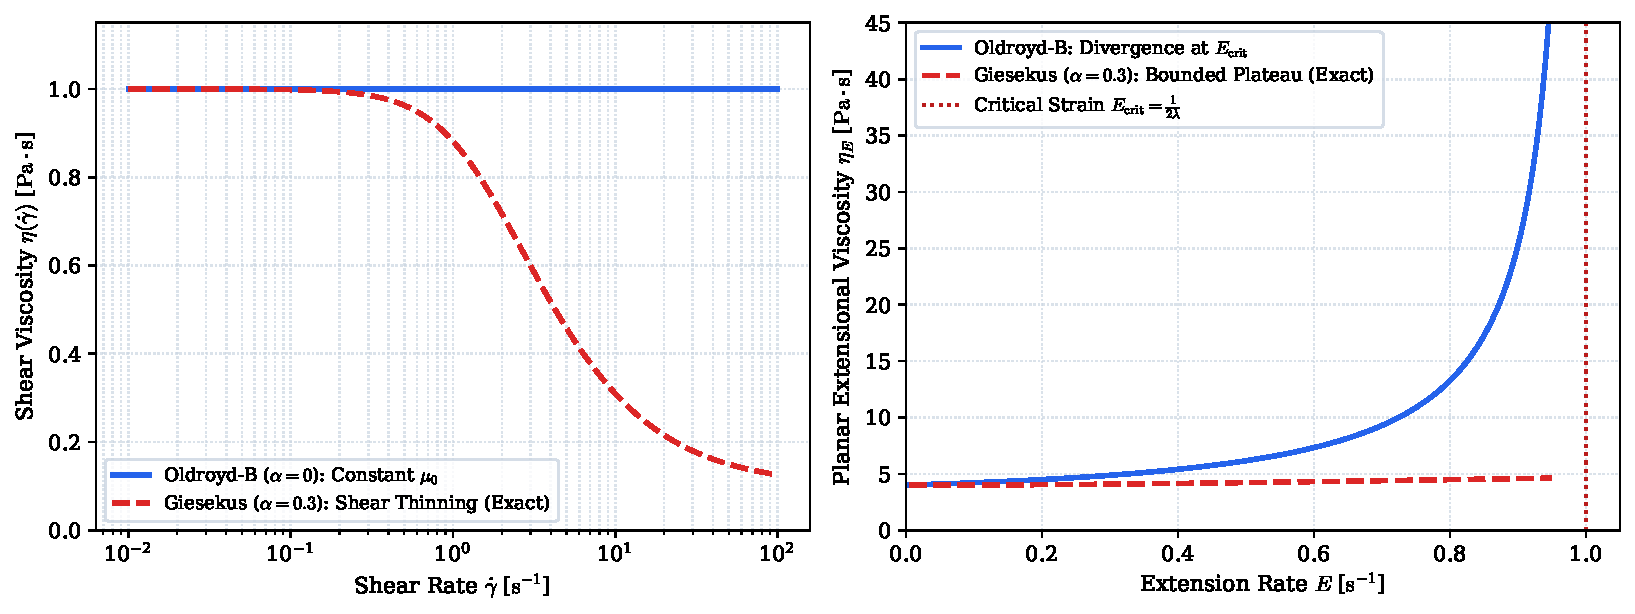
\includegraphics[width=0.92\linewidth]{media/rheological_models_concept.pdf}
    \caption{Example comparison of rheological model responses: (a) steady shear viscosity $\eta(\dot{\gamma})$ as a function of shear rate, illustrating the constant Newtonian-like plateau of Oldroyd-B ($\alpha = 0$) versus the non-linear shear-thinning response of Giesekus ($\alpha > 0$); (b) planar extensional viscosity $\eta_E(E)$ as a function of extension rate, contrasting the unphysical asymptotic divergence of Oldroyd-B at the critical strain threshold $E_{\mathrm{crit}} = 1/(2\lambda)$ with the bounded saturation plateau provided by non-linear closures.}
    \label{fig:rheological_models_concept}
\end{figure}

% ============================================================
% 2.4 NONDIMENSIONALIZATION AND GOVERNING EQUATIONS
% ============================================================
\section{Dimensionless Governing Equations}
\label{sec:nondimensionalization}

Nondimensionalization scales physical variables to order unity and establishes the
governing dimensionless groups \cite{owens2002computational}. In low-Reynolds
viscoelastic flows, scaling by a viscous stress unit rather than an inertial dynamic
pressure improves numerical conditioning and balances the magnitudes of the governing
differential operators.

\subsection{Reference Scales and Dimensionless Parameters}
\label{subsec:reference_scales}
We choose reference length $H_{\mathrm{ref}}$ (the roller radius $R$),
reference velocity $U_{\mathrm{ref}}$ (the roller surface peripheral speed $u_{\mathrm{roll}}$),
and a characteristic dynamic viscosity scale $\eta_0$ (taken as the baseline total viscosity $\mu_0$).
The dimensionless variables are defined as:
\begin{equation}
    \boldsymbol{x}^{*} = \frac{\boldsymbol{x}}{H_{\mathrm{ref}}}, \quad
    \boldsymbol{u}^{*} = \frac{\boldsymbol{u}}{U_{\mathrm{ref}}}, \quad
    p^{*} = \frac{p}{\frac{\eta_0 U_{\mathrm{ref}}}{H_{\mathrm{ref}}}}, \quad
    \boldsymbol{\tau}^{*} = \frac{\boldsymbol{\tau}}{\frac{\eta_0 U_{\mathrm{ref}}}{H_{\mathrm{ref}}}} .
    \label{eq:dimless_variables}
\end{equation}
Dropping asterisks for notational simplicity, the flow regime is governed by three fundamental dimensionless groups:
\begin{align}
    Re &= \frac{\rho U_{\mathrm{ref}} H_{\mathrm{ref}}}{\eta_0} \quad &\text{(Reynolds number)}, \label{eq:reynolds_def} \\
    Wi &= \frac{\lambda U_{\mathrm{ref}}}{H_{\mathrm{ref}}} \quad &\text{(Weissenberg number)}, \label{eq:weissenberg_def} \\
    \beta &= \frac{\mu_s}{\mu_0} = \frac{\mu_s}{\mu_s + \mu_p} \quad &\text{(Viscosity ratio)} . \label{eq:viscosity_ratio_def}
\end{align}
Each dimensionless group carries a precise physical meaning:
\begin{itemize}
    \item \textbf{Reynolds number ($Re$)}: Compares convective inertial forces to viscous dissipation forces.
    In the present benchmark, $Re \ll 1$, placing the system firmly in the laminar creeping flow (Stokes) regime.
    \item \textbf{Weissenberg number ($Wi$)}: Compares the characteristic elastic relaxation time of the polymer $\lambda$
    to the characteristic kinematic timescale of the flow $H_{\mathrm{ref}}/U_{\mathrm{ref}}$.
    It quantifies the degree of flow-induced macromolecular orientation and elastic non-linearity.
    \item \textbf{Viscosity ratio ($\beta$)}: Measures the fraction of total viscosity contributed by the Newtonian solvent.
    The limits $\beta = 1$ and $\beta \to 0$ correspond to a purely Newtonian fluid and a solvent-free polymer melt, respectively.
    The dimensionless solvent and polymeric viscosities are given by $\mu_s^* = \beta$ and $\mu_p^* = 1 - \beta$.
\end{itemize}

\subsection{Dimensionless Governing System}
\label{subsec:dimensionless_vector_system}
Expressed in terms of dimensionless variables, the steady planar governing equations become:
\begin{align}
    \nabla \cdot \boldsymbol{u} &= 0 , \label{eq:dimless_mass} \\
    Re (\boldsymbol{u} \cdot \nabla \boldsymbol{u}) + \nabla p - \beta \nabla^2 \boldsymbol{u} - \nabla \cdot \boldsymbol{\tau} &= \boldsymbol{0} , \label{eq:dimless_momentum} \\
    \boldsymbol{\mathcal{G}}(\boldsymbol{\tau}) + Wi \left( \boldsymbol{u} \cdot \nabla \boldsymbol{\tau} - (\nabla \boldsymbol{u}) \boldsymbol{\tau} - \boldsymbol{\tau} (\nabla \boldsymbol{u})^T \right) - 2(1 - \beta) \boldsymbol{D} &= \boldsymbol{0} , \label{eq:dimless_constitutive_unified}
\end{align}
where the constitutive operator $\boldsymbol{\mathcal{G}}(\boldsymbol{\tau})$ provides a unified closure for the models under investigation:
\begin{equation}
    \boldsymbol{\mathcal{G}}(\boldsymbol{\tau}) = 
    \begin{cases}
        \boldsymbol{\tau} & \text{(Oldroyd-B)}, \\[1ex]
        \boldsymbol{\tau} + \frac{\alpha Wi}{1 - \beta} \boldsymbol{\tau}^2 & \text{(Giesekus)}, \\[1ex]
        \left(1 + \frac{\varepsilon Wi}{1 - \beta} \text{tr}(\boldsymbol{\tau})\right) \boldsymbol{\tau} & \text{(Linear PTT)} .
    \end{cases}
    \label{eq:constitutive_operator_cases}
\end{equation}

% ============================================================
% 2.5 THE FOUR-ROLL MILL BENCHMARK AND BOUNDARY CONDITIONS
% ============================================================
\section{Four-Roll Mill}
\label{sec:four_roll_mill_bcs}

The four-roll mill is a classic benchmark designed to generate controlled two-dimensional planar extensional flow
with a central stagnation point \cite{taylor1934formation, fuller1980flow, fuller1981flow, bentley1986experimental}.
Originally introduced by Taylor \cite{taylor1934formation} and systematically analyzed by Fuller and Leal \cite{fuller1980flow, fuller1981flow},
it provides an ideal apparatus for investigating macromolecular deformation away from solid walls.
As illustrated conceptually in Figure~\ref{fig:4roll_concept}, the setup comprises four cylindrical rollers placed symmetrically inside a closed square cavity.

\begin{figure}[htbp]
    \centering
    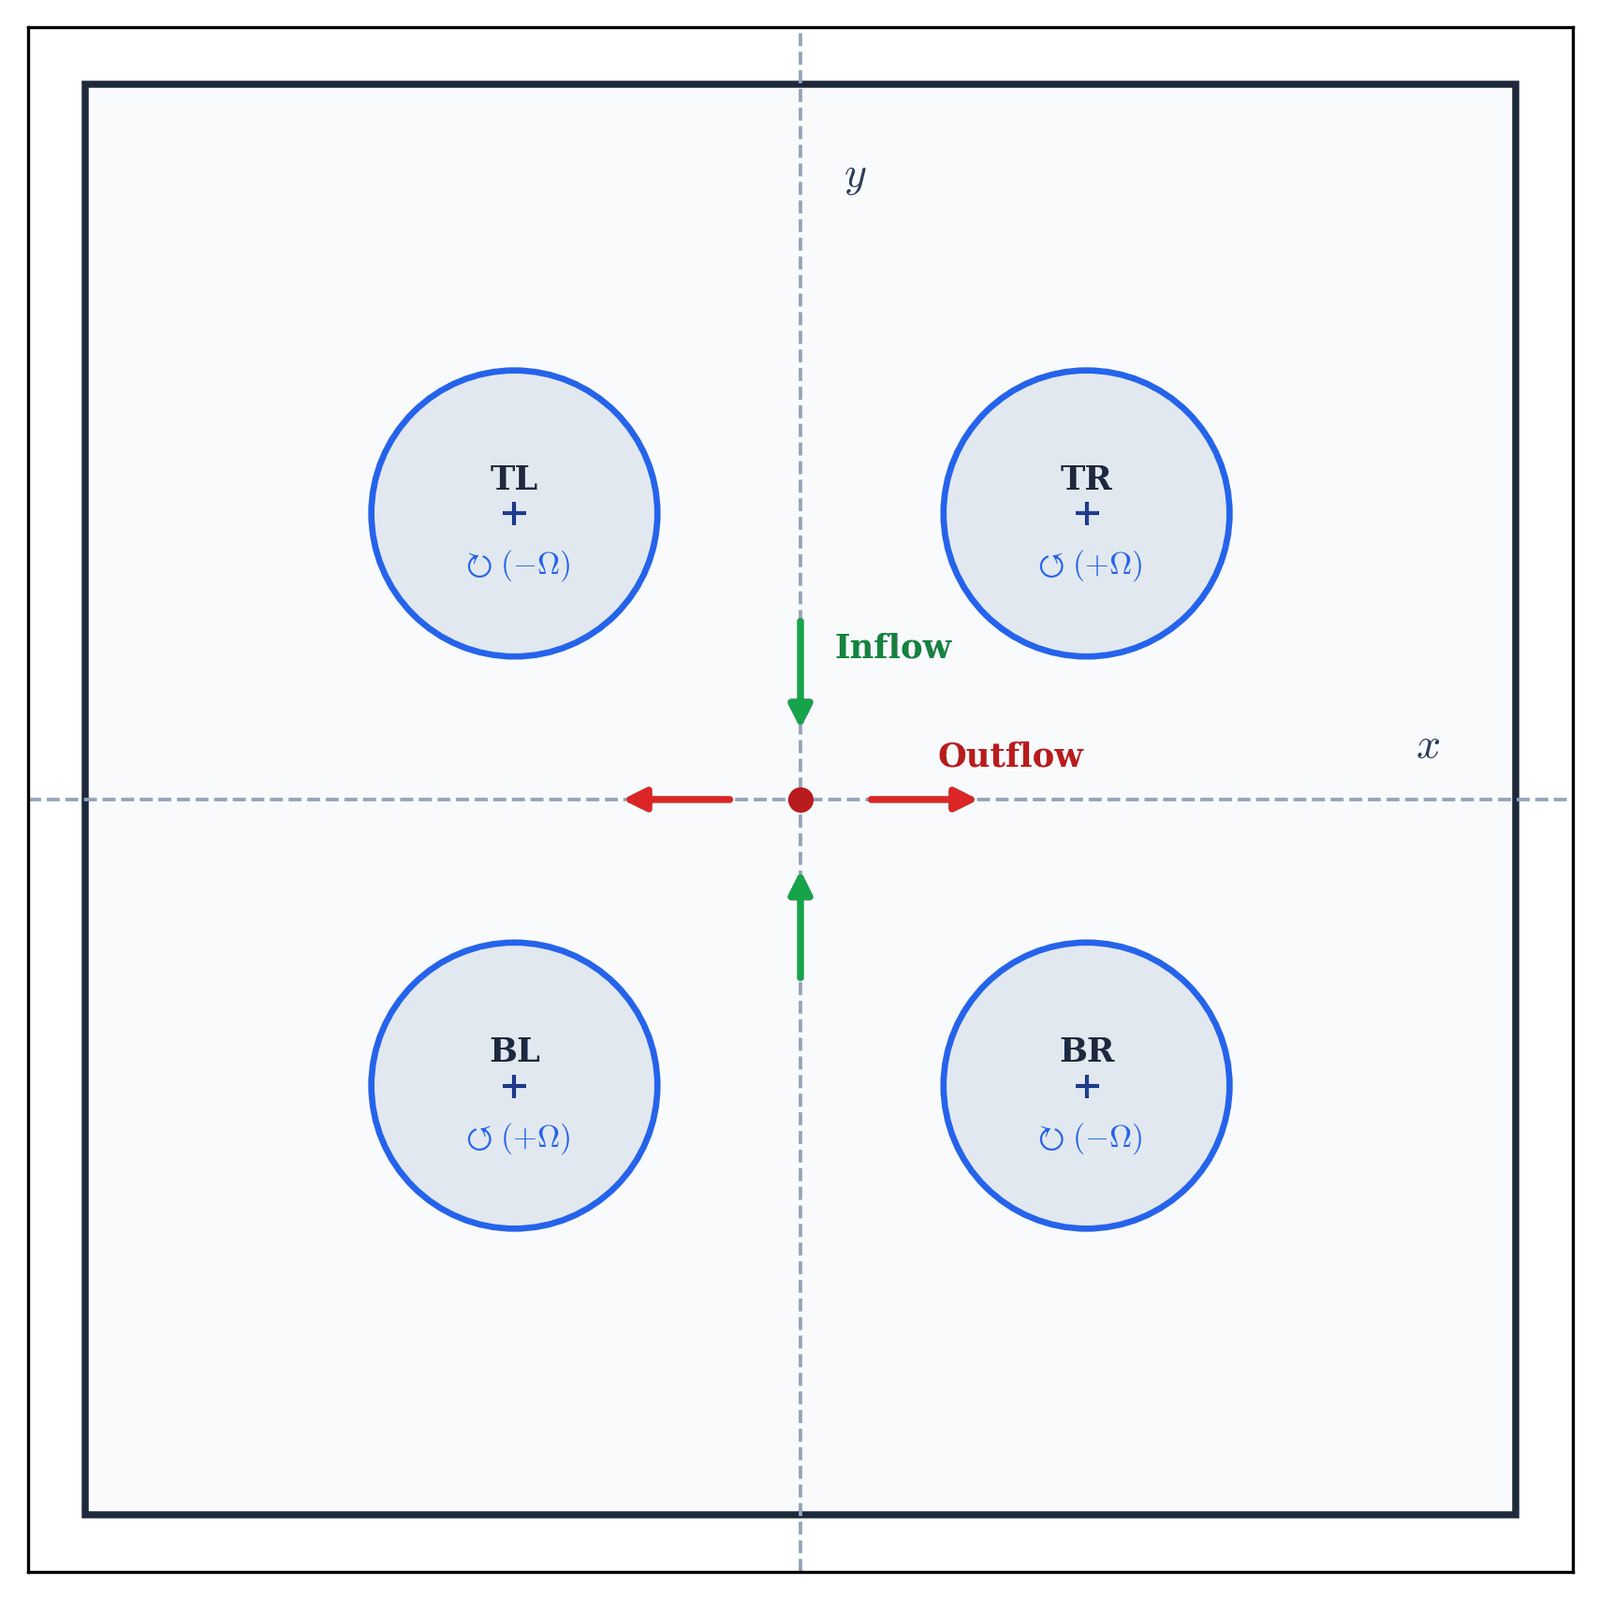
\includegraphics[width=0.58\linewidth]{media/4roll_mill_concept.png}
    \caption{Conceptual diagram of the four-roll mill geometry, illustrating the four rotating cylinders (adjacent rolls counter-rotate with angular velocity $\Omega$, diagonal rolls co-rotate), the central hyperbolic stagnation point $(0,0)$, and the resulting elongational inflow and outflow directions.}
    \label{fig:4roll_concept}
\end{figure}

\subsection{Flow Index Parameter}
\label{subsec:4roll_kinematics}
In the central region bounded by the four rollers, the velocity field can be represented
as a linear superposition of extension and solid-body rotation \cite{fuller1980flow, fuller1981flow}:
\begin{equation}
    \boldsymbol{u}(x, y) = \begin{pmatrix} E x + \omega y \\ -E y - \omega x \end{pmatrix} ,
    \label{eq:kinematic_general}
\end{equation}
where $E \ge 0$ is the extension rate and $\omega \ge 0$ is the angular rotation rate.
To quantify the relative magnitude of extension versus rotation,
we define a dimensionless flow type parameter $\chi \in [-1, 1]$:
\begin{equation}
    \chi = \frac{E - \omega}{E + \omega} .
    \label{eq:flow_parameter_chi}
\end{equation}
Depending on roller rotation speeds and directions, this local kinematics covers three canonical flow regimes
(in Figure~\ref{fig:four_roll_flow_regimes}):
\begin{itemize}
    \item $\chi = +1$ ($\omega = 0$): \textbf{Pure Planar Extensional Flow}.
    Generated when adjacent rollers counter-rotate symmetrically (diagonal rollers co-rotate).
    Fluid elements experience pure elongation along $x$ and compression along $y$, producing hyperbolic streamlines $x y = \text{const}$.
    \item $\chi = 0$ ($E = \omega$): \textbf{Simple Shear Flow}.
    Characterized by equal strain and rotation rates, producing rectilinear shear streamlines locally near the origin.
    \item $\chi = -1$ ($E = 0$): \textbf{Pure Solid-Body Rotation}.
    Generated when rollers rotate in unison to drive bulk cavity circulation, resulting in concentric circular streamlines without stretching.
\end{itemize}

\begin{figure}[htbp]
    \centering
    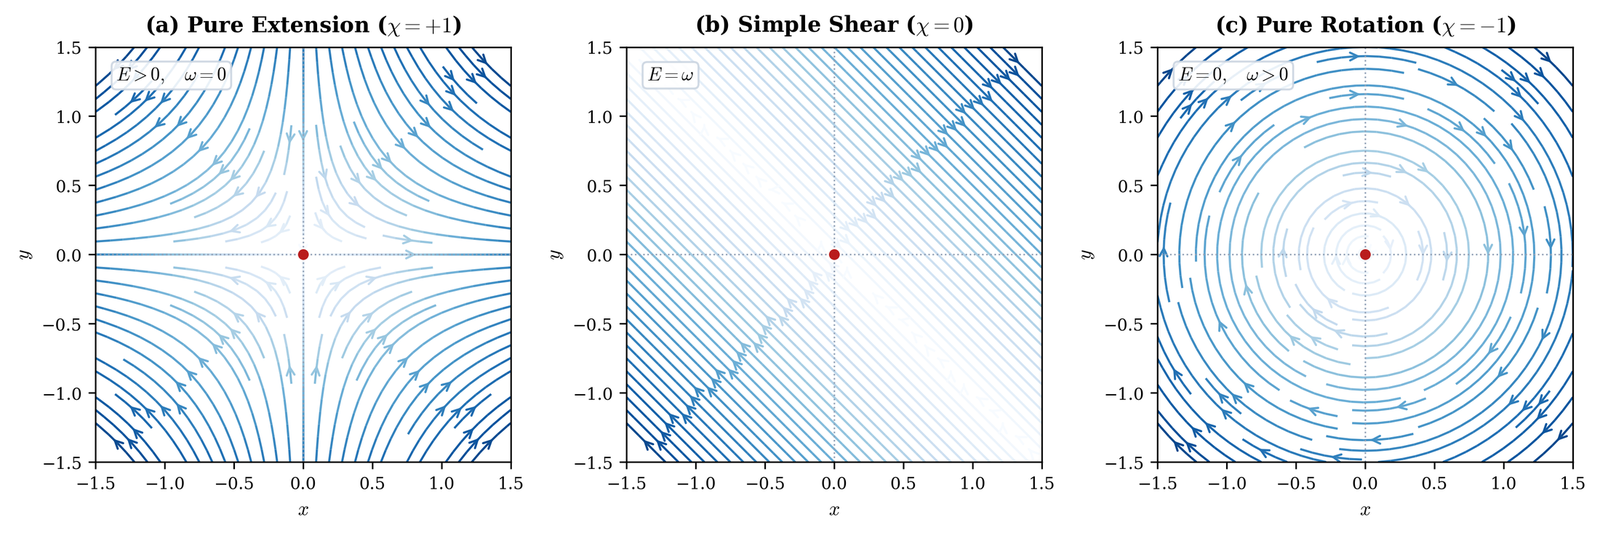
\includegraphics[width=\linewidth]{media/four_roll_flow_regimes.png}
    \caption{Streamline patterns of the two-dimensional linear flow field in
    Equation~\eqref{eq:kinematic_general} for the three canonical regimes of the flow
    classification parameter $\chi$: (a) pure planar extension ($\chi = +1$), (b)
    simple shear ($\chi = 0$), and (c) pure solid-body rotation ($\chi = -1$). The
    red marker indicates the central stagnation point $(0,0)$.}
    \label{fig:four_roll_flow_regimes}
\end{figure}

\subsection{Stagnation Point}
\label{subsec:stagnation_point}
In the planar extensional regime ($\chi = +1$), the velocity vanishes identically at the cavity center:
\begin{equation}
    \boldsymbol{u}(0, 0) = \boldsymbol{0} .
\end{equation}
Along the vertical inflow streamline ($x = 0$), incoming fluid parcels decelerate toward zero velocity,
reaching asymptotically long residence times near the origin.
This kinematics allows elastic strain to accumulate over durations comparable to or exceeding the polymer relaxation time $\lambda$,
making the four-roll mill an ideal benchmark for probing strong extensional stresses far from solid walls.

\subsection{Geometric Setup and Operating Parameters}
\label{subsec:geometry_params}
Following the established benchmark setup of D'Avino et al. \cite{davino2017numerical},
we define the physical dimensions and operating conditions of the apparatus:
\begin{itemize}
    \item \textbf{Square cavity}: Side length $L = 50\,\mathrm{mm}$ spanning the domain $[-25, 25]\,\mathrm{mm}$.
    \item \textbf{Cylindrical rollers}: Radius $R = 5\,\mathrm{mm}$ ($H_{\mathrm{ref}} = R = 0.1 L$).
    \item \textbf{Roller centers}: Located symmetrically at $(\pm 10, \pm 10)\,\mathrm{mm}$ ($d_{\mathrm{roll}} = 10\,\mathrm{mm}$).
    \item \textbf{Roller surface speed}: Peripheral velocity $u_{\mathrm{roll}} = \Omega R = 8.333 \times 10^{-3}\,\mathrm{m/s}$.
    \item \textbf{Dimensionless domain}: In units of $H_{\mathrm{ref}} = R$, the computational domain spans $[-5, 5]^2$,
    with roller centers located at $(\pm 2.0, \pm 2.0)$ and non-dimensional roller radius $R^* = 1.0$.
\end{itemize}

As shown in Figure~\ref{fig:4roll_geometry}, these dimensions define the operational space and solid boundaries of the cavity.

\begin{figure}[htbp]
    \centering
    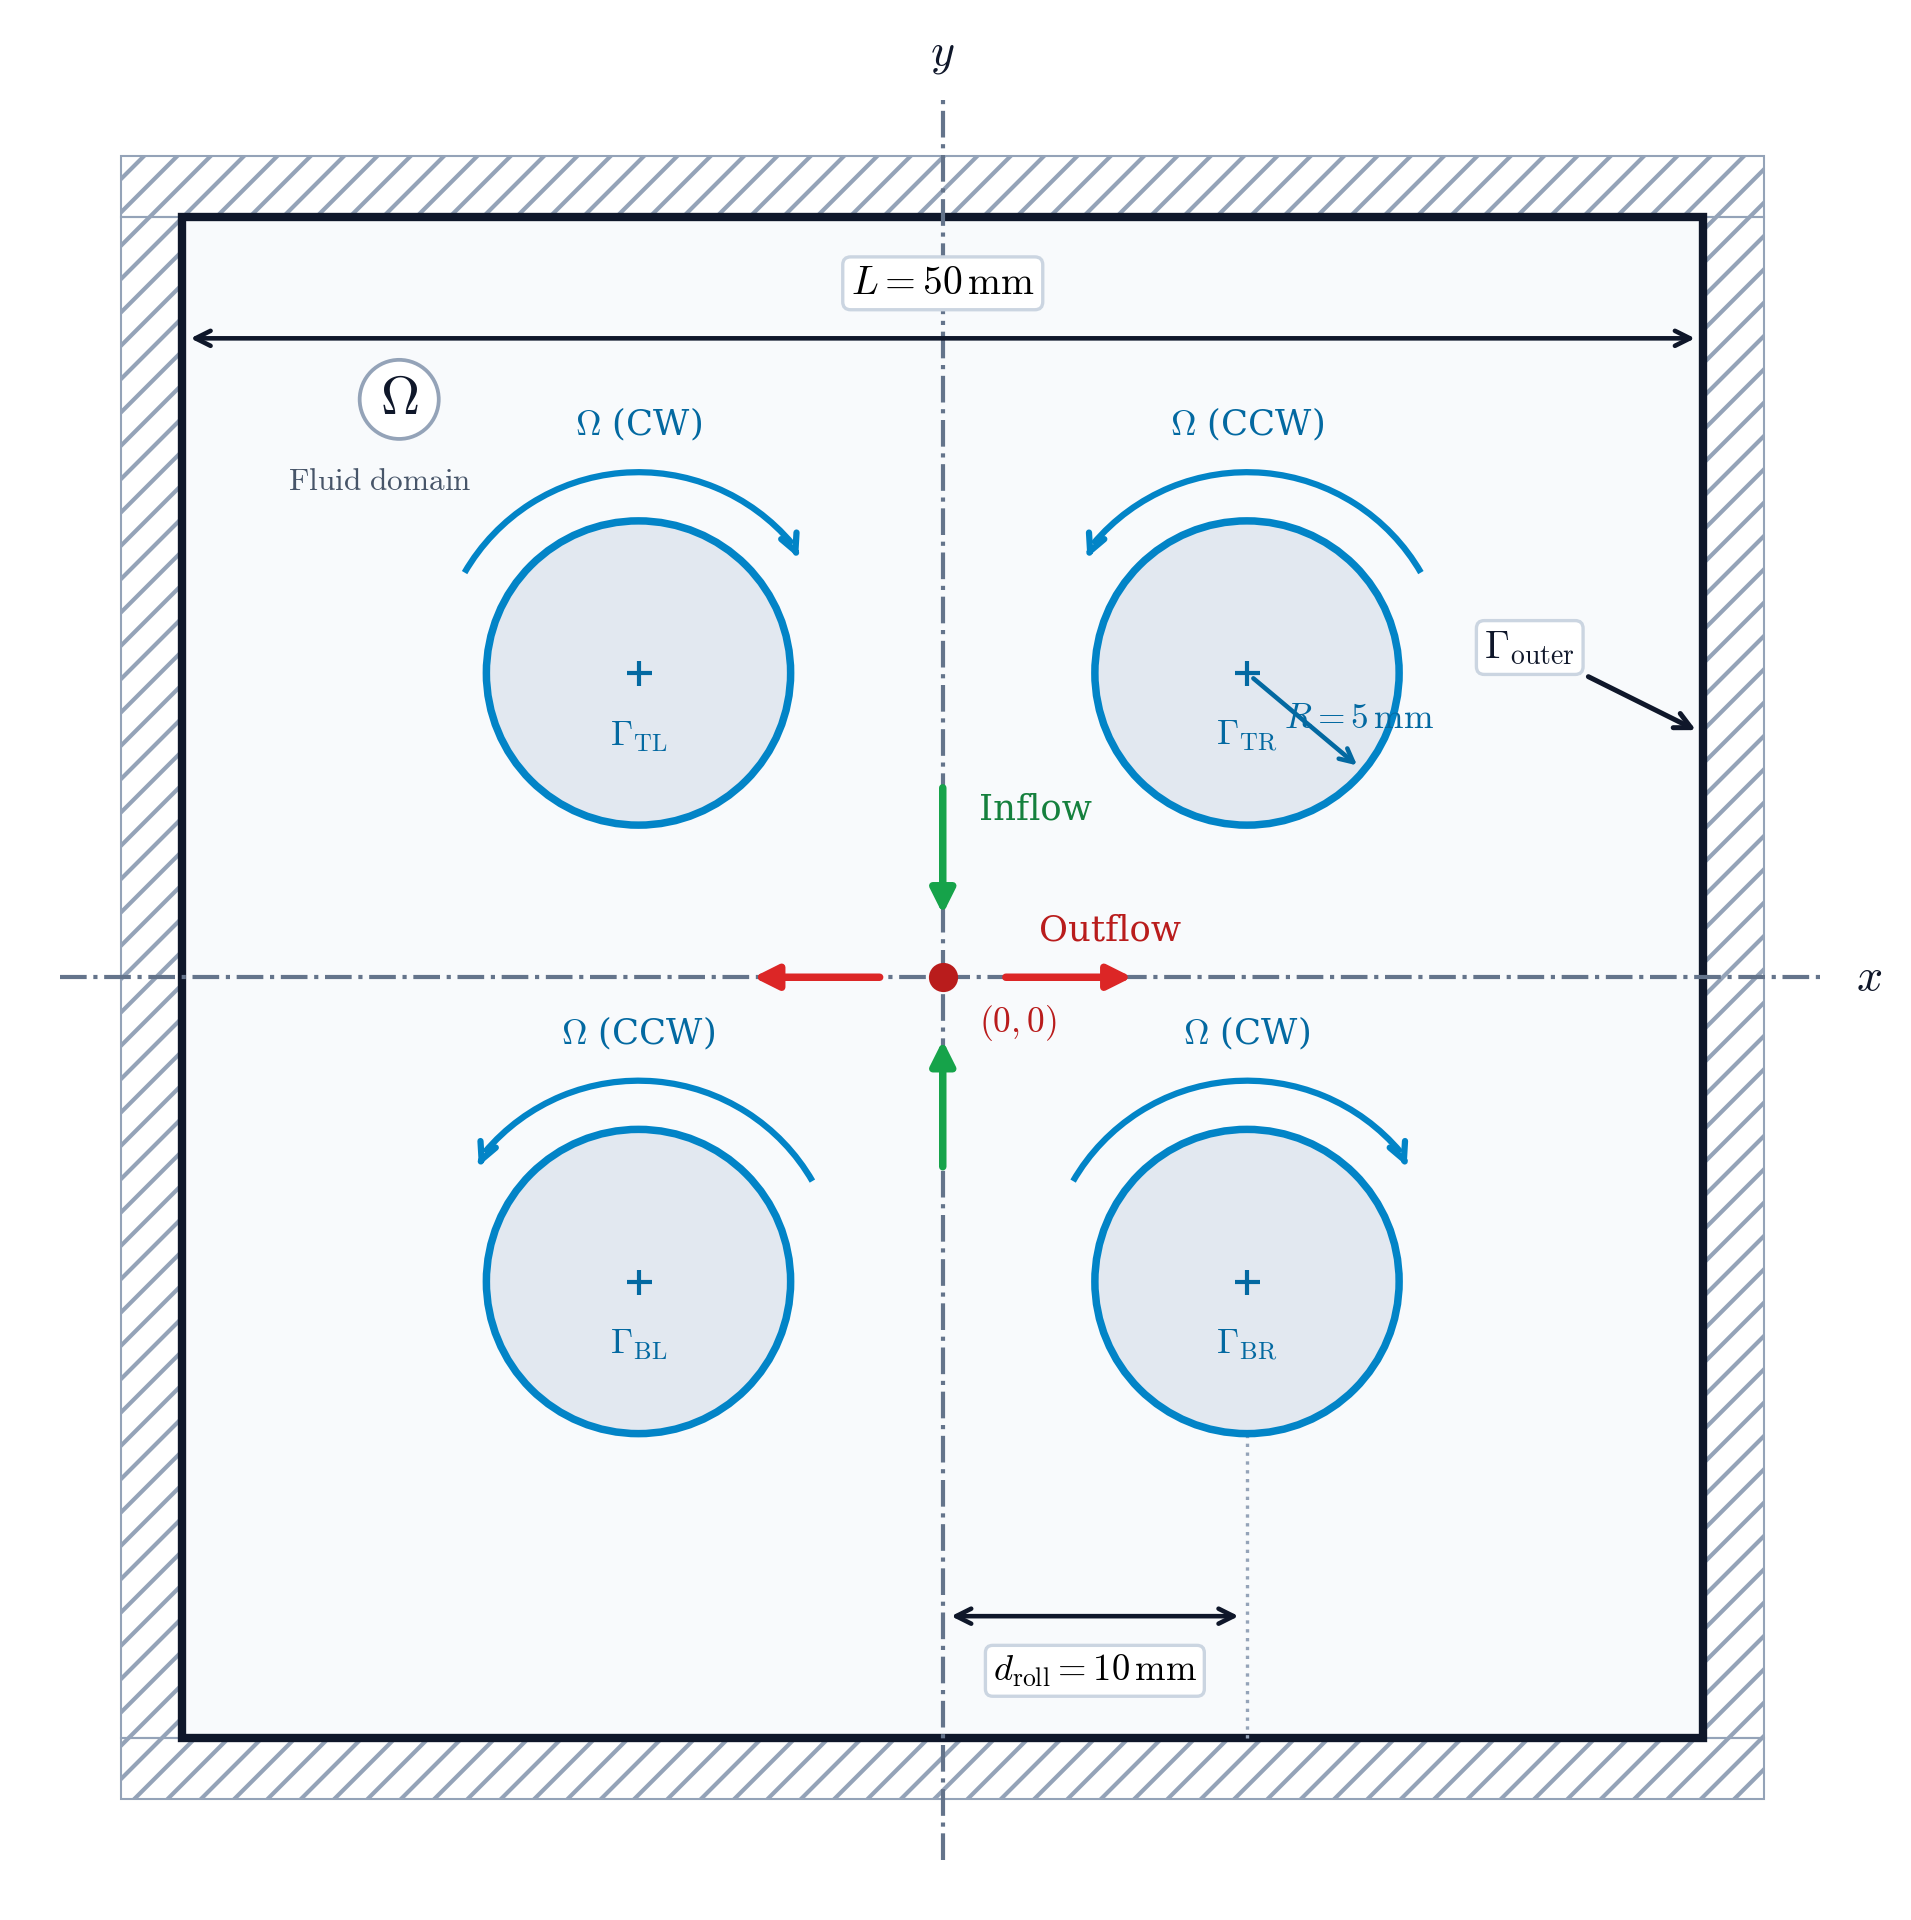
\includegraphics[width=0.68\linewidth]{media/4roll_mill_geometry_thesis.png}
    \caption{Detailed geometric dimensions and coordinate setup of the four-roll mill: square cavity side $L = 50\,\mathrm{mm}$, cylinder radii $R = 5\,\mathrm{mm}$, roller center offset $d_{\mathrm{roll}} = 10\,\mathrm{mm}$, Cartesian axes $(x, y)$, and peripheral rotation directions with angular velocity $\Omega$.}
    \label{fig:4roll_geometry}
\end{figure}

The geometric, fluid physical, and characteristic dimensionless parameters investigated in this work
are organized systematically in Table~\ref{tab:physical_parameters}.

\begin{table}[htbp]
    \centering
    \caption{Geometric, physical, and dimensionless parameters of the four-roll mill benchmark.}
    \label{tab:physical_parameters}
    \begin{tabular}{lccc}
        \hline
        \textbf{Parameter} & \textbf{Symbol} & \textbf{Value / Range} & \textbf{Unit} \\
        \hline
        \multicolumn{4}{l}{\textit{Geometric and Kinematic Setup}} \\
        Cavity side length & $L$ & $0.05$ & $\mathrm{m}$ \\
        Roller radius (reference length) & $H_{\mathrm{ref}} = R$ & $0.005$ & $\mathrm{m}$ \\
        Roller center offset & $d_{\mathrm{roll}}$ & $0.010$ & $\mathrm{m}$ \\
        Roller peripheral velocity & $u_{\mathrm{roll}} = U_{\mathrm{ref}}$ & $8.333 \times 10^{-3}$ & $\mathrm{m/s}$ \\
        \hline
        \multicolumn{4}{l}{\textit{Fluid Physical Properties}} \\
        Fluid density & $\rho$ & $1000$ & $\mathrm{kg/m^3}$ \\
        Characteristic viscosity scale & $\eta_0 = \mu_0$ & $1.0$ & $\mathrm{Pa\cdot s}$ \\
        Solvent dynamic viscosity & $\mu_s$ & $0.1\text{--}0.5$ & $\mathrm{Pa\cdot s}$ \\
        Polymer dynamic viscosity & $\mu_p$ & $0.5\text{--}0.9$ & $\mathrm{Pa\cdot s}$ \\
        Polymer relaxation time & $\lambda$ & $0.05\text{--}1.0$ & $\mathrm{s}$ \\
        \hline
        \multicolumn{4}{l}{\textit{Dimensionless Governing Groups}} \\
        Reynolds number & $Re$ & $0.0417 \ll 1$ & $-$ \\
        Weissenberg number & $Wi$ & $0.083\text{--}1.667$ & $-$ \\
        Viscosity ratio & $\beta$ & $0.1\text{--}0.5$ & $-$ \\
        \hline
    \end{tabular}
\end{table}

\subsection{Boundary Conditions}
\label{subsec:boundary_conditions}
To complete the mathematical formulation, boundary conditions are imposed along allrelevant domain boundaries:
\begin{enumerate}
    \item \textbf{No-Slip on Roller Surfaces ($\Gamma_{\mathrm{rolls}}$)}:
    On the boundary of each cylinder $k \in \{\mathrm{TL}, \mathrm{TR}, \mathrm{BL}, \mathrm{BR}\}$,
    the fluid velocity satisfies the no-slip Dirichlet condition with specified angular rotation:
    \begin{equation}
        \boldsymbol{u}|_{\Gamma_k} = \boldsymbol{\Omega}_k \times (\boldsymbol{x} - \boldsymbol{x}_k) ,
        \label{eq:bc_velocity_rolls}
    \end{equation}
    where $\boldsymbol{x}_k$ is the roller center and the angular velocity vector is directed along the out-of-plane axis, $\boldsymbol{\Omega}_k = (0, 0, \Omega_k)^T$.
    In the planar extensional regime ($\chi = +1$),
    top-left (TL) and bottom-right (BR) cylinders rotate clockwise ($\Omega_k = -\Omega$),
    while top-right (TR) and bottom-left (BL) cylinders rotate counter-clockwise ($\Omega_k = +\Omega$),
    with peripheral angular speed $\Omega = u_{\mathrm{roll}} / R$.

    \item \textbf{No-Slip on Walls ($\Gamma_{\mathrm{outer}}$)}:
    Along the stationary external boundaries of the square cavity, the velocity vanishes identically:
    \begin{equation}
        \boldsymbol{u}|_{\Gamma_{\mathrm{outer}}} = \boldsymbol{0} .
        \label{eq:bc_outer_walls}
    \end{equation}

    \item \textbf{Pressure Gauge Fixing}:
    Because pressure appears in the momentum balance~\eqref{eq:dimless_momentum} exclusively through its spatial gradient $\nabla p$,
    the pressure field is determined only up to an arbitrary additive constant ($p \to p + C$) under pure velocity Dirichlet conditions.
    To eliminate this degree of freedom, pressure is anchored with a single reference point:
    \begin{equation}
        p(\boldsymbol{x}_0) = 0 .
        \label{eq:pressure_point}
    \end{equation}
\end{enumerate}

    % !TEX root = ../main.tex
\chapter{Physics-Informed Neural Networks in Complex Rheology}
\label{chap:pinn_literature}

Feedforward deep neural networks, commonly known as Multi-Layer Perceptrons (MLPs),
provide flexible continuous approximations for non-linear functions \cite{goodfellow2016deep}.
An MLP is formed by composing a sequence of parametric functions, called \textit{layers}.
Each layer maps its inputs through a linear transformation followed by a non-linear operation.
With these layers in series, the network can represent continuous functional mappings
of arbitrary complexity without requiring explicit basis functions.

In scientific computing, neural networks represent physical fields directly as
continuous functions over spatial coordinates, rather than storing discrete state variables on a mesh.
However, using purely data-driven networks for fluid mechanics presents clear limits:
they require large amounts of labeled data, can violate conservation laws,
and cannot infer latent material properties on their own.

Physics-Informed Neural Networks (PINNs) address these limits
by embedding governing partial differential equations directly into the training loss.
The differential system formulated in Chapter~\ref{chap:fluidodynamic_background}, governed by mass conservation,
viscoelastic momentum balance, and frame-indifferent constitutive transport,
represents a coupled set of non-linear equations that poses well-known challenges to traditional mesh-based methods.
In this chapter, we formulate this continuous boundary-value problem within a Scientific Machine Learning (SciML) framework.
By embedding momentum and constitutive balances into the optimization objective through automatic differentiation,
the PINN framework enables both direct state reconstruction and inverse rheological parameter discovery without spatial discretization meshes.

% ============================================================
% 3.1 FUNDAMENTALS OF DEEP LEARNING
% ============================================================
\section{Fundamentals of Deep Learning}
\label{sec:dl_fundamentals}

Deep learning models approximate continuous mathematical functions
by learning parameters directly from data \cite{goodfellow2016deep}.
In this section, we review the fundamental building blocks of feedforward networks:
the artificial neuron, activation functions, multi-layer architectures,
loss functions, optimization algorithms, and gradient computation.

\subsection{The Artificial Neuron and Non-Linear Activation Functions}
\label{subsec:perceptron_activations}

The elementary computational unit of a neural network is the artificial neuron.
Given an input vector $\boldsymbol{x}$,
a neuron computes a linear combination of the inputs followed by a non-linear activation:
\begin{equation}
    z = \boldsymbol{w} \cdot \boldsymbol{x} + b , \qquad a = \sigma(z) ,
    \label{eq:single_neuron}
\end{equation}
where $\boldsymbol{w}$ is the weight vector, $b$ is a scalar bias, $\sigma(\cdot)$ is the activation function and $a$ is the output.
Non-linear activations are essential:
without them, composing multiple linear layers simply collapses into a single linear transformation.

In classical machine learning, piecewise-linear functions such as the Rectified Linear Unit,
$\text{ReLU}(z) = \max(0, z)$, are widely favored for their computational efficiency.
However, in scientific computing and fluid mechanics,
the network outputs parameterize continuous physical fields governed by differential equations.
These governing balance laws involve spatial derivatives of first, second, or third order,
such as viscous diffusion $\mu_s \nabla^2 \boldsymbol{u}$ or stress divergence $\nabla \cdot \boldsymbol{\tau}$.

Because the first derivative of ReLU is discontinuous and its second derivative is zero almost everywhere,
evaluating a ReLU network inside differential residuals eliminates diffusive and curvature terms.
Physics-informed models therefore require smooth, differentiable activation functions ($\mathcal{C}^2$ or higher).
In this work, we employ the Sigmoid Linear Unit (SiLU, also known as Swish) \cite{goodfellow2016deep}:
\begin{equation}
    \text{SiLU}(z) = \frac{z}{1 + e^{-z}} .
    \label{eq:silu_activation}
\end{equation}
The SiLU activation is smooth and non-monotonic.
Unlike the hyperbolic tangent ($\tanh$), which saturates toward constant values for large positive inputs,
SiLU remains active in the positive regime.
This property maintains healthy gradient propagation in flow regions with intense shear
and steep localized stress gradients, which are characteristic of viscoelastic flows.

\subsection{Multi-Layer Perceptron Architecture}
\label{subsec:mlp_architecture}

By arranging artificial neurons into sequential layers, we construct a Multi-Layer Perceptron (MLP).
The network maps an input vector $\boldsymbol{x}$ to an output prediction $\hat{\boldsymbol{u}}$
by propagating information through $L$ successive layers \cite{goodfellow2016deep}:
\begin{align}
    \boldsymbol{h}^{(1)} &= \sigma\left( \boldsymbol{W}^{(1)} \boldsymbol{x} + \boldsymbol{b}^{(1)} \right) , \nonumber \\
    \boldsymbol{h}^{(l)} &= \sigma\left( \boldsymbol{W}^{(l)} \boldsymbol{h}^{(l-1)} + \boldsymbol{b}^{(l)} \right) , \quad \text{for } l = 2, \dots, L-1 , \label{eq:mlp_layers} \\
    \hat{\boldsymbol{u}} &= \boldsymbol{W}^{(L)} \boldsymbol{h}^{(L-1)} + \boldsymbol{b}^{(L)} , \nonumber
\end{align}
where $\boldsymbol{h}^{(l)}$ denotes the hidden feature vector at layer $l$,
and $\boldsymbol{W}^{(l)}$ and $\boldsymbol{b}^{(l)}$ represent the weight matrix and bias vector of that layer.
In our implementation, the inputs $\boldsymbol{x} = (x, y)$ are spatial coordinates within the fluid cavity,
while the outputs $\hat{\boldsymbol{u}}$ parameterize the physical state variables:
the stream function $\psi$, hydrodynamic pressure $p$, and extra-stress tensor components $\boldsymbol{\tau}$.

\begin{figure}[H]
    \centering
    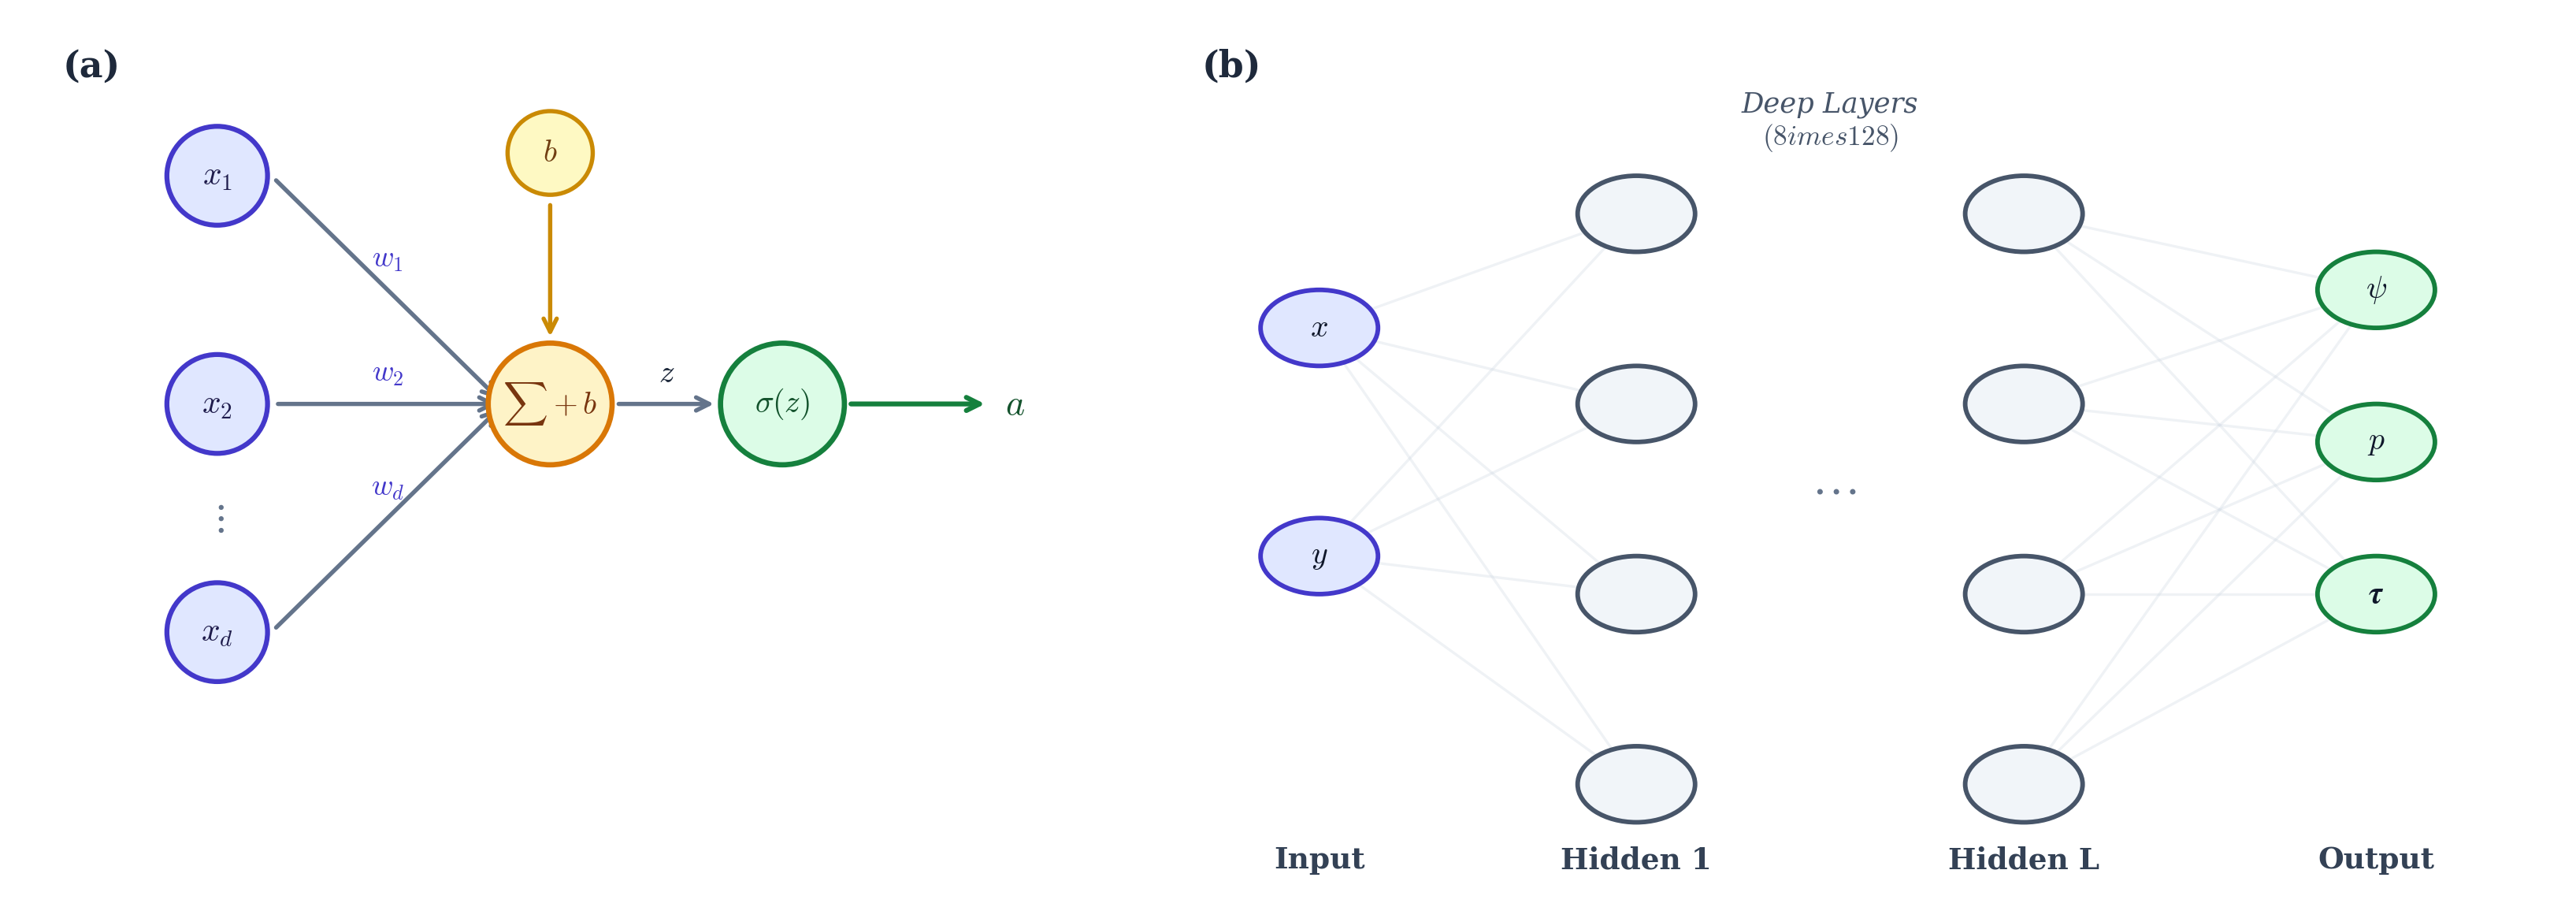
\includegraphics[width=0.82\linewidth]{media/deep_learning_mlp_diagram.png}
    \caption{Neural network representations: (a) schematic of an artificial neuron computing an affine combination $z = \boldsymbol{w} \cdot \boldsymbol{x} + b$ followed by a smooth activation $\sigma(z)$; (b) deep Multi-Layer Perceptron (MLP) architecture propagating coordinate inputs $(x, y)$ through $L$ hidden layers to parameterize continuous physical fields $(\psi, p, \boldsymbol{\tau})$.}
    \label{fig:deep_learning_mlp_diagram}
\end{figure}

A central theoretical property of MLPs is universal function approximation
\cite{cybenko1989approximation, hornik1989multilayer}:
a feedforward network with sufficient width and smooth non-linear activations
can approximate any continuous function on a compact domain to arbitrary precision.
However, universal approximation guarantees only the existence of a suitable set of weights,
not that standard gradient-based optimization will automatically find them
or that spatial derivatives will match the physical solution with equal fidelity.

\subsubsection{Importance of Weight Initialization}
\label{subsubsec:weight_initialization}

The initialization of network parameters strongly conditions the resulting optimization dynamics.
Because deep architectures compose multiple transformations and non-linearities, inappropriate initial weight magnitudes can cause layer activations and backpropagated gradients to either vanish or explode across depth \cite{goodfellow2016deep}.
In scientific computing and differential problems, where non-linear convective terms and tensor couplings are evaluated, uncalibrated initial weights can trigger extreme initial residual spikes that immediately destabilize gradient descent.
Appropriate variance-preserving initialization schemes, such as scaling parameter distributions inversely with layer widths, help preserve stable gradient flow and avoid optimization divergence.
Specific configuration choices regarding hidden and output layer initialization adopted in this work are detailed in Chapter~\ref{chap:results_discussion}.

\subsection{Loss Functions and Optimization Algorithms}
\label{subsec:optimization_solvers}

Training an MLP consists of identifying a parameter set $\boldsymbol{\theta} = \{ \boldsymbol{W}^{(l)}, \boldsymbol{b}^{(l)} \}$ that minimizes a scalar objective function $\mathcal{L}(\boldsymbol{\theta})$.
In supervised regression, the discrepancy between model predictions and target reference measurements is commonly quantified through the Mean Squared Error (MSE):
\begin{equation}
    \mathcal{L}_{\mathrm{MSE}}(\boldsymbol{\theta}) = \frac{1}{N} \sum_{i=1}^N \left\| \hat{\boldsymbol{u}}(\boldsymbol{x}_i; \boldsymbol{\theta}) - \boldsymbol{u}_i^{\mathrm{target}} \right\|_2^2 .
    \label{eq:mse_loss}
\end{equation}
Parameters are iteratively updated along descent directions derived from the loss gradient:
\begin{equation}
    \boldsymbol{\theta} \leftarrow \boldsymbol{\theta} - \eta \boldsymbol{d}_k ,
    \label{eq:gradient_descent_update}
\end{equation}
where $\eta > 0$ represents the learning rate (step size) and $\boldsymbol{d}_k$ denotes the search direction at iteration $k$.

In scientific machine learning, gradient-based solvers must navigate non-convex
loss surfaces characterized by ill-conditioned curvature and local minima.
Two widely adopted algorithms in this setting are:

\subsubsection{Adam: First Order Estimation}
\label{subsubsec:adam_optimizer}

The Adam optimizer~\cite{kingma2014adam} computes individual adaptive learning
rates for each network parameter by tracking running estimates of the first
and second moments of the loss gradient.
At iteration $k$, given the gradient $\boldsymbol{g}_k = \nabla_{\boldsymbol{\theta}} \mathcal{L}(\boldsymbol{\theta}_k)$,
the algorithm updates two vectors recursively:
\begin{align}
    \boldsymbol{m}_k &= \beta_1 \boldsymbol{m}_{k-1} + (1 - \beta_1) \boldsymbol{g}_k , \label{eq:adam_first_moment} \\
    \boldsymbol{v}_k &= \beta_2 \boldsymbol{v}_{k-1} + (1 - \beta_2) \boldsymbol{g}_k^2 , \label{eq:adam_second_moment}
\end{align}
where the square $\boldsymbol{g}_k^2$ is evaluated component-wise, and $\beta_1, \beta_2 \in [0, 1)$
are exponential decay factors (canonically set to $\beta_1 = 0.9$ and $\beta_2 = 0.999$).

These two vectors have distinct physical and optimization roles:
\begin{itemize}
    \item \textbf{First moment vector $\boldsymbol{m}_k$ (Directional Momentum)}:
        maintains an exponentially decaying average of past gradients.
        It acts as a directional inertia, accelerating descent along persistent slopes
        while dampening high-frequency oscillations across walls.
    \item \textbf{Second uncentered moment vector $\boldsymbol{v}_k$ (Adaptive Scaling)}:
        tracks the running magnitude of squared gradient components.
        By dividing the update step by $\sqrt{\boldsymbol{v}_k}$, Adam rescales the effective
        learning rate coordinate by coordinate, taking cautious smaller steps along steep,
        noisy directions and bolder steps along flat plateaus.
\end{itemize}

Because both moment vectors are initialized to zero ($\boldsymbol{m}_0 = \boldsymbol{v}_0 = \boldsymbol{0}$),
they initially exhibit a numerical bias toward zero.
Kingma and Ba~\cite{kingma2014adam} rescale $\boldsymbol{m}_k$ and $\boldsymbol{v}_k$ by $(1 - \beta_1^k)$
and $(1 - \beta_2^k)$ to correct this initial bias before updating the parameter vector $\boldsymbol{\theta}_{k+1}$.
This adaptive mechanism makes Adam particularly robust on rugged, multi-objective loss landscapes
characterized by disparate gradient scales, serving as an effective global explorer in early training.

\subsubsection{L-BFGS: Second-Order Refinement}
\label{subsubsec:lbfgs_optimizer}

While first-order methods explore the loss landscape robustly, refining physical
solutions and satisfying stiff differential equations requires incorporating
second-order curvature information.
Classical Newton methods require forming and inverting the full Hessian matrix
$\nabla_{\boldsymbol{\theta}}^2 \mathcal{L}$, which is computationally prohibitive
for neural networks containing $N \sim 10^5\text{--}10^6$ parameters ($\mathcal{O}(N^2)$
memory and $\mathcal{O}(N^3)$ inversion cost).

Quasi-Newton methods overcome this limitation by iteratively approximating the inverse
Hessian matrix $\boldsymbol{H}_k \approx (\nabla_{\boldsymbol{\theta}}^2 \mathcal{L})^{-1}$
using only successive parameter displacements $\boldsymbol{s}_k = \boldsymbol{\theta}_{k+1} - \boldsymbol{\theta}_k$
and gradient variations $\boldsymbol{y}_k = \nabla_{\boldsymbol{\theta}} \mathcal{L}_{k+1} - \nabla_{\boldsymbol{\theta}} \mathcal{L}_k$.
The classic BFGS update formula is given by~\cite{nocedal1980updating}:
\begin{equation}
    \boldsymbol{H}_{k+1} = (\boldsymbol{I} - \rho_k \boldsymbol{s}_k \boldsymbol{y}_k^\top) \boldsymbol{H}_k (\boldsymbol{I} - \rho_k \boldsymbol{y}_k \boldsymbol{s}_k^\top) + \rho_k \boldsymbol{s}_k \boldsymbol{s}_k^\top , \qquad \rho_k = \frac{1}{\boldsymbol{y}_k^\top \boldsymbol{s}_k} .
    \label{eq:bfgs_inverse_hessian_update}
\end{equation}

To avoid storing the dense $N \times N$ matrix $\boldsymbol{H}_{k+1}$, the
Limited-memory BFGS (L-BFGS) algorithm~\cite{nocedal1980updating, liu1989limited}
stores only the $m$ most recent vector pairs $\{ \boldsymbol{s}_i, \boldsymbol{y}_i \}_{i=k-m}^{k-1}$
(typically $m \in [10, 50]$).
The descent direction is then evaluated on the fly via an efficient two-loop recursion
algorithm, dramatically reducing the memory footprint from $\mathcal{O}(N^2)$ to $\mathcal{O}(m N)$.
The step length along this direction is calibrated through a line search ensuring
sufficient decrease of the objective function.
When evaluated over full collocation batches in double precision (FP64), L-BFGS exhibits
fast superlinear asymptotic convergence, making it ideal for the final refinement stage
of PINN solvers.


\subsection{Backpropagation}
\label{subsec:backpropagation}

To update network parameters via gradient descent,
we compute the partial derivatives of the scalar loss with respect to all weights and biases, $\nabla_{\boldsymbol{\theta}} \mathcal{L}$.
Evaluating these gradients through individual numerical perturbations would be computationally prohibitive.

Instead, neural networks compute analytical gradients using the \textit{Automatic Differentiation (AD)} algorithm \cite{baydin2018automatic}.
Automatic differentiation evaluates derivatives to machine precision by applying the chain rule to elementary operations along the computational graph.
In standard machine learning, reverse-mode AD is widely known as the \textit{backpropagation} algorithm, primarily employed to evaluate the gradient of the scalar loss with respect to network parameters.

This reverse-mode automatic differentiation evaluates all parameter gradients simultaneously
at a computational cost comparable to a single forward pass,
making deep network training feasible.

% ============================================================
% 3.2 WHY NEURAL NETWORKS? CAPABILITIES AND PHYSICAL LIMITS
% ============================================================
\section{Neural Networks: Capabilities and Physical Limitations}
\label{sec:why_neural_networks}

\subsection{Key Advantages}
\label{subsec:capabilities_universal}

Neural networks offer distinctive characteristics that make them attractive for continuous physical modeling:
\begin{enumerate}
    \item \textbf{High-Dimensional Functional Approximation}: The universal approximation capacity 
    allows neural networks to represent complex, coupled physical fields (velocities, pressures, and stress tensors) 
    within a unified functional representation, without requiring specialized interpolation elements for each variable.

    \item \textbf{Meshless Representation}: Traditional grid-based methods 
    (Finite Element, Finite Volume, and Finite Difference Methods) represent state variables 
    exclusively at discrete vertices or cell centers, relying on explicit mesh connectivity. 
    In contrast, a neural network provides a continuous, globally defined mapping $\boldsymbol{x} \mapsto \hat{\boldsymbol{u}}(\boldsymbol{x})$ 
    over the entire domain, capable of being evaluated at arbitrary spatial coordinates. 
    However, being meshless does not imply freedom from geometric considerations: defining the domain, 
    enforcing boundary conditions, and designing effective collocation point distributions remain essential 
    and influential steps.
    \item \textbf{Hardware Acceleration and Differentiability}: Modern deep learning frameworks 
    are built upon dense linear algebra operations optimized for parallel accelerator hardware (GPUs and TPUs), 
    and provide built-in automatic differentiation for computing spatial derivatives of the represented fields.
\end{enumerate}

\subsection{Limits of Purely Data-Driven Machine Learning}
\label{subsec:black_box_limits}

Despite their high expressivity, deploying purely data-driven black-box networks
to fluid mechanics and non-Newtonian rheology reveals fundamental limitations:
\begin{itemize}
    \item \textbf{Data scarcity in experimental rheology}:
    Deep neural networks typically rely on large labeled datasets.
    In fluid experiments, acquiring dense velocity fields via Particle Image Velocimetry (PIV) is labor-intensive,
    while non-intrusive measurements of internal extra-stress components are very hard to obtain in complex geometries.
    \item \textbf{Absence of physical grounding}:
    Purely data-driven models minimize empirical loss on discrete observations without physical constraints.
    Consequently, their predictions often violate incompressibility ($\nabla \cdot \boldsymbol{u} \neq 0$),
    momentum balance, and constitutive laws, generating non-physical artifacts when interpolating or extrapolating.
    \item \textbf{Overfitting}:
    In sparse-data regimes, over-parameterized networks can easily fit measurement noise,
    obtaining low training errors while losing accuracy in unmonitored regions.
    \item \textbf{Inability to discover governing parameters}:
    Black-box models learn input-output mappings,
    but cannot extract underlying physical properties, such as relaxation times or polymeric viscosities, that govern flow dynamics.
\end{itemize}

These limitations show that data alone are insufficient for scientific modeling in rheology,
motivating frameworks that embed physical conservation laws directly into the loss function.

% ============================================================
% 3.3 THE PINN PARADIGM: TRAINING, MESHLESS NATURE, AND NO OVERFITTING
% ============================================================
\section{Physics-Informed Neural Network}
\label{sec:pinn_paradigm}

The Physics-Informed Neural Network (PINN) framework, formalized by Raissi, Perdikaris, and Karniadakis \cite{raissi2019physics},
addresses the problems of purely data-driven modeling
by incorporating differential partial equations directly into the network training objective.

\subsection{Physics-Constrained Loss Formulation}
\label{subsec:pinn_loss_formulation}

Following the unified boundary-value problem (BVP) notation established in the scientific machine learning literature \cite{cuomo2022scientific}, consider a physical state described by a vector of continuous fields $\boldsymbol{u}(\boldsymbol{x})$ defined over a spatial domain $\Omega \subset \mathbb{R}^d$ bounded by $\partial \Omega$:
\begin{align}
    \mathcal{F}[\boldsymbol{u}(\boldsymbol{x}); \boldsymbol{\lambda}] &= \boldsymbol{0} , \quad \boldsymbol{x} \in \Omega , \label{eq:general_pde_operator} \\
    \mathcal{B}[\boldsymbol{u}(\boldsymbol{x})] &= \boldsymbol{g}(\boldsymbol{x}) , \quad \boldsymbol{x} \in \partial \Omega , \label{eq:general_bc_operator}
\end{align}
where:
\begin{itemize}
    \item $\boldsymbol{u}(\boldsymbol{x})$ denotes the physical state variables (in our viscoelastic framework, $\boldsymbol{u} = (\psi, p, \boldsymbol{\tau})$, comprising stream function, pressure, and extra-stress tensor components);
    \item $\mathcal{F}$ is a general non-linear differential operator encoding the governing field equations (mass conservation, momentum balance, and constitutive transport equations);
    \item $\boldsymbol{\lambda}$ denotes physical or constitutive parameters governing the flow dynamics (such as solvent viscosity, polymeric viscosity, and relaxation time);
    \item $\mathcal{B}$ denotes the boundary operator enforcing kinematic constraints on the boundaries $\partial \Omega$ (such as no-slip conditions along solid walls and prescribed angular velocities on roller surfaces), with prescribed boundary values $\boldsymbol{g}(\boldsymbol{x})$.
\end{itemize}

In a PINN, the continuous solution fields are parameterized by a deep neural network surrogate $\hat{\boldsymbol{u}}(\boldsymbol{x}; \boldsymbol{\theta})$ parameterized by weights and biases $\boldsymbol{\theta}$. Evaluating the governing differential operator on the network outputs via automatic differentiation defines the pointwise differential residual:
\begin{equation}
    \boldsymbol{f}(\boldsymbol{x}; \boldsymbol{\theta}, \boldsymbol{\lambda}) \equiv \mathcal{F}[\hat{\boldsymbol{u}}(\boldsymbol{x}; \boldsymbol{\theta}); \boldsymbol{\lambda}] .
    \label{eq:pde_residual_def}
\end{equation}
The network parameters $\boldsymbol{\theta}$, alongside any unknown physical parameters $\boldsymbol{\lambda}$ in inverse problems, are optimized simultaneously by minimizing a composite multi-objective loss:
\begin{equation}
    \mathcal{L}_{\mathrm{total}}(\boldsymbol{\theta}, \boldsymbol{\lambda}) = w_{\mathrm{data}} \mathcal{L}_{\mathrm{data}} + w_{\mathrm{bc}} \mathcal{L}_{\mathrm{bc}} + w_{\mathrm{pde}} \mathcal{L}_{\mathrm{pde}} ,
    \label{eq:composite_loss_pinn}
\end{equation}
where each individual loss component is evaluated as:
\begin{align}
    \mathcal{L}_{\mathrm{data}} &= \frac{1}{N_{\mathrm{data}}} \sum_{i=1}^{N_{\mathrm{data}}} \left\| \hat{\boldsymbol{u}}(\boldsymbol{x}_i^{\mathrm{data}}) - \boldsymbol{u}_i^{\mathrm{data}} \right\|_2^2 , \label{eq:loss_data_comp} \\
    \mathcal{L}_{\mathrm{bc}} &= \frac{1}{N_{\mathrm{bc}}} \sum_{j=1}^{N_{\mathrm{bc}}} \left\| \mathcal{B}[\hat{\boldsymbol{u}}(\boldsymbol{x}_j^{\mathrm{bc}})] - \boldsymbol{g}(\boldsymbol{x}_j^{\mathrm{bc}}) \right\|_2^2 , \label{eq:loss_bc_comp} \\
    \mathcal{L}_{\mathrm{pde}} &= \frac{1}{N_{\mathrm{pde}}} \sum_{k=1}^{N_{\mathrm{pde}}} \left\| \boldsymbol{f}(\boldsymbol{x}_k^{\mathrm{pde}}; \boldsymbol{\theta}, \boldsymbol{\lambda}) \right\|_2^2 . \label{eq:loss_pde_comp}
\end{align}
Here, $\{ \boldsymbol{x}_i^{\mathrm{data}} \}$ denotes available empirical observations or measurement locations,
$\{ \boldsymbol{x}_j^{\mathrm{bc}} \}$ represents points sampled along physical boundaries $\partial \Omega$,
and $\{ \boldsymbol{x}_k^{\mathrm{pde}} \}$ designates interior \textit{collocation points} scattered across $\Omega$.

This formulation naturally supports two complementary problem settings:
\begin{itemize}
    \item \textbf{Direct problems}:
    The physical parameters $\boldsymbol{\lambda}$ are known.
    The network optimizes its weights $\boldsymbol{\theta}$ to solve for the continuous fields $\hat{\boldsymbol{u}}(\boldsymbol{x})$,
    acting as a meshless continuous PDE solver.
    \item \textbf{Inverse problems}:
    One or more constitutive parameters in $\boldsymbol{\lambda}$ are unknown.
    The network simultaneously reconstructs the unobserved latent fields
    and identifies the unknown parameters by combining empirical velocity observations $\mathcal{L}_{\mathrm{data}}$
    with physical consistency constraints $\mathcal{L}_{\mathrm{pde}}$.
\end{itemize}

A key methodological principle of this thesis is the distinction between
field reconstruction accuracy and parameter identifiability.
A network may fit observed velocity fields accurately,
yet inferred rheological parameters may remain uncertain if the kinematics lack sufficient variation
or if the loss landscape exhibits degeneracies.
Embedding physical equations provides essential structure,
but does not automatically guarantee unique parameter recovery.

\subsection{PINN-Specific Features}
\label{subsec:deep_dive_training}

Several operational features distinguish physics-informed training from conventional supervised learning:

\begin{enumerate}
    \item \textbf{Training as a boundary-value solver}:
    In classical machine learning, a model is trained on a sample set to generalize to unseen statistical distributions.
    In PINNs, \textit{training is the numerical solver}.
    The network is not designed to predict flows across arbitrary unseen geometries;
    rather, optimization directly solves the specific problem on the specified domain $\Omega$.
    Available measurements $\mathcal{L}_{\mathrm{data}}$ act as an active data anchor that
    guides the network toward the true physical state.

    \item \textbf{Physical regularization and dynamic loss weighting}:
    In standard supervised training, the network is unconstrained between data points.
    In PINNs, evaluating differential residuals $\mathcal{L}_{\mathrm{pde}}$ across interior collocation points
    penalizes non-physical gradients and curvatures, restricting the admissible solution space.
    However, balancing the competing loss weights ($w_{\mathrm{data}}$, $w_{\mathrm{bc}}$, and $w_{\mathrm{pde}}$) presents practical challenges.
    As analyzed by Wang, Teng, and Perdikaris \cite{wang2021understanding}, the backpropagated gradient magnitudes arising from PDE residuals and boundary constraints often differ by several orders of magnitude.
    This imbalance induces numerical stiffness, where boundary terms can dominate and suppress the learning signal of interior PDE residuals (or vice versa).
    Calibrated weighting between data, boundary, and differential components is therefore needed to prevent optimization stalls and ensure stable convergence.

    \item \textbf{Coordinate Automatic Differentiation (AD)}:
    Automatic differentiation serves a dual purpose in PINNs:
    beyond computing loss gradients with respect to network parameters, it evaluates exact 
    spatial derivatives of the predicted physical fields with respect to coordinates:
    \begin{equation}
        \text{Coordinate AD (PINNs):} \quad \frac{\partial \hat{\boldsymbol{u}}}{\partial \boldsymbol{x}}, \quad \frac{\partial^2 \hat{\boldsymbol{u}}}{\partial \boldsymbol{x}^2} .
    \end{equation}
    %As summarized in Table~\ref{tab:differentiation_comparison}, coordinate AD evaluates exact derivatives of the neural functional representation along the computational graph, avoiding the spatial truncation error $\mathcal{O}(\Delta x^2)$ of finite-difference stencils.
    The accuracy of these derivatives with respect to the true physical field
    depends on how closely the network itself approximates the physical solution.

    \item \textbf{Collocation point sampling}:
    Unlike traditional CFD solvers that require meshes and element connectivity tables,
    PINNs evaluate differential residuals at sparse collocation points $\{ \boldsymbol{x}_k^{\mathrm{pde}} \}$.
    This meshless feature simplifies domain representation,
    though sufficient point density remains necessary in boundary layers and near stagnation regions.
\end{enumerate}

\begin{table}[htbp] %forse i termini vanno spiegati. non sono sicuro di volerla aggiungere. 
    \centering
    \caption{Comparison of differentiation paradigms in scientific computing and deep learning.}
    \label{tab:differentiation_comparison}
    \resizebox{\textwidth}{!}{%
    \begin{tabular}{lccc}
        \hline
        \textbf{Method} & \textbf{Formulation} & \textbf{Truncation Error} & \textbf{Grid Dependence} \\
        \hline
        Finite Differences (FDM) & Discrete difference quotients (Taylor series) & $\mathcal{O}(\Delta x^2)$ & Structured Mesh Stencil \\
        Symbolic Differentiation & Closed-form analytical expression & None & Expression Growth \\
        \textbf{Automatic Differentiation (AD)} & Exact chain rule on computational graph & \textbf{None (Machine Precision)} & \textbf{Meshless / Continuous} \\
        \hline
    \end{tabular}%
    }
\end{table}

% ============================================================
% 3.4 FOUNDATIONAL LITERATURE BENCHMARKS
% ============================================================
\section{Foundational Literature Benchmarks}
\label{sec:literature_benchmarks}

To contextualize the development of physics-informed methods in fluid mechanics
and non-Newtonian rheology, we review two foundational papers that directly
guide the architectural and physical formulations adopted in this work: the
incompressible Navier--Stokes benchmark established by Raissi, Perdikaris, and
Karniadakis \cite{raissi2019physics}, and the \textit{ViscoelasticNet} framework
formulated by Thakur, Raissi, and Ardekani \cite{thakur2024viscoelasticnet}.

\subsection{Navier--Stokes Flow Past a Cylinder}
\label{subsec:cylinder_benchmark}

In their foundational contribution, Raissi et al.\ \cite{raissi2019physics}
demonstrated that Physics-Informed Neural Networks could simultaneously solve
unmeasured latent fields and discover governing hydrodynamic transport coefficients
in unsteady, two-dimensional flow past a cylinder at Reynolds number $Re = 100$.

The dimensionless governing momentum and continuity equations were formulated as:
\begin{align}
    u_t + \lambda_1 (u u_x + v u_y) &= -p_x + \lambda_2 (u_{xx} + u_{yy}) , \label{eq:cylinder_ns_u} \\
    v_t + \lambda_1 (u v_x + v v_y) &= -p_y + \lambda_2 (v_{xx} + v_{yy}) , \label{eq:cylinder_ns_v} \\
    u_x + v_y &= 0 , \label{eq:cylinder_cont}
\end{align}
where $\lambda_1 = 1.0$ governs convective acceleration and $\lambda_2 =
1/Re = 0.01$ represents the dimensionless kinematic viscosity.

Instead of penalizing continuity divergence as an empirical loss objective, the
authors parameterised the two-dimensional velocity field through a scalar stream
function $\psi(t, x, y)$ via $u = \partial \psi / \partial y$ and $v = -\partial
\psi / \partial x$. By construction, the stream function satisfies the continuity constraint~\eqref{eq:cylinder_cont} 
identically across the domain, reducing competition between mass and momentum balance. A deep
feedforward architecture comprising 9 hidden layers with 20 neurons per layer,
activated by hyperbolic tangent functions, was trained to output $(\psi, p)$ while
treating $\lambda_1$ and $\lambda_2$ as dynamically learnable scalar parameters.

When trained on spatio-temporal velocity observations sampled behind the cylinder,
the framework revealed two main capabilities. First, even in the
complete absence of pressure measurements in the flow domain, the network
reconstructed the unobserved continuous pressure field $p(t, x, y)$ exclusively
from kinematic velocity data and momentum balance, up to an arbitrary constant.
Second, the solver demonstrated robustness to Gaussian noise:
on clean data, the parameters converged within $0.08\%$ error for $\lambda_1$ and $4.67\%$ for $\lambda_2$, and remained strictly bounded
within $0.17\%$ and $5.70\%$ error even when corrupted by $1\%$ uncorrelated
Gaussian noise.

From a continuum rheology perspective, however, a critical limitation characterizes
the Navier-Stokes cylinder benchmark, considering the complete absence of any information about stresses and elasticity.

\subsection{ViscoelasticNet Framework}
\label{subsec:viscoelasticnet_benchmark}

Recognizing this fundamental distinction, Thakur, Raissi, and Ardekani
\cite{thakur2024viscoelasticnet} first extended physics-informed
neural networks to non-Newtonian fluid mechanics through the \textit{ViscoelasticNet}
framework. In polymeric liquids, fluid elements retain fading memory of past
conformations, requiring the momentum balance to be coupled with tensorial,
frame-indifferent constitutive transport equations governed by the Upper-Convected
Time Derivative (UCTD).

ViscoelasticNet addressed two interconnected bottlenecks that severely hamper
traditional computational rheology. On the experimental side, non-intrusive full-field
measurements of internal polymeric extra-stress components $\boldsymbol{\tau}$ are
generally inaccessible in complex flow geometries. On the numerical simulation side,
mesh-based discretization methods (FEM and FVM) suffer from the High-Weissenberg
Number Problem (HWNP).

To resolve these difficulties, Thakur et al.\ proposed an inverse physics-informed
paradigm operating as a virtual rheometer. By embedding a unified constitutive
expression of Oldroyd-B, Giesekus, and linear Phan-Thien--Tanner (PTT) model:
\begin{equation}
    \boldsymbol{\tau} + \lambda \overset{\nabla}{\boldsymbol{\tau}} + \frac{\alpha \lambda}{\mu_p} (\boldsymbol{\tau} \cdot \boldsymbol{\tau}) + \frac{\varepsilon \lambda}{\mu_p} \text{tr}(\boldsymbol{\tau}) \boldsymbol{\tau} = 2\mu_p \boldsymbol{D} ,
    \label{eq:unified_constitutive_thakur}
\end{equation}
the network was capable to work with different fluids nature, while simultaneously infer
unmeasured extra-stress components $(\tau_{xx}, \tau_{xy}, \tau_{yy})$ and discover
unknown material parameters ($\lambda, \mu_p, \alpha, \varepsilon$).

To overcome the numerical stiffness arising from the mathematical
character of the coupled equations, ViscoelasticNet introduced a
decoupled two-stage training sequence. In Stage~1, the velocity and stress networks
were optimized together by minimizing the sum of kinematic data loss, boundary
penalties, and constitutive residuals, in order to discover the rheological
parameters $(\lambda, \mu_p, \alpha, \varepsilon)$ and find the stress field.
In Stage~2, the learned stress network was frozen,
while the pressure network and solvent viscosity $\mu_s$ were trained
against the momentum balance equations and the velocity observation.

ViscoelasticNet provided proof-of-concept evidence that neural
networks can reconstruct non-Newtonian stress fields, reporting relative $L_2$
stress errors below $5\%$ and robust convergence under synthetic velocity noise up
to $10\%$. Anyway, a critical examination of its methodological scope reveals
an essential research gap. ViscoelasticNet was evaluated exclusively on open,
pressure-driven geometries, a planar stenosed channel and a symmetric
cross-slot configuration. Both benchmark domains are characterized by well-defined
inflow and outflow boundaries, continuous net mass throughput, and a dominant
convective pressure drop that provides strong directional alignment between velocity
and pressure gradients.

More broadly, extending this physics-informed framework to increasingly complex geometries 
represents an essential step to validate its robustness, 
testing whether neural rheometers can reliably handle realistic and challenging flow configurations.
    %% !TEX root = ../main.tex
\chapter{Numerical Results and Methodology}
\label{chap:results_discussion}

The previous chapters established the governing equations of viscoelastic flow
(Chapter~\ref{chap:fluidodynamic_background}) and the physics-informed neural network
framework (Chapter~\ref{chap:pinn_literature}). In this chapter, we evaluate that
framework on the four-roll mill benchmark. The goal is double: first, to test
the forward predictive solver against high-fidelity numerical solutions; second,
to assess the inverse PINN as a virtual rheometer capable of reconstructing
hidden stress and pressure fields while extracting unknown constitutive
parameters directly from kinematic observations.

We first present the problem formulation in the recirculating cavity, the
reference finite element dataset generated with COMSOL Multiphysics, and the
decoupled network architecture. We then evaluate forward field predictions,
report inverse discovery results across Oldroyd-B, Giesekus, and PTT fluids,
and examine the physical limits, invariances, and degeneracies that govern
viscoelastic parameter estimation.

% ============================================================
% 4.1 PROBLEM FORMULATION
% ============================================================
\section{Problem Formulation}
\label{sec:problem_formulation}

\subsection{Recirculating Cavity Challenges}
\label{subsec:challenges_recirculating_pinns}

Unlike conventional benchmarks in open channels with net through-flow (such as
planar contractions or cross-slots), the four-roll mill
\cite{davino2017numerical} is a closed recirculating cavity driven only by
four rotating cylinders with zero net mass flux.

This geometry introduces some computational and physical challenges:
\begin{itemize}
    \item \textbf{Mixed Flow Regimes}:
        Within the same compact domain, the flow could couple intense simple shear
        in the narrow gaps near the cylinders with an extensional stagnation
        regime at the cavity center. In this work, we focus specifically on this configuration, that generates a pure planar
        extensional flow at the central stagnation point.
    \item \textbf{Stress Recirculation along Closed Streamlines}:
        Polymeric extra-stresses along closed streamlines and without open inlets or outlets can be hard to analyze, requiring the network to capture steep localized stress layers.
\end{itemize}

\subsection{Forward and Inverse Modes}
\label{subsec:forward_inverse_operational_modes}

The computational framework operates in two distinct modes:
\begin{itemize}
    \item \textbf{Direct Mode}:
        All constitutive fluid parameters ($\lambda, \mu_p, \mu_s$, and nonlinear
        coefficients $\alpha$ or $\varepsilon$) are assumed known from prior
        characterization. Planar velocity observations (representative of
        experimental PIV data) supervise the stream function $\psi$ in the
        interior alongside boundary conditions. The network then
        autonomously reconstructs the unmeasured extra-stress tensor
        $\boldsymbol{\tau}(x, y)$ and hydrodynamic pressure $p(x, y)$
        using the momentum and constitutive residuals without any interior
        stress or pressure supervision.
    \item \textbf{Inverse Mode (Virtual Rheometer)}:
        Kinematic velocity observations within the cavity are supplied together
        with roller boundary values. The network reconstructs the unobserved
        latent stress and pressure fields while simultaneously discovering the
        governing physical parameters ($\lambda, \mu_p, \mu_s, \alpha,
        \varepsilon$) through physics-constrained optimization.
\end{itemize}

Table~\ref{tab:variable_roles} summarizes the role of each field variable and
parameter across both modes.

\begin{table}[htbp]
    \centering
    \caption{Classification of physical fields and parameters across forward and
    inverse problem formulations.}
    \label{tab:variable_roles}
    \resizebox{0.92\textwidth}{!}{%
    \begin{tabular}{lccc}
        \hline
        \textbf{Physical Quantity} & \textbf{Symbol} & \textbf{Forward Problem} & \textbf{Inverse Problem} \\
        \hline
        Velocity Field & $\boldsymbol{u} = (u, v)$ & Observed (via $\psi$) & Observed (via $\psi$) \\
        Pressure Field & $p$ & Latent unknown (PDE-resolved) & Latent unknown (PDE-resolved) \\
        Polymeric Extra-Stress & $\boldsymbol{\tau} = (\tau_{xx}, \tau_{xy}, \tau_{yy})$ & Latent unknown (PDE-resolved) & Latent unknown (PDE-resolved) \\
        Relaxation Time & $\lambda$ ($Wi$) & Prescribed known & Unknown parameter \\
        Polymeric Viscosity & $\mu_p$ & Prescribed known & Unknown parameter \\
        Solvent Viscosity & $\mu_s$ & Prescribed known & Unknown parameter \\
        Giesekus Mobility & $\alpha$ & Prescribed known & Unknown parameter \\
        PTT Extensibility & $\varepsilon$ & Prescribed known & Unknown parameter \\
        \hline
    \end{tabular}%
    }
\end{table}

% ============================================================
% 4.2 REFERENCE CFD DATASET
% ============================================================
\section{Reference CFD Dataset}
\label{sec:reference_cfd_dataset}

\subsection{Finite Element Setup}
\label{subsec:finite_element_setup}

Reference numerical solutions were generated using COMSOL Multiphysics
\cite{comsol_multiphysics}, solving steady incompressible viscoelastic flow on
unstructured triangular meshes. The governing momentum and continuity equations
were discretized using finite elements method.
To ensure that reference fields are free from discretization artifacts,
we evaluated spatial mesh convergence.

The canonical Oldroyd-B benchmark at $\lambda = 1.0\,\mathrm{s}$ ($Wi =
1.667$) was selected as the representative test case. Because linear Oldroyd-B
lacks quadratic or exponential stress saturation mechanisms, normal stresses
grow steeply near the central stagnation point, providing a conservative
worst-case baseline for spatial resolution. Mesh independence was verified on
this representative configuration and confirmed across all other fluid models
and regimes investigated.

We evaluated six progressive grid resolutions:
\begin{itemize}
    \item \textbf{M5k (Coarse Grid)}: 5{,}086 nodes, capturing macroscopic cavity
        recirculation.
    \item \textbf{M12k (Light Grid)}: 12{,}760 nodes.
    \item \textbf{M29k (Intermediate Grid)}: 29{,}392 nodes.
    \item \textbf{M52k (Fine Grid)}: 52{,}648 nodes.
    \item \textbf{M88k (Very Fine Grid)}: 88{,}804 nodes.
    \item \textbf{M125k (Dense Baseline)}: 125{,}456 nodes, resolving
        sub-millimeter viscoelastic stress layers within the narrow roller gaps.
\end{itemize}

\subsection{Mesh Convergence Study}
\label{subsec:mesh_convergence_study}

To quantitatively verify local kinematic and stress fields across mesh densities,
three diagnostic cutlines are established
(Figure~\ref{fig:four_roll_cutlines_schema}):
\begin{enumerate}
    \item \textbf{Horizontal Cutline} ($y = 0, \, -L/2 \le x \le L/2$):
        Outflow elongational axis passing through the central hyperbolic stagnation
        point $(0, 0)$, along which tensile normal stress tails $\tau_{xx}$ develop.
    \item \textbf{Vertical Cutline} ($x = 0, \, -L/2 \le y \le L/2$):
        Compressive inflow axis capturing fluid deceleration toward the stagnation
        zone.
    \item \textbf{Oblique Diagonal Cutline} ($y = x$):
        Connects opposite cavity corners across roller nips, capturing the
        transition from the extensional core into high-shear roller boundary layers.
\end{enumerate}

\begin{figure}[htbp]
    \centering
    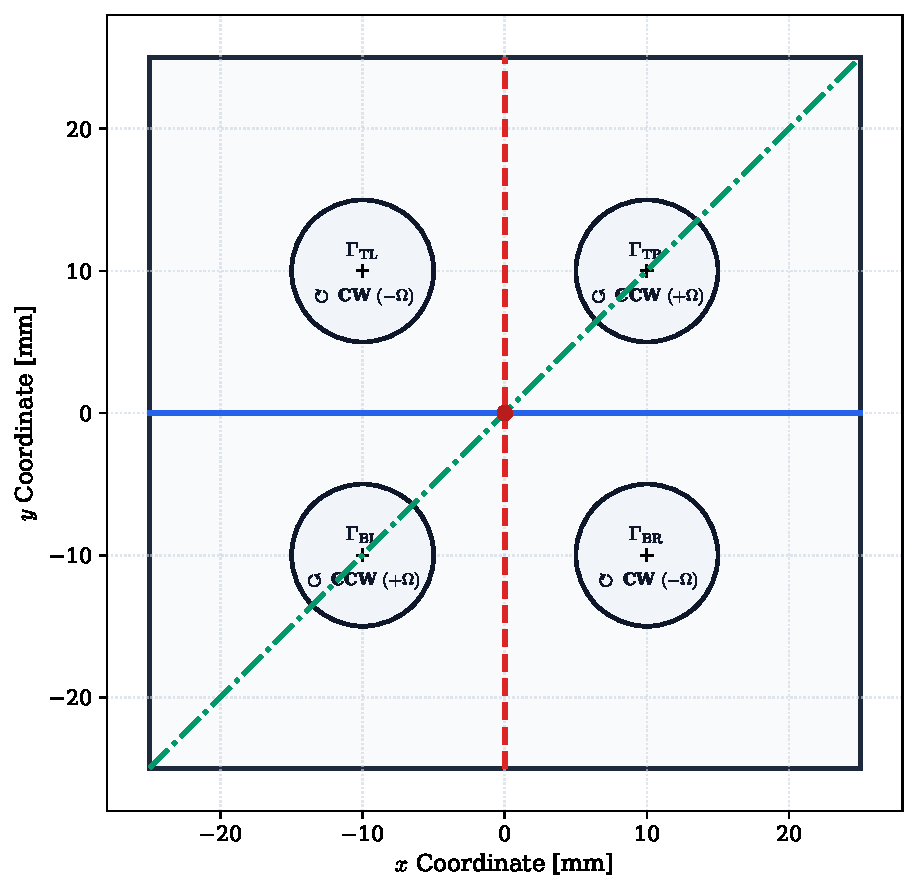
\includegraphics[width=0.68\linewidth]{media/four_roll_cutlines_schema.pdf}
    \caption{Schematic of the four-roll mill geometry with the four
    counter-rotating cylinders, central extensional stagnation point $(0,0)$ (red
    circle), and three diagnostic verification cutlines:
    Horizontal ($y=0$, outflow, blue solid), Vertical ($x=0$, inflow, red dashed),
    and Oblique Diagonal ($y=x$, roller nips, green dash-dot).}
    \label{fig:four_roll_cutlines_schema}
\end{figure}

Figure~\ref{fig:mesh_convergence_cutlines} displays spatial profiles of velocity
and extra-stress tensor components ($u, v, \tau_{xx}, \tau_{xy}, \tau_{yy}$) across
the cutlines. Spatial velocity profiles between M52k, M88k, and M125k deviate by less
than $0.05\%$, while peak shear stresses in roller gaps differ by under $0.3\%$,
confirming that M125k is fully grid-independent and provides a reliable ground truth.

\begin{figure}[htbp]
    \centering
    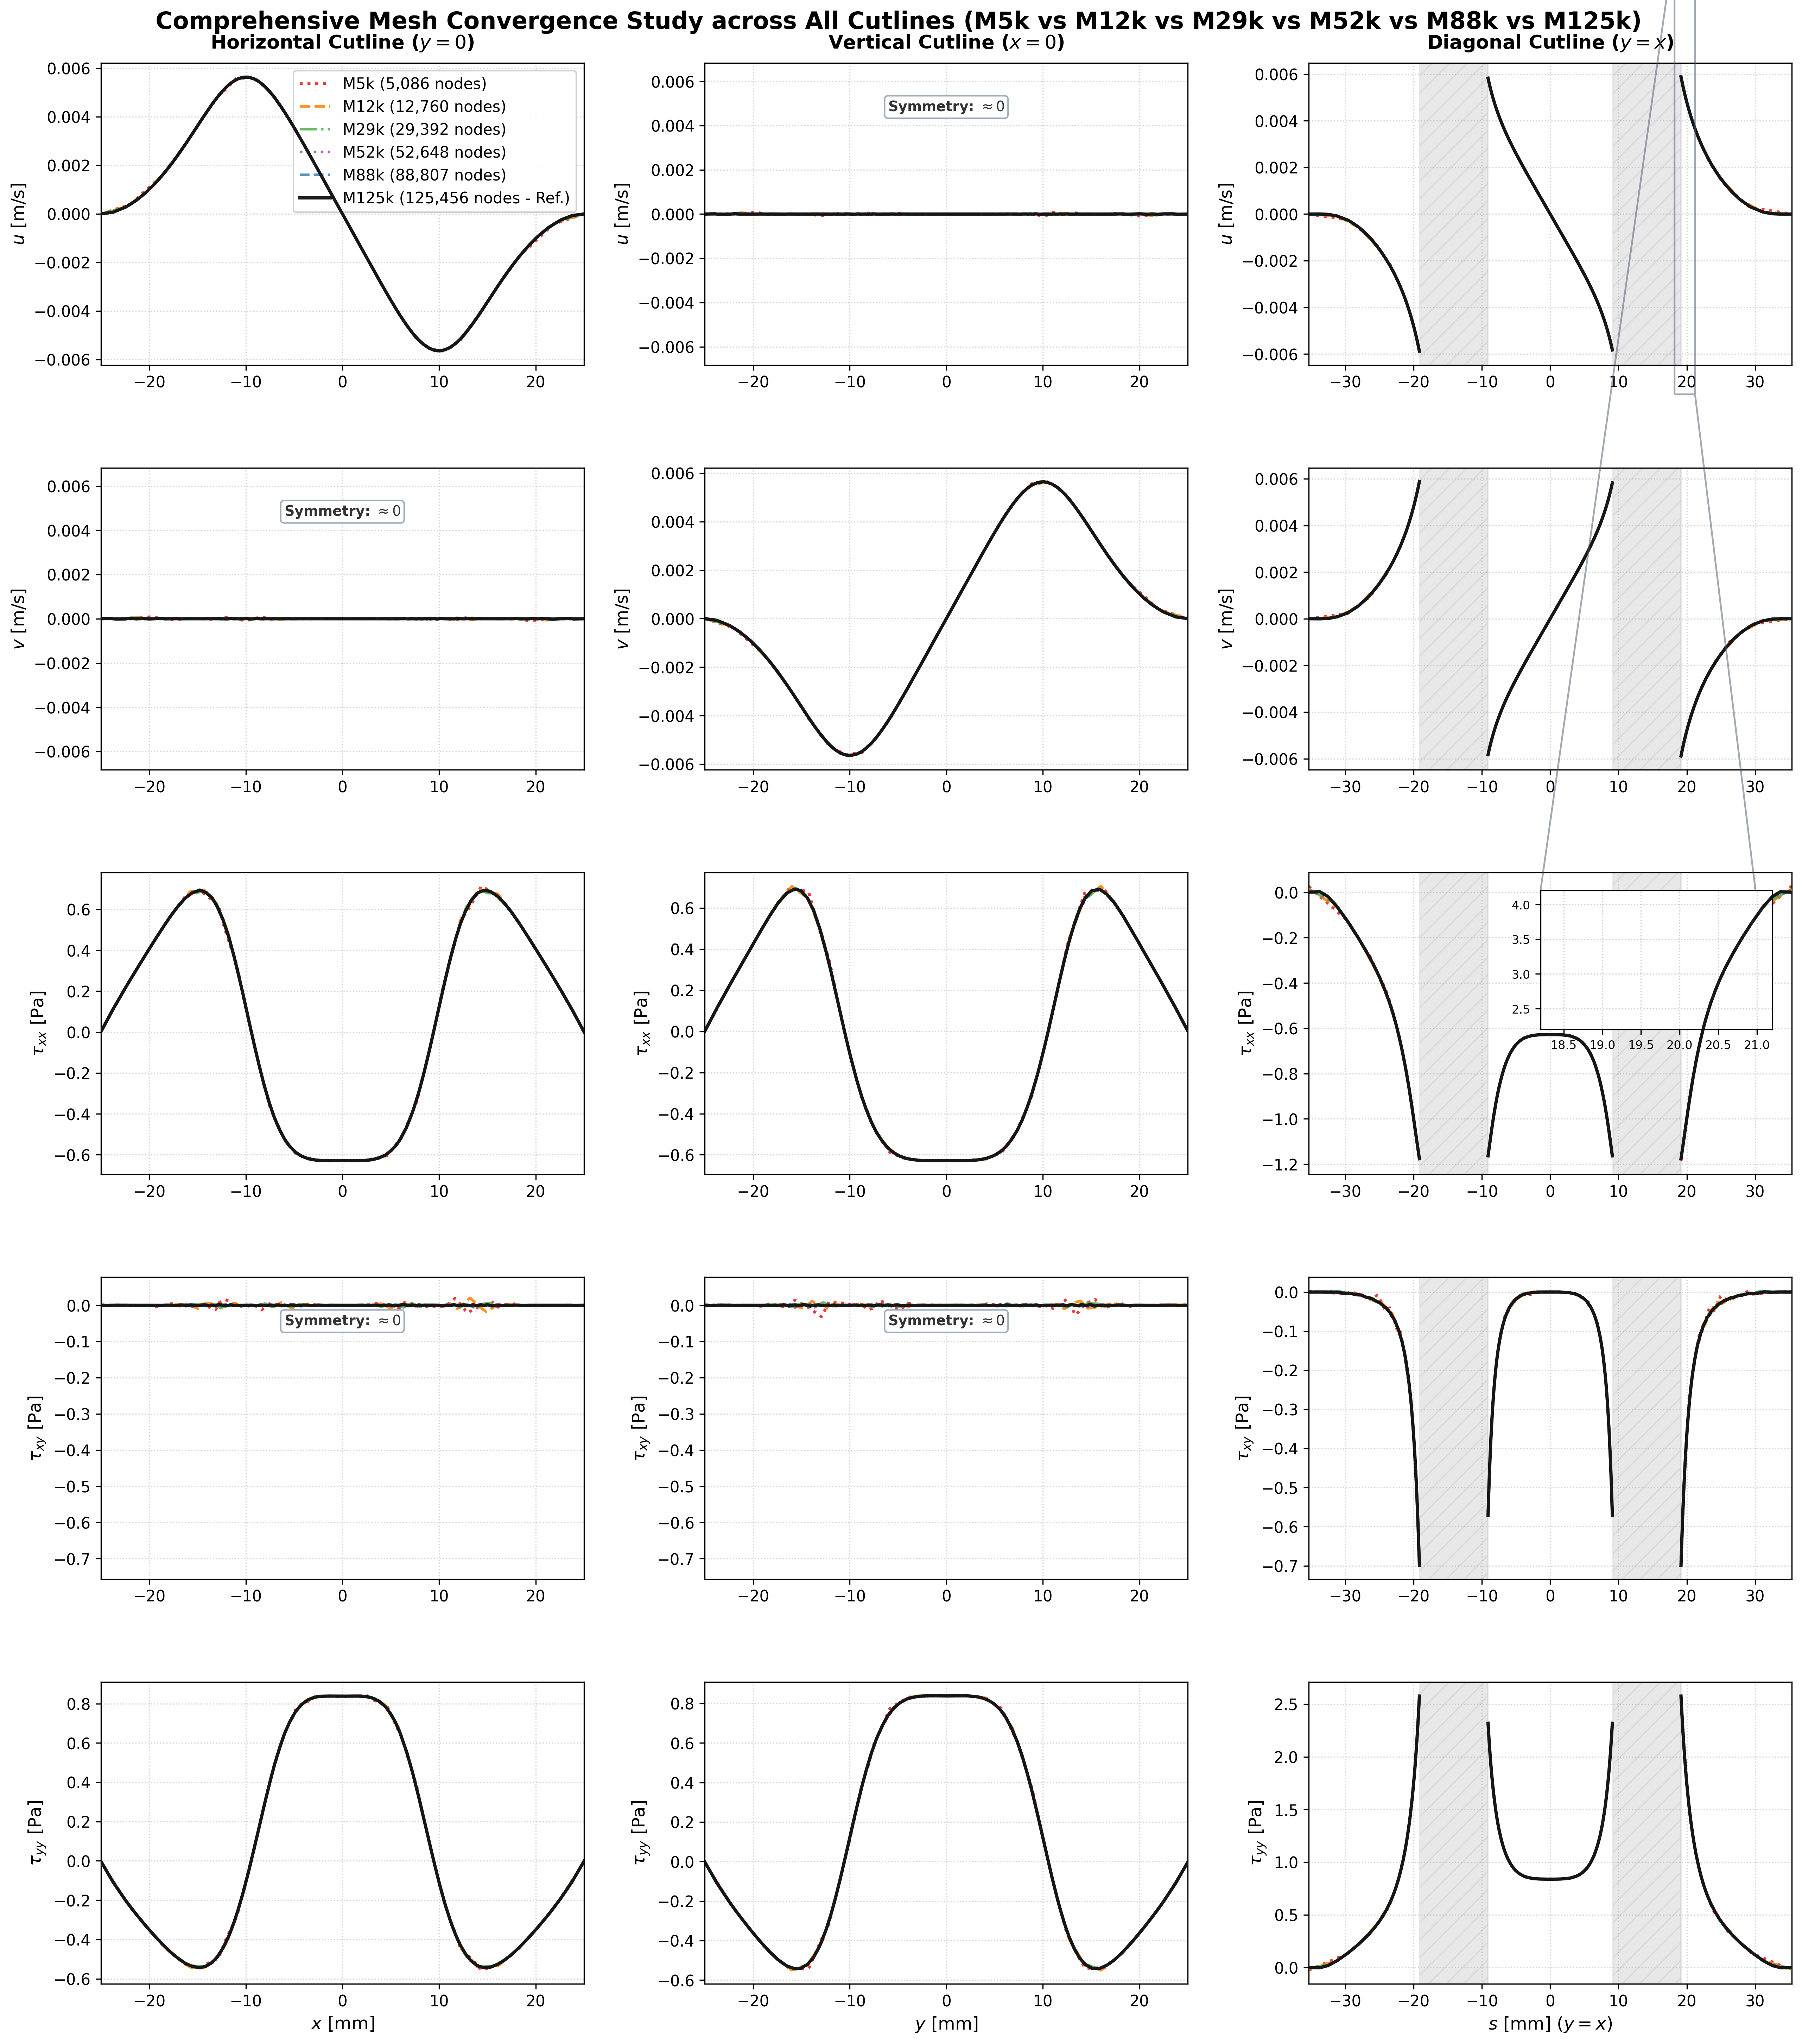
\includegraphics[width=\linewidth]{media/cutlines_convergence_all_fields_matrix.png}
    \caption{High-fidelity COMSOL mesh convergence matrix for the representative
    Oldroyd-B fluid ($\lambda = 1.0\,\mathrm{s}$) across six mesh densities (M5k to
    M125k) along the Horizontal ($y=0$), Vertical ($x=0$), and Oblique Diagonal
    ($y=x$) cutlines for velocity components $(u, v)$ and stress tensor components
    $(\tau_{xx}, \tau_{xy}, \tau_{yy})$. Shaded gray vertical bands in the diagonal
    cutline panels indicate the solid interior occupied by the cylindrical rollers.}
    \label{fig:mesh_convergence_cutlines}
\end{figure}

% ============================================================
% 4.3 NETWORK ARCHITECTURE AND LOSS FORMULATION
% ============================================================
\section{Network Architecture and Loss Formulation}
\label{sec:network_architecture_loss}

\subsection{Decoupled Three-Head Network}
\label{subsec:decoupled_three_head_architecture}

Following the stream function formulation introduced in Section~\ref{subsec:stream_function_formulation}
(Eq.~\eqref{eq:stream_function_def}), the velocity field identically satisfies
mass conservation ($\nabla \cdot \boldsymbol{u} \equiv 0$).
As shown in Figure~\ref{fig:pinn_three_head_architecture}, the physical fields
are predicted by three independent Multi-Layer Perceptron (MLP) branches rather
than a single shared network:
\begin{equation}
    (x, y) \longrightarrow 
    \begin{cases}
        \psi(x, y)  & \text{(Stream function, yielding } u, v\text{ via AD)}, \\
        p(x, y) & \text{(Hydrodynamic pressure)}, \\
        \boldsymbol{\tau}(x, y) = (\tau_{xx}, \tau_{xy}, \tau_{yy}) & \text{(Extra-stress tensor)} .
    \end{cases}
    \label{eq:three_heads_mapping}
\end{equation}
Each branch contains 8 hidden layers with 128 neurons per layer, activated by
the Sigmoid Linear Unit ($\mathrm{SiLU}(z) = z / (1 + e^{-z})$). Its smooth,
infinitely differentiable profile provides well-behaved second and third-order
derivative graphs during automatic differentiation.

\begin{figure}[htbp]
    \centering
    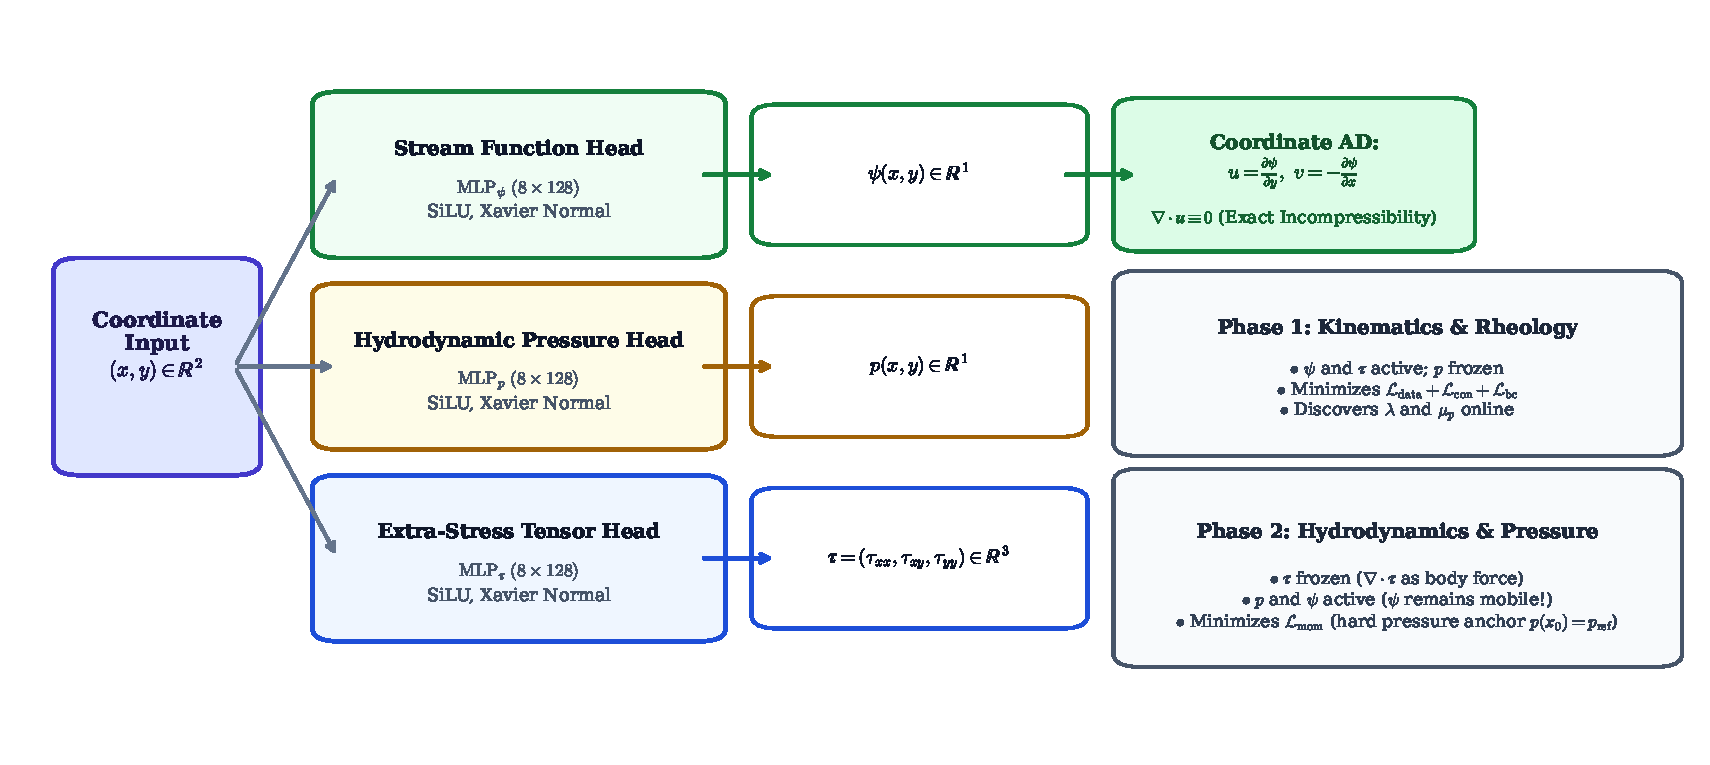
\includegraphics[width=0.95\linewidth]{media/pinn_three_head_architecture.pdf}
    \caption{Decoupled three-head neural network architecture for the
    viscoelastic four-roll mill solver, showing coordinate inputs, separate MLP heads
    for stream function $\psi$, pressure $p$, and stress tensor $\boldsymbol{\tau}$,
    coordinate automatic differentiation, and the two-stage optimization schedule.}
    \label{fig:pinn_three_head_architecture}
\end{figure}

\subsection{Weight Initialization}
\label{subsec:physics_informed_initialization}

Hidden layers are initialized with the Xavier normal distribution, scaling
weight variance inversely with layer width to maintain balanced gradient
amplitudes across depth.

The final linear layers of the extra-stress network $\mathcal{N}_{\boldsymbol{\tau}}$
and pressure network $\mathcal{N}_p$ are initialized to zero
($\boldsymbol{W}^{(L)} = \boldsymbol{0}, \boldsymbol{b}^{(L)} = \boldsymbol{0}$).
This choice provides two practical benefits:
\begin{enumerate}
    \item \textbf{Better Starting State}:
        At iteration zero, the model predicts zero extra-stress
        ($\boldsymbol{\tau} = \boldsymbol{0}$) and uniform pressure, reflecting
        a fluid initially at rest before deformation begins.
    \item \textbf{Numerical Stability}:
        Random initial weights in the stress network produce high-frequency
        spatial fluctuations. Because constitutive models contain nonlinear
        terms ($\alpha \boldsymbol{\tau}^2$ in Giesekus) and convective terms
        ($\boldsymbol{u} \cdot \nabla \boldsymbol{\tau}$), uncalibrated stresses
        at step zero can generate extreme loss spikes ($> 10^6$) that disrupt
        the optimizer. Initializing output layers to zero avoids these early
        instabilities.
\end{enumerate}

\subsection{Governing Residuals and Scaling}
\label{subsec:governing_residuals_scaling}

Following the nondimensionalization introduced in Section~\ref{sec:nondimensionalization},
characteristic scales are $H_{\mathrm{ref}} = R = 0.005\,\mathrm{m}$ (roller radius)
and $U_{\mathrm{ref}} = u_{\mathrm{roll}} = 8.333 \times 10^{-3}\,\mathrm{m/s}$.
In the inverse problem, fluid viscosities $\mu_s$ and $\mu_p$ are unknown a priori.
To decouple the coordinate scaling from evolving parameter estimates, the solver
sets a fixed reference viscosity scale $\eta_0 = 1.0\,\mathrm{Pa\cdot s}$:
\begin{equation}
    \mu_s^* = \frac{\mu_s}{\eta_0}, \quad \mu_p^* = \frac{\mu_p}{\eta_0}, \quad Re_{\mathrm{scale}} = 
    \frac{\rho U_{\mathrm{ref}} H_{\mathrm{ref}}}{\eta_0}, \quad Wi = \frac{\lambda U_{\mathrm{ref}}}{H_{\mathrm{ref}}} .
    \label{eq:nondim_scaling_implementation}
\end{equation}

Spatial coordinates are mapped to the unit box $[0, 1]^2$ using the cavity width
$H_{\mathrm{coord}} = L = 0.05\,\mathrm{m}$ to keep activation arguments well
conditioned. Derivative operators with respect to physical space are scaled
accordingly via Automatic Differentiation by $(H_{\mathrm{ref}} / H_{\mathrm{coord}})$.

In contrast to the coordinates, the physical output fields ($p$ and stress
components $\tau_{xx}, \tau_{xy}, \tau_{yy}$) oscillate symmetrically with both
positive and negative values across the cavity. To keep raw network outputs in
the balanced range $[-1, 1]$, each output head is scaled by its maximum absolute
reference value ($p_{\mathrm{scale}}, \boldsymbol{\tau}_{\mathrm{scale}}$):
\begin{equation}
    p(x, y) = p_{\mathrm{scale}} \cdot \hat{p}(x, y), \qquad \boldsymbol{\tau}(x, y) = \boldsymbol{\tau}_{\mathrm{scale}}
    \cdot \hat{\boldsymbol{\tau}}(x, y) ,
    \label{eq:output_scaling_vectors}
\end{equation}
where $\hat{p}, \hat{\boldsymbol{\tau}} \in [-1, 1]$ are the normalized network
outputs. Hereafter, denoting the dimensionless reconstructed physical fields
scaled by the characteristic reference quantities of
Section~\ref{subsec:dimensionless_vector_system} simply as $(u, v, p, \boldsymbol{\tau})$,
the governing PDE residuals evaluated at interior collocation points
$\boldsymbol{x}_m \in \Omega$ evaluate to:
\begin{enumerate}
    \item \textbf{Linear Momentum Residuals} ($f_u, f_v$):
    \begin{align}
        f_u &= Re_{\mathrm{scale}} \left( u \frac{\partial u}{\partial x} + v \frac{\partial u}{\partial y} \right) + \frac{\partial p}{\partial x} - \mu_s^* \left( \frac{\partial^2 u}{\partial x^2} + \frac{\partial^2 u}{\partial y^2} \right) - \left( \frac{\partial \tau_{xx}}{\partial x} + \frac{\partial \tau_{xy}}{\partial y} \right) , \label{eq:residual_fu_explicit} \\
        f_v &= Re_{\mathrm{scale}} \left( u \frac{\partial v}{\partial x} + v \frac{\partial v}{\partial y} \right) + \frac{\partial p}{\partial y} - \mu_s^* \left( \frac{\partial^2 v}{\partial x^2} + \frac{\partial^2 v}{\partial y^2} \right) - \left( \frac{\partial \tau_{xy}}{\partial x} + \frac{\partial \tau_{yy}}{\partial y} \right) . \label{eq:residual_fv_explicit}
    \end{align}
    \item \textbf{Viscoelastic Constitutive Residuals}
        ($f_{\tau_{xx}}, f_{\tau_{xy}}, f_{\tau_{yy}}$):
    \begin{align}
        f_{\tau_{xx}} &= \mathcal{G}_{xx}(\boldsymbol{\tau}) + Wi \, \overset{\nabla}{\tau}_{xx} - 2\mu_p^* \frac{\partial u}{\partial x} , \label{eq:residual_ftxx_explicit} \\
        f_{\tau_{yy}} &= \mathcal{G}_{yy}(\boldsymbol{\tau}) + Wi \, \overset{\nabla}{\tau}_{yy} - 2\mu_p^* \frac{\partial v}{\partial y} , \label{eq:residual_ftyy_explicit} \\
        f_{\tau_{xy}} &= \mathcal{G}_{xy}(\boldsymbol{\tau}) + Wi \, \overset{\nabla}{\tau}_{xy} - \mu_p^* \left( \frac{\partial u}{\partial y} + \frac{\partial v}{\partial x} \right) , \label{eq:residual_ftxy_explicit}
    \end{align}
    where $\overset{\nabla}{\tau}_{ij}$ denotes the upper-convected derivative
    (Eq.~\eqref{eq:uctd_definition}), and $\boldsymbol{\mathcal{G}}(\boldsymbol{\tau})$
    defines the constitutive model:
    \begin{equation}
        \boldsymbol{\mathcal{G}}(\boldsymbol{\tau}) = 
        \begin{cases}
            \boldsymbol{\tau} & \text{(Oldroyd-B)}, \\[1ex]
            \boldsymbol{\tau} + \dfrac{\alpha Wi}{\mu_p^*} \boldsymbol{\tau}^2 & \text{(Giesekus)}, \\[1ex]
            \left(1 + \dfrac{\varepsilon Wi}{\mu_p^*} \text{tr}(\boldsymbol{\tau})\right) \boldsymbol{\tau} & \text{(Linear PTT)} .
        \end{cases}
        \label{eq:unified_constitutive_cases}
    \end{equation}
\end{enumerate}

\subsection{Loss Formulation}
\label{subsec:multiobjective_loss_formulation}

The composite objective function minimized during training is:
\begin{equation}
    \mathcal{L}_{\mathrm{total}} = w_{\mathrm{data}} \mathcal{L}_{\mathrm{data}} + w_{\mathrm{bc}} \mathcal{L}_{\mathrm{bc}} + w_{\mathrm{con}} \mathcal{L}_{\mathrm{con}} + w_{\mathrm{mom}} \mathcal{L}_{\mathrm{mom}} + w_{\mathrm{roll\_stress}} \mathcal{L}_{\mathrm{roll\_stress}} .
    \label{eq:composite_loss_detailed}
\end{equation}
Because spatial coordinates ($[0, 1]^2$), kinematic velocities ($\mathcal{O}(1)$ via
$U_{\mathrm{ref}}$ and variance scaling), and stress/pressure outputs are systematically
scaled to dimensionless order-unity values, the individual loss components remain
naturally balanced without requiring stiff empirical weighting.
Accordingly, the baseline weights are set uniformly to unity:
$w_{\mathrm{data}} = 1.0$, $w_{\mathrm{bc}} = 1.0$, and $w_{\mathrm{con}} = 1.0$.
The momentum balance weight follows the staged training schedule ($w_{\mathrm{mom}} = 0.0$
in Phase~1, $w_{\mathrm{mom}} = 1.0$ in Phase~2), while $w_{\mathrm{roll\_stress}} = 1.0$
is selectively activated during inverse parameter discovery and disabled
($w_{\mathrm{roll\_stress}} = 0$) during direct field reconstruction.

The individual loss terms are defined as follows:
\begin{itemize}
    \item \textbf{Kinematic Data Loss} ($\mathcal{L}_{\mathrm{data}}$):
        Quantifies the mean squared error against observed dimensionless velocity data:
        \begin{equation}
            \mathcal{L}_{\mathrm{data}} = \frac{1}{N_{\mathrm{data}}} \sum_{i=1}^{N_{\mathrm{data}}} \left[ \frac{(\hat{u}(\boldsymbol{x}_i) - u_i^{\mathrm{data}})^2}{\sigma_u^2} + \frac{(\hat{v}(\boldsymbol{x}_i) - v_i^{\mathrm{data}})^2}{\sigma_v^2} \right] ,
            \label{eq:loss_data_def}
        \end{equation}
        where $\hat{u}(\boldsymbol{x}) = \frac{\partial \hat{\psi}}{\partial y}$,
        $\hat{v}(\boldsymbol{x}) = -\frac{\partial \hat{\psi}}{\partial x}$,
        and $\sigma_u^2, \sigma_v^2$ are empirical dimensionless field variances
        used to scale horizontal and vertical kinematic errors to comparable magnitude.
    \item \textbf{Kinematic Boundary Loss} ($\mathcal{L}_{\mathrm{bc}}$):
        Enforces no-slip conditions on outer cavity walls and prescribed tangential
        velocities on the rotating cylinder surfaces in dimensionless variables:
        \begin{equation}
            \mathcal{L}_{\mathrm{bc}} = \frac{1}{N_{\mathrm{bc}}} \sum_{j=1}^{N_{\mathrm{bc}}} \left\| \hat{\boldsymbol{u}}(\boldsymbol{x}_j) - \boldsymbol{u}^{\mathrm{wall/roll}}(\boldsymbol{x}_j) \right\|_2^2 .
            \label{eq:loss_bc_def}
        \end{equation}
    \item \textbf{Constitutive Residual Loss} ($\mathcal{L}_{\mathrm{con}}$):
        Evaluates the mean squared residual of the rheological equations over
        collocation points:
        \begin{equation}
            \mathcal{L}_{\mathrm{con}} = \frac{1}{N_{\mathrm{col}}} \sum_{m=1}^{N_{\mathrm{col}}} \left[ f_{\tau_{xx}}(\boldsymbol{x}_m)^2 + f_{\tau_{xy}}(\boldsymbol{x}_m)^2 + f_{\tau_{yy}}(\boldsymbol{x}_m)^2 \right] .
            \label{eq:loss_con_def}
        \end{equation}
    \item \textbf{Momentum Residual Loss} ($\mathcal{L}_{\mathrm{mom}}$):
        Evaluates linear momentum balance over collocation points:
        \begin{equation}
            \mathcal{L}_{\mathrm{mom}} = \frac{1}{N_{\mathrm{col}}} \sum_{m=1}^{N_{\mathrm{col}}} \left[ f_u(\boldsymbol{x}_m)^2 + f_v(\boldsymbol{x}_m)^2 \right] .
            \label{eq:loss_mom_def}
        \end{equation}
    \item \textbf{Pressure Fixing}:
        In incompressible flow with enclosed boundaries, the momentum equations
        determine pressure only through its spatial gradient $\nabla p$.
        Consequently, the absolute hydrostatic level is mathematically indeterminate
        up to an arbitrary additive constant. Rather than imposing a soft penalty
        loss with an empirical weight $w_p$, the pressure sub-network $\mathcal{N}_p$
        is constrained by an exact algebraic hard anchor directly within the forward pass:
        \begin{equation}
            p(\boldsymbol{x}) = p_{\mathrm{scale}} \left( \mathcal{N}_p(\boldsymbol{x}) - \mathcal{N}_p(\boldsymbol{x}_0) \right) + p_{\mathrm{ref}} ,
            \label{eq:pressure_hard_anchor_definition}
        \end{equation}
        where $\boldsymbol{x}_0$ denotes a prescribed fixed boundary reference point
        (selected on the external wall) and $p_{\mathrm{ref}}$ is the corresponding
        reference Dirichlet value. This construction identically guarantees
        $p(\boldsymbol{x}_0) \equiv p_{\mathrm{ref}}$ for all network parameters
        $\boldsymbol{\theta}_p$, acting as an exact single-point Dirichlet gauge
        without introducing competing loss terms or gradient conflicts.
\end{itemize}

\subsection{Roller Stress Supervision}
\label{subsec:roller_stress_anchor}

In inverse discovery mode, extra-stress observations are restricted exclusively
to the rotating cylinder boundaries $\Gamma_{\mathrm{roll}}$:
\begin{equation}
    \mathcal{L}_{\mathrm{roll\_stress}} = \frac{1}{N_{\mathrm{rolls}}} \sum_{k=1}^{N_{\mathrm{rolls}}} \left\| \boldsymbol{\tau}_k - \boldsymbol{\tau}_k^{\mathrm{ref}} \right\|_2^2 .
    \label{eq:loss_roll_stress_definition}
\end{equation}
This localized boundary condition provides a necessary reference to anchor the
stress scale and couple kinematic fields with the constitutive relations during
parameter inversion, without requiring any stress measurements inside the fluid
domain. In the direct problem, where fluid parameters are prescribed, this
supervision term is disabled ($w_{\mathrm{roll\_stress}} = 0$).

% ============================================================
% 4.4 TRAINING STRATEGY
% ============================================================
\section{Training Strategy}
\label{sec:training_strategy}

\subsection{Two-Stage Physical Decoupling}
\label{subsec:two_stage_decoupling_helmholtz}

Optimizing momentum and constitutive equations together from scratch often leads
to numerical instability, causing the optimizer to stall or produce unphysical fields.

To avoid this imbalance, we split training into two sequential stages:
\begin{enumerate}
    \item \textbf{Phase 1: Kinematics and Rheology (Stress Network Training)}:
        The momentum balance is turned off ($w_{\mathrm{mom}} = 0$) and the
        pressure network $\mathcal{N}_p$ remains frozen. The stream function
        $\psi$ and extra-stress $\boldsymbol{\tau}$ are trained jointly by
        minimizing kinematic data matching alongside constitutive residuals:
        \begin{equation}
            \mathcal{L}_{\text{Phase 1}} = w_{\mathrm{data}} \mathcal{L}_{\mathrm{data}} + w_{\mathrm{bc}} \mathcal{L}_{\mathrm{bc}} + w_{\mathrm{con}} \mathcal{L}_{\mathrm{con}} + w_{\mathrm{roll\_stress}} \mathcal{L}_{\mathrm{roll\_stress}} .
            \label{eq:loss_phase1_formula}
        \end{equation}
        In inverse mode, unknown fluid parameters ($\lambda, \mu_p, \alpha$) are
        identified during this phase, isolating constitutive dynamics from
        hydrodynamic pressure interactions.
    \item \textbf{Phase 2: Hydrodynamics and Pressure Recovery (Momentum Training)}:
        The extra-stress network $\mathcal{N}_{\boldsymbol{\tau}}$ is frozen, and
        its spatial divergence $\nabla \cdot \boldsymbol{\tau}$ is fixed.
        The momentum loss is activated ($w_{\mathrm{mom}} = 1.0$):
        \begin{equation}
            \mathcal{L}_{\text{Phase 2}} = w_{\mathrm{data}} \mathcal{L}_{\mathrm{data}} + w_{\mathrm{bc}} \mathcal{L}_{\mathrm{bc}} + w_{\mathrm{mom}} \mathcal{L}_{\mathrm{mom}} .
            \label{eq:loss_phase2_formula}
        \end{equation}
\end{enumerate}

Crucially, the stream function network $\mathcal{N}_\psi$ remains trainable
alongside $\mathcal{N}_p$ during Phase~2. Keeping $\psi$ mobile allows the
kinematic field to make minor mutual adjustments that reconcile viscous and
elastic forces with the pressure gradient $\nabla p$, avoiding the numerical
stagnation that occurs if the velocity field is rigidly frozen after Phase~1.

Table~\ref{tab:staged_training_summary} summarizes the training stages, active
heads, and loss weights.

\begin{table}[htbp]
    \centering
    \caption{Summary of the decoupled two-stage training strategy.}
    \label{tab:staged_training_summary}
    \resizebox{\textwidth}{!}{%
    \begin{tabular}{lp{3.5cm}p{3.0cm}p{5.5cm}}
        \hline
        \textbf{Stage} & \textbf{Trainable Heads} & \textbf{Frozen Heads} & \textbf{Active Objectives} \\
        \hline
        \textbf{Phase 1} & $\psi, \, \boldsymbol{\tau}$ & $p$ & $\mathcal{L}_{\mathrm{data}} + \mathcal{L}_{\mathrm{bc}} + \mathcal{L}_{\mathrm{con}} + \mathcal{L}_{\mathrm{roll\_stress}}$ \\
        \textbf{Phase 2} & $p, \, \psi$ (mobile) & $\boldsymbol{\tau}$ & $\mathcal{L}_{\mathrm{data}} + \mathcal{L}_{\mathrm{bc}} + \mathcal{L}_{\mathrm{mom}}$ \\
        \hline
    \end{tabular}%
    }
\end{table}

\subsection{Dual-Precision Optimization}
\label{subsec:dual_precision_optimization}

Optimization proceeds in two sequential precision tiers:
\begin{enumerate}
    \item \textbf{Tier 1: Fast Exploration via Adam (FP32)}:
        In early iterations, the loss landscape contains local minima and steep
        gradients. The Adam optimizer runs in single precision (FP32) to take
        advantage of GPU throughput. A cosine annealing schedule
        ($2.5 \times 10^{-3} \to 2.5 \times 10^{-6}$) guides parameter values
        into the attraction basin of the physical solution.
    \item \textbf{Tier 2: Fine-Tuning with L-BFGS in Double Precision (FP64)}:
        To resolve higher-order spatial derivatives without round-off errors and
        eliminate stochastic fluctuations, the model switches to double precision
        (\texttt{torch.float64}). L-BFGS with a Strong Wolfe line search and history
        size $m=50$ provides superlinear convergence, driving PDE residuals down
        to tight numerical tolerances.
\end{enumerate}

\subsection{Transfer Learning}
\label{subsec:transfer_learning_protocol}

Training PINNs from scratch for every fluid regime requires substantial computational
budgets (50{,}000 iterations) and risks local minima at high elasticity.
We establish a Transfer Learning protocol:
\begin{enumerate}
    \item Pre-train the base network on a moderate baseline case
        ($\lambda = 0.05\,\mathrm{s}, Wi = 0.08$).
    \item Transfer pre-trained weights as initializations for target regimes
        characterized by high elasticity ($\lambda = 0.70\,\mathrm{s}, Wi = 1.17$) or
        strong non-linearity ($\alpha = 0.50$).
    \item Fine-tune with halved iteration budgets (25{,}000 iterations), achieving a
        50\% reduction in computational duration while preventing high-$Wi$
        optimization divergence.
\end{enumerate}

Table~\ref{tab:optimization_hyperparameters} details the hyperparameters and
iteration budgets for both precision tiers and initialization strategies.

\begin{table}[htbp]
    \centering
    \caption{Optimization hyperparameters, precision schedule, and transfer learning settings.}
    \label{tab:optimization_hyperparameters}
    \resizebox{\textwidth}{!}{%
    \begin{tabular}{lcccc}
        \hline
        \textbf{Tier} & \textbf{Optimizer} & \textbf{Precision} & \textbf{Iterations (Scratch / TL)} & \textbf{Learning Rate / Line Search} \\
        \hline
        \textbf{Tier 1} & Adam & FP32 & 40{,}000 / 20{,}000 & Cosine Annealing ($2.5\times 10^{-3} \to 2.5\times 10^{-6}$) \\
        \textbf{Tier 2} & L-BFGS & FP64 & 10{,}000 / 5{,}000 & Strong Wolfe ($\alpha_0 = 1.0, \, m = 50$) \\
        \hline
    \end{tabular}%
    }
\end{table}

% ============================================================
% 4.5 DIRECT BENCHMARK: LATENT FIELD RECONSTRUCTION
% ============================================================
\section{Direct Results}
\label{sec:forward_solver_validation}

We evaluate the PINN framework on the Oldroyd-B benchmark
($Wi = 0.0833, Re = 0.0417, \lambda = 0.05\,\mathrm{s}, \mu_p = 0.90\,\mathrm{Pa\cdot s}, \mu_s = 0.10\,\mathrm{Pa\cdot s}$)
under known rheology. Planar velocity observations supervise the stream function
$\hat{\psi}$, while the network autonomously reconstructs the unmeasured latent
extra-stress tensor $\hat{\boldsymbol{\tau}}(x, y)$ and hydrodynamic pressure $\hat{p}(x, y)$
strictly through the momentum and constitutive residuals.

Crucially, the numerical budget allocated to this direct benchmark differs
substantially from the compact schedule adopted for inverse discovery.
While inverse parameter identification is standardized on a compact budget
of 50{,}000 iterations (40{,}000 Adam + 10{,}000 L-BFGS in Phase~1) to evaluate
computational agility and identifiability, the direct benchmark serves to probe the
asymptotic accuracy limit of the multi-head architecture across all physical fields
on the fine 125k grid. Consequently, the forward benchmark employs an extended
two-stage optimization schedule:
\begin{enumerate}
    \item \textbf{Phase~1 (Viscoelastic Stress)}:
        Trained for 150{,}000 Adam iterations (FP32) followed by Phase~1 L-BFGS
        quasi-Newton refinement ($\approx 161{,}500$ cumulative iterations),
        with pressure frozen to cleanly resolve the intense stress boundary layers
        in the roller gaps.
    \item \textbf{Phase~2 (Hydrodynamic Pressure)}:
        Trained for an additional 100{,}000 Adam iterations with momentum residuals
        active ($w_{\mathrm{mom}} = 1.0$) and mobile stream function $\psi$,
        concluded by 10{,}250 L-BFGS iterations (FP64) for high-precision
        pressure gradient reconstruction.
\end{enumerate}
This cumulative investment of over 260{,}000 optimization iterations produces
the reference forward checkpoint (\texttt{checkpoint\_direct\_best\_accuracy\_phase2}),
whose field accuracy metrics are reported in Table~\ref{tab:direct_problem_metrics}.

\subsection{Velocity and Stress}
\label{subsec:kinematic_and_stress_accuracy}

Field accuracy is quantified using the relative global $L_2$ error norm evaluated
over all $N$ nodes:
\begin{equation}
    \epsilon_{L_2}(\phi) = \frac{\|\hat{\phi} - \phi^{\mathrm{ref}}\|_2}{\|\phi^{\mathrm{ref}}\|_2} = \frac{\sqrt{\sum_{i=1}^N |\hat{\phi}(\boldsymbol{x}_i) - \phi^{\mathrm{ref}}(\boldsymbol{x}_i)|^2}}{\sqrt{\sum_{i=1}^N |\phi^{\mathrm{ref}}(\boldsymbol{x}_i)|^2}} .
    \label{eq:error_metrics_definition}
\end{equation}
Complementing the integral $L_2$ norm, local spatial error distributions in contour
maps are reported via the range-relative error:
\begin{equation}
    \epsilon_{\mathrm{range}}(\boldsymbol{x}) = \frac{|\hat{\phi}(\boldsymbol{x}) - \phi^{\mathrm{ref}}(\boldsymbol{x})|}{\max_{\Omega}(\phi^{\mathrm{ref}}) - \min_{\Omega}(\phi^{\mathrm{ref}})} \times 100\% ,
    \label{eq:range_relative_error_definition}
\end{equation}
which normalizes point-wise discrepancies against the full dynamic span of the field.

Table~\ref{tab:direct_problem_metrics} summarizes the validation metrics on the M125k
grid.

\begin{table}[htbp]
    \centering
    \caption{Global hydrodynamic field accuracy for the direct Oldroyd-B benchmark
    ($Wi = 0.0833, Re = 0.0417$) on the M125k evaluation grid (extended schedule:
    150k Adam + L-BFGS Phase~1, followed by 100k Adam + 10k L-BFGS Phase~2).}
    \label{tab:direct_problem_metrics}
    \resizebox{\textwidth}{!}{%
    \begin{tabular}{lccc}
        \hline
        \textbf{Field Variable} & \textbf{Symbol} & \textbf{Relative $L_2$ Error} & \textbf{Physical Assessment} \\
        \hline
        Horizontal Velocity & $u$ & $\mathbf{0.98\%}$ & Outflow jets and four-fold symmetry resolved \\
        Vertical Velocity & $v$ & $\mathbf{0.93\%}$ & Exact incompressibility satisfied via $\psi$ \\
        Shear Extra-Stress & $\tau_{xy}$ & $\mathbf{1.21\%}$ & Localized peak shear in roller nips resolved \\
        Axial Normal Stress & $\tau_{xx}$ & $\mathbf{1.80\%}$ & Elongational stretching along extension axis \\
        Transverse Normal Stress & $\tau_{yy}$ & $\mathbf{1.65\%}$ & Compressive stress along inflow streamlines \\
        Hydrodynamic Pressure & $p$ (1-point anchor) & $\mathbf{18.31\%}$ & Anchored at $\boldsymbol{x}_0$; captures global dynamic topology \\
        \quad \textit{Gauge-calibrated} & $p_{\mathrm{cal}}$ & \textit{8.13\%} & Mean-adjusted to isolate physical gradient $\nabla p$ \\
        \hline
    \end{tabular}%
    }
\end{table}

Figure~\ref{fig:direct_kinematics} compares the predicted dimensionless velocity
components ($u^* = u/U_{\mathrm{ref}}, v^* = v/U_{\mathrm{ref}}$) against the COMSOL
reference ($L_2$ errors of $0.98\%$ for $u$ and $0.93\%$ for $v$, with local range-relative
errors strictly bounded below $3.5\%$). The stream-function parameterization maintains
the four-fold flow symmetry and accurately locates the central hyperbolic stagnation point.

\begin{figure}[htbp]
    \centering
    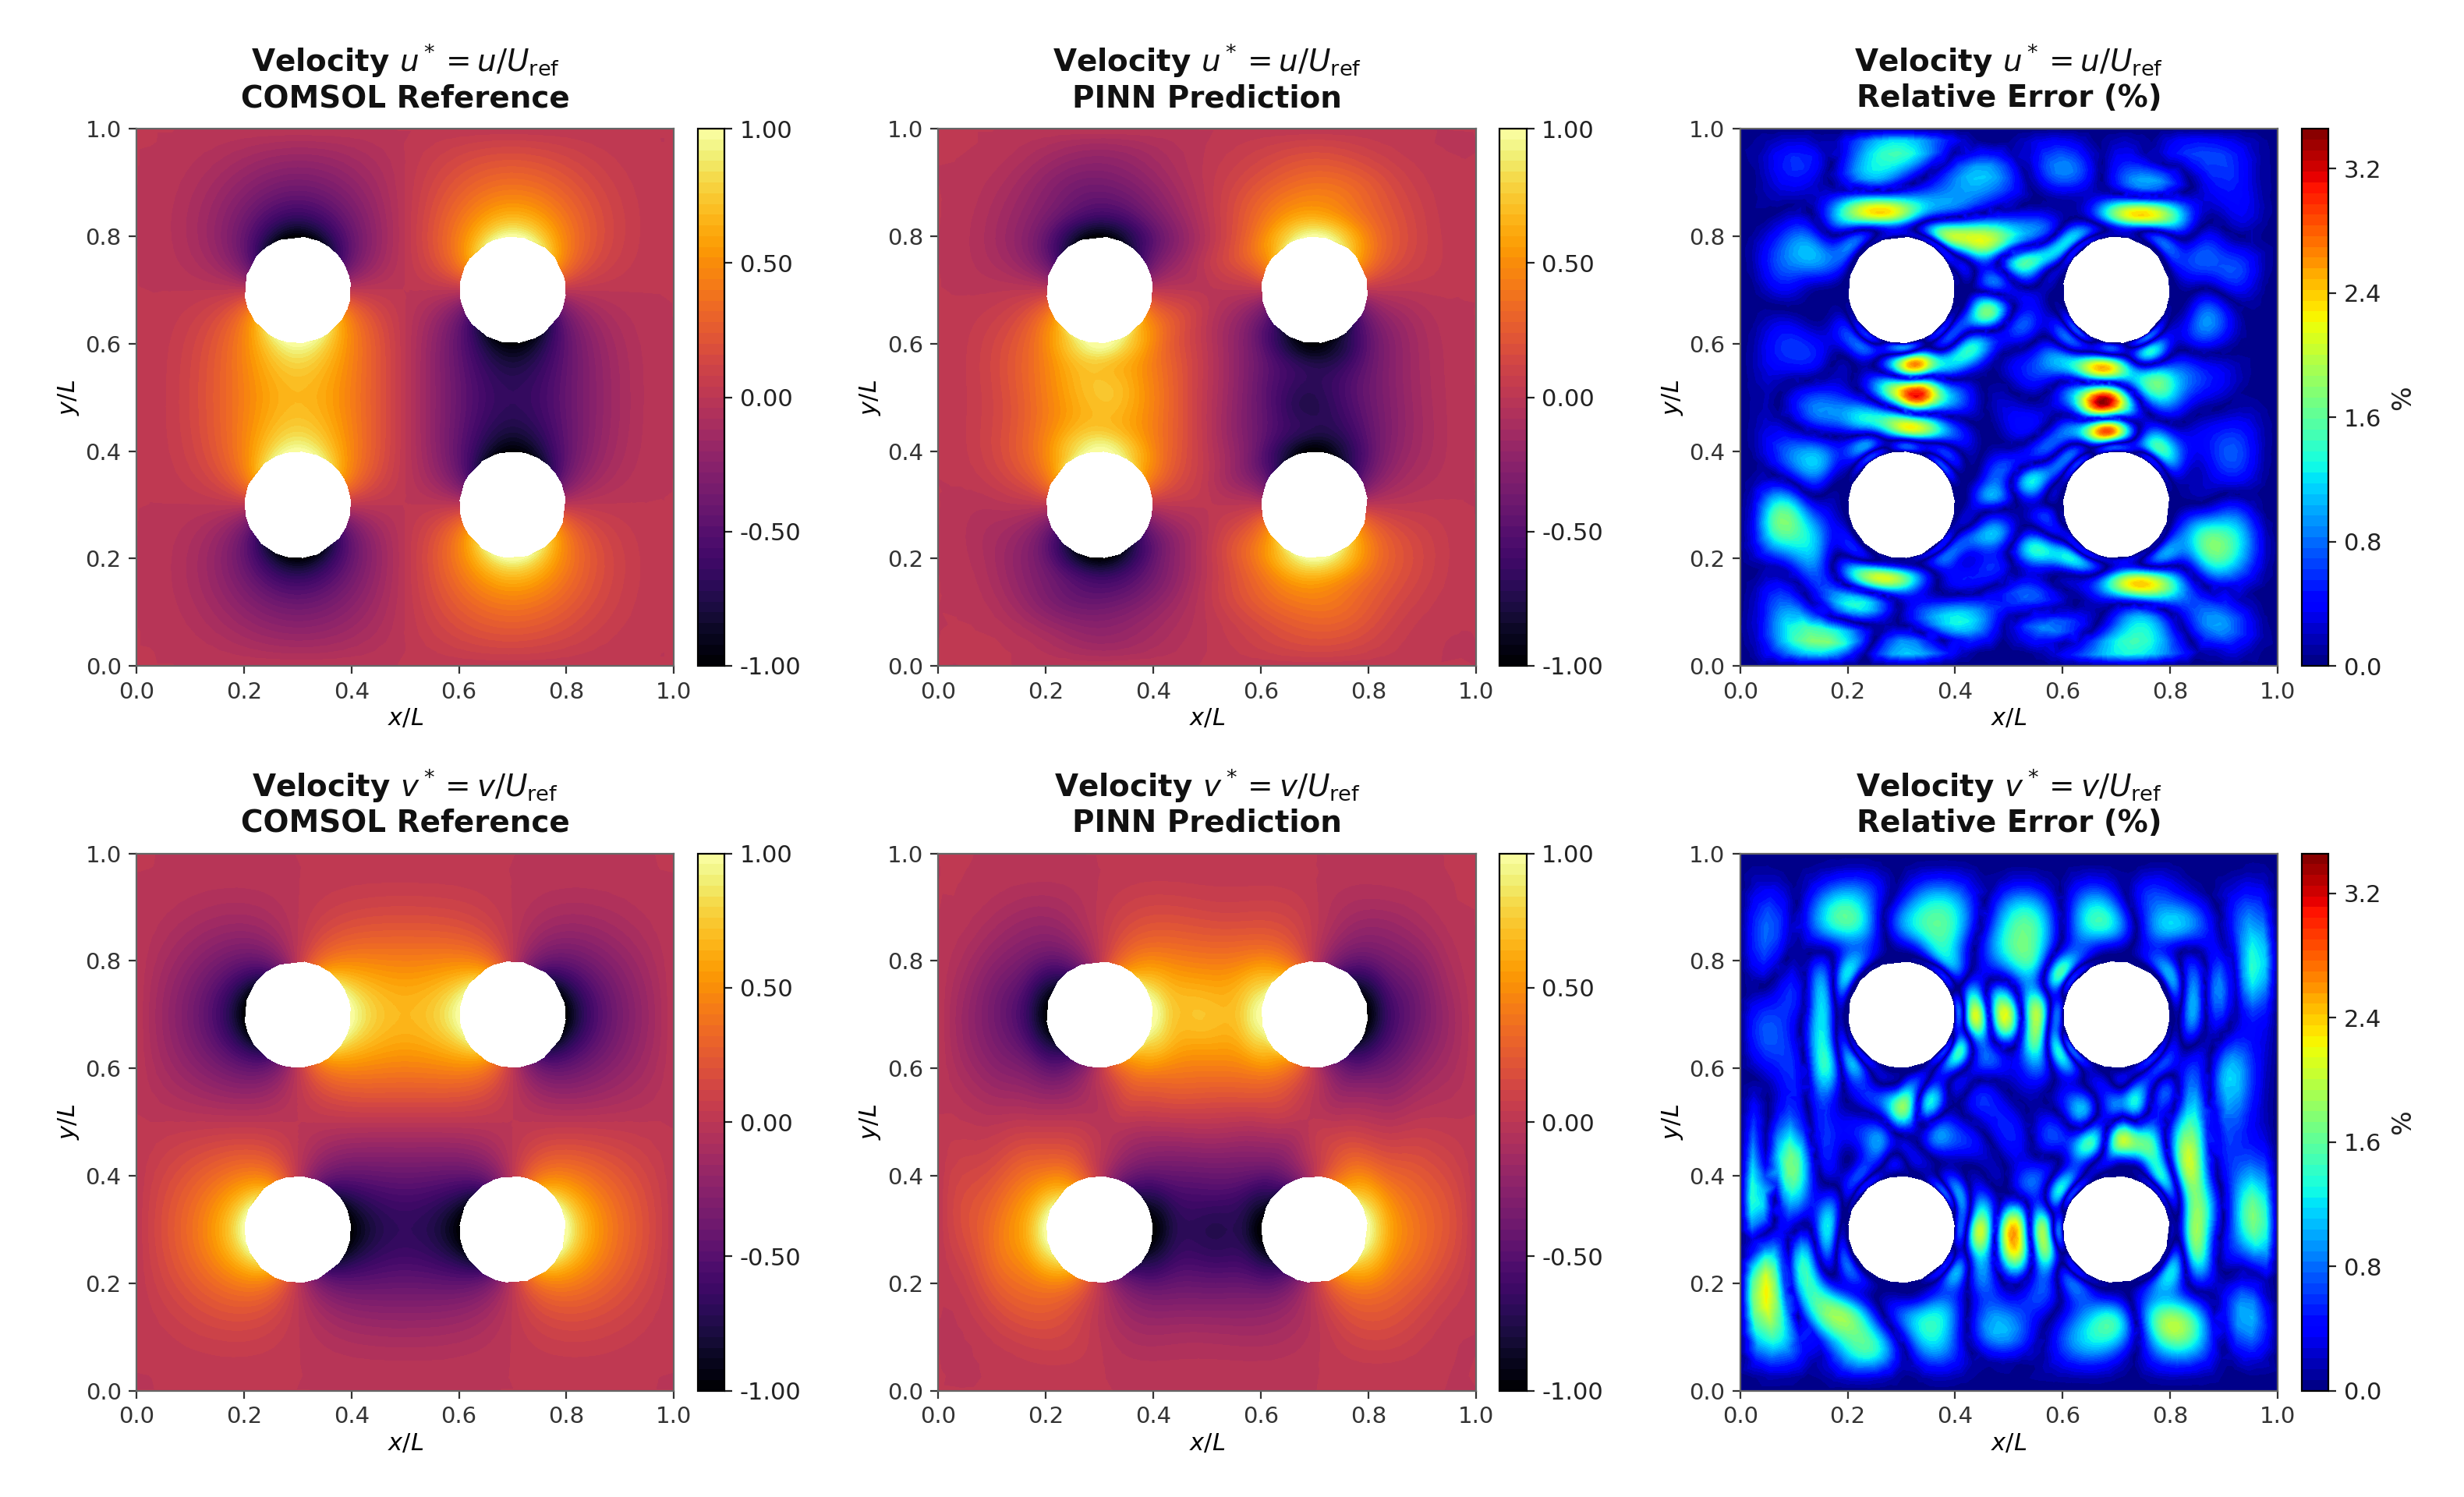
\includegraphics[width=\linewidth]{media/fig1_diretto_cinematica.png}
    \caption{Direct problem kinematic validation: comparison of dimensionless horizontal
    ($u^* = u/U_{\mathrm{ref}}$) and vertical ($v^* = v/U_{\mathrm{ref}}$) velocity fields
    on normalized coordinates $[0, 1]^2$ across COMSOL reference, PINN prediction,
    absolute error, and range-relative error on the M125k mesh.}
    \label{fig:direct_kinematics}
\end{figure}

Figure~\ref{fig:direct_stress} shows the corresponding dimensionless extra-stress
components ($\boldsymbol{\tau}^* = \boldsymbol{\tau}/\tau_{\mathrm{ref}}$), with
relative $L_2$ errors of $1.21\%$ on shear stress $\tau_{xy}^*$ and $1.80\%$ on normal
stress $\tau_{xx}^*$. Stresses are highest in the narrow roller gaps, where intense
velocity shearing occurs, and the network reproduces these localized peaks without
visible numerical oscillations.

\begin{figure}[htbp]
    \centering
    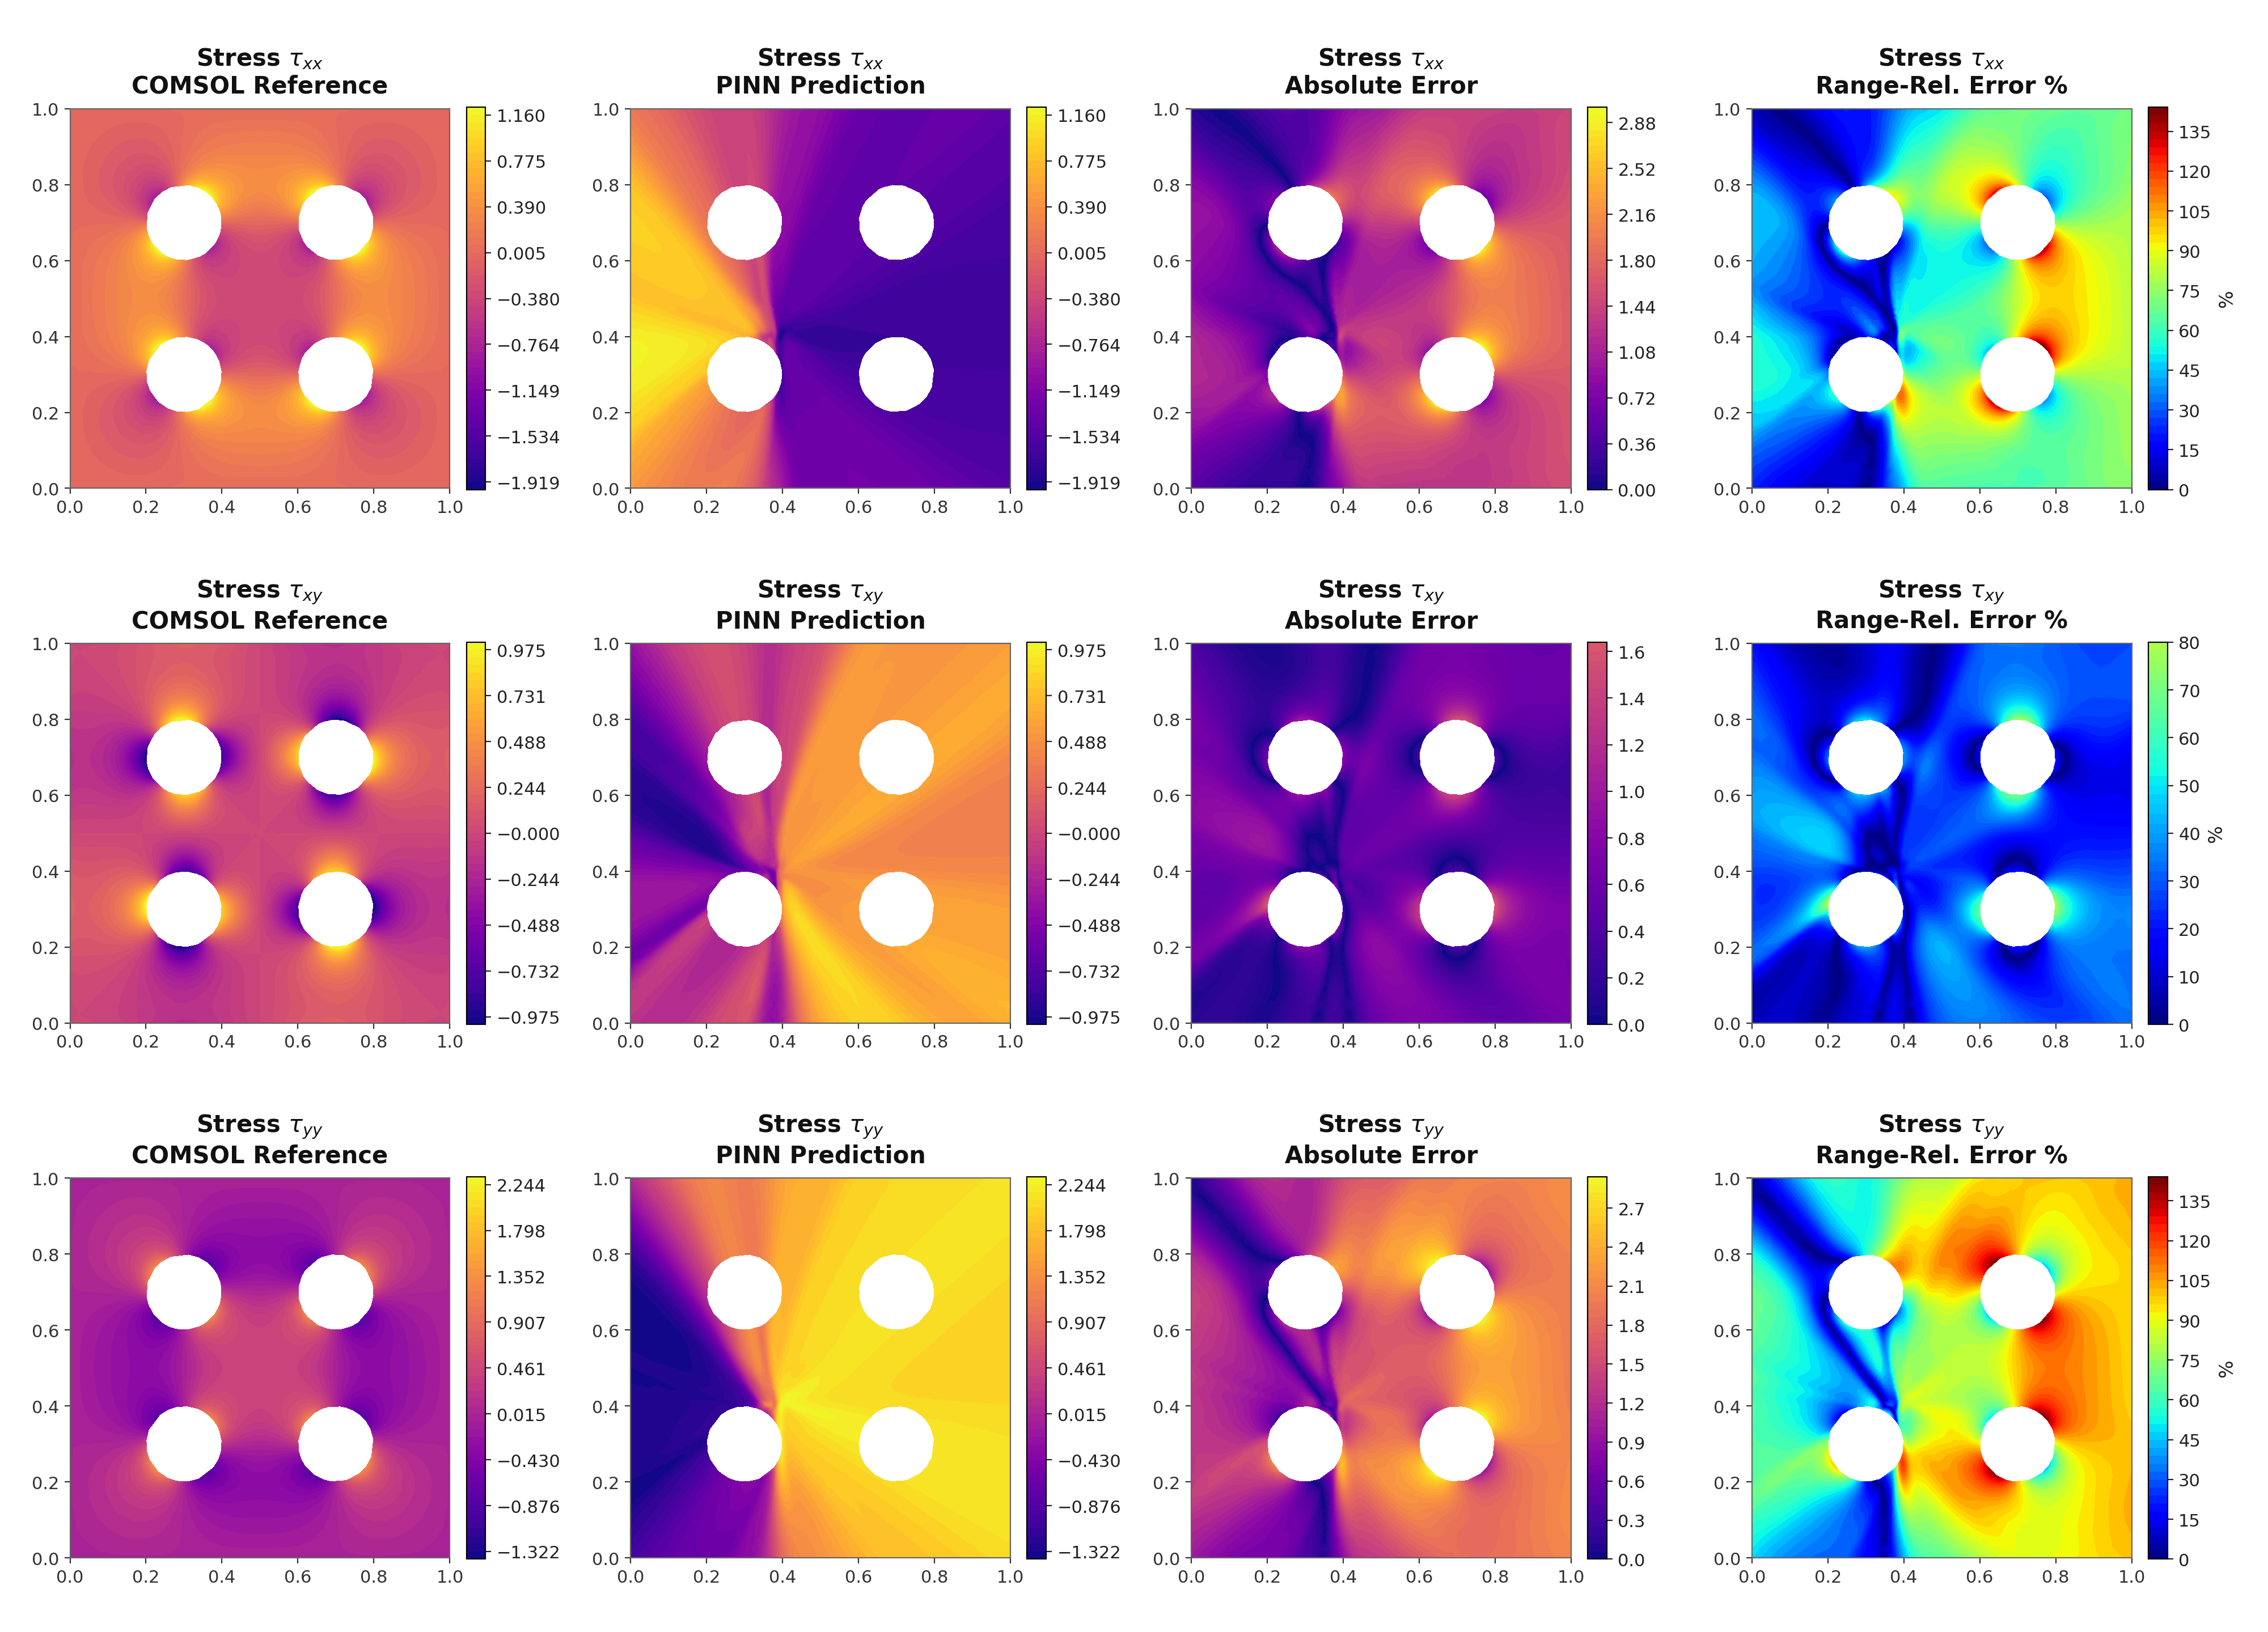
\includegraphics[width=\linewidth]{media/fig3_diretto_stress.png}
    \caption{Direct problem viscoelastic extra-stress tensor validation: dimensionless
    COMSOL ground truth ($\boldsymbol{\tau}^* = \boldsymbol{\tau}/\tau_{\mathrm{ref}}$),
    PINN predictions, absolute errors, and range-relative errors for normal components
    $(\tau_{xx}^*, \tau_{yy}^*)$ and shear component $\tau_{xy}^*$ on normalized
    coordinates $[0, 1]^2$.}
    \label{fig:direct_stress}
\end{figure}

\subsection{Pressure Recovery}
\label{subsec:pressure_recovery_and_calibration}

In an enclosed cavity with prescribed boundary velocities, the momentum equations
determine the pressure field solely through its spatial gradient $\nabla p$.
The absolute hydrostatic level $p$ is therefore determined only up to an arbitrary
additive constant. To eliminate this gauge freedom during training, the network
employs the single-point algebraic hard anchor defined in
Eq.~\eqref{eq:pressure_hard_anchor_definition}, prescribing the reference Dirichlet value
$p(\boldsymbol{x}_0) = p_{\mathrm{ref}}$ at a single external wall node $\boldsymbol{x}_0$.

Figure~\ref{fig:direct_pressure} displays the reconstructed hydrodynamic
pressure field $p^*(\boldsymbol{x}) = p(\boldsymbol{x}) / p_{\mathrm{ref}}$
obtained directly from the network under this single-point boundary anchor.
The PINN accurately resolves the four-fold symmetric hydrodynamic pressure
topology, clearly capturing the local suction troughs in the roller nips
and the central stagnation saddle. Over the entire 125k evaluation mesh, the
reconstructed field achieves a relative $L_2$ error of $18.31\%$, with a mean
range-relative error of $4.08\%$ and a maximum localized error of $13.46\%$.

This $18.31\%$ error represents the realistic operational accuracy of the solver
in practical settings where only a single physical pressure tap is available at
$\boldsymbol{x}_0$. Because the two-dimensional surface is anchored to a single
spatial point on the cavity periphery, any slight residual local discrepancy in
the learned spatial gradient $\nabla p$ accumulates with spatial distance from
$\boldsymbol{x}_0$. Consequently, the reconstructed surface exhibits a slight
global vertical offset relative to the COMSOL reference, elevating the domain-wide
integral $L_2$ norm despite the accurate representation of the underlying flow
dynamics.

\begin{figure}[htbp]
    \centering
    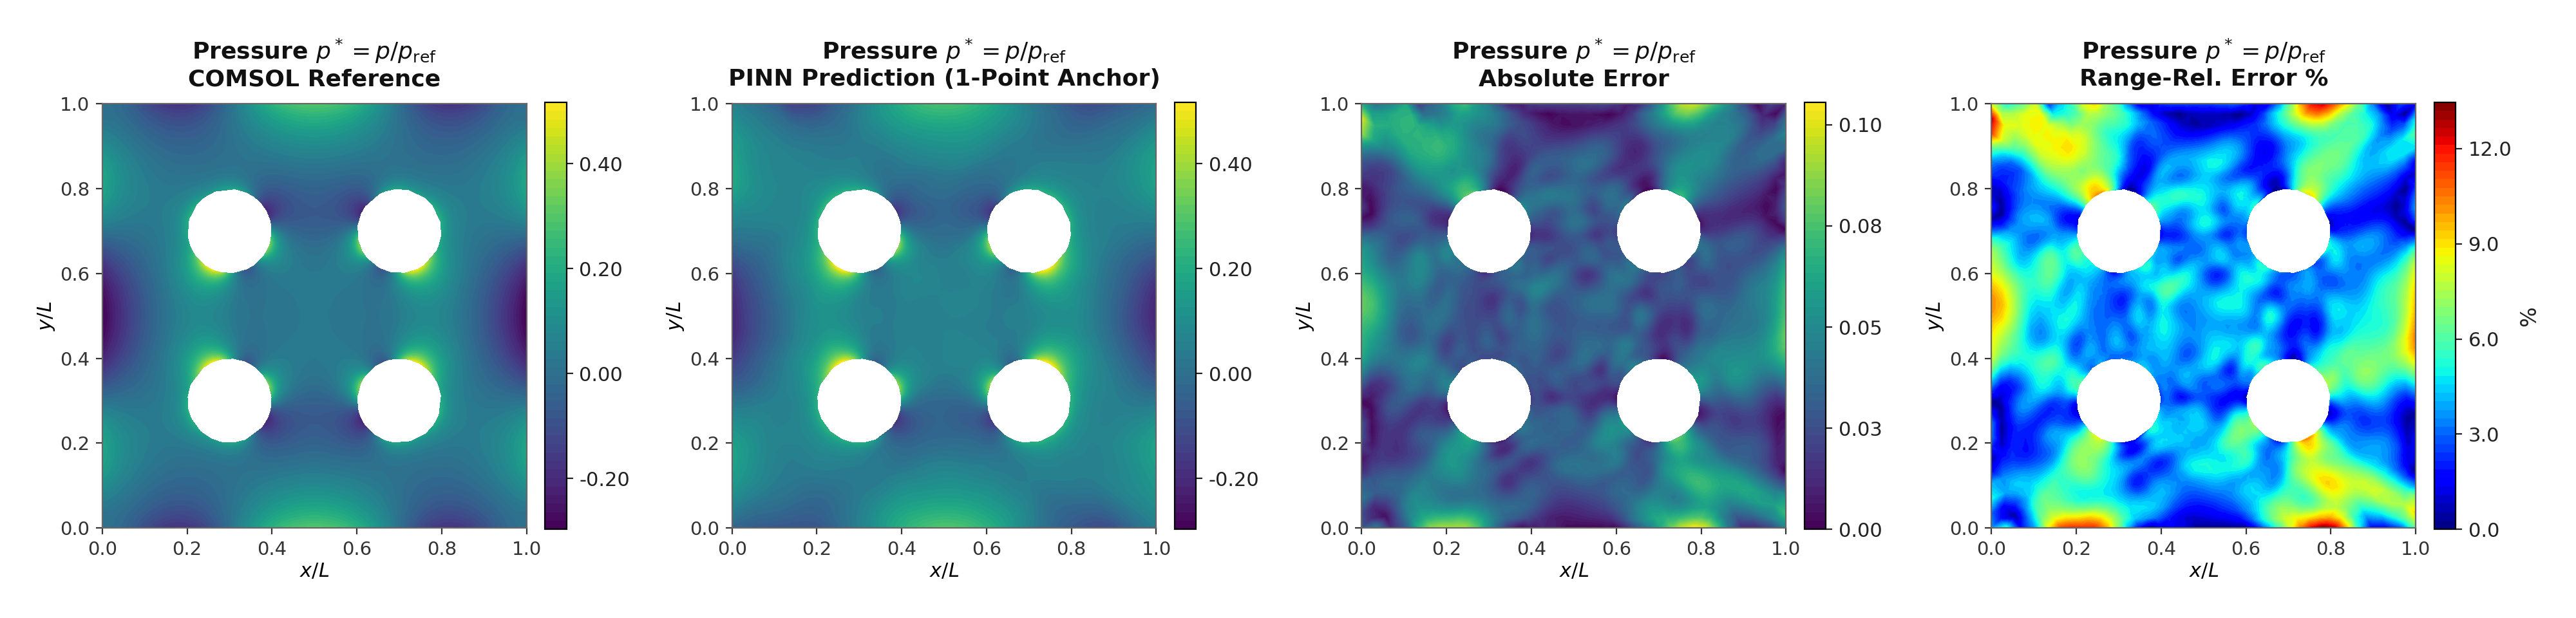
\includegraphics[width=\linewidth]{media/fig2a_diretto_pressione_ancorata.png}
    \caption{Official hydrodynamic pressure field reconstruction under single-point
    algebraic anchoring ($p(\boldsymbol{x}_0) = p_{\mathrm{ref}}$): dimensionless COMSOL ground
    truth ($p^* = p/p_{\mathrm{ref}}$), raw PINN prediction, absolute error, and range-relative
    error distributions on normalized coordinates $[0, 1]^2$ ($L_2$ error of $18.31\%$,
    mean range-relative error of $4.08\%$).}
    \label{fig:direct_pressure}
\end{figure}

============================================================
% 4.6 INVERSE PARAMETER DISCOVERY
% ============================================================
\section{Inverse Parameter Discovery}
\label{sec:inverse_parameter_discovery}

In inverse discovery mode, the PINN operates as a virtual rheometer: no internal
stress measurements are supplied. The network assimilates domain velocity data,
solid boundary kinematic conditions, and the roller stress anchor
($\mathcal{L}_{\mathrm{roll\_stress}}$). Internal stresses and pressure remain
unobserved, inferred simultaneously alongside unknown fluid parameters.

\subsection{Oldroyd-B and Giesekus Benchmarks}
\label{subsec:parameter_discovery_benchmarks}

We evaluate four canonical benchmarks spanning linear Hookean and non-linear
shear-thinning response:
\begin{itemize}
    \item \textbf{Benchmark 1 (Oldroyd-B from Scratch)}:
        Modest elasticity ($Wi = 0.08$), trained ex-novo for 50{,}000 iterations
        starting from blind offset guesses ($\lambda_0 = 0.0535\,\mathrm{s}$ and
        $\mu_p^0 = 0.963\,\mathrm{Pa\cdot s}$, both $+7\%$ from truth).
    \item \textbf{Benchmark 2 (High-Elasticity Oldroyd-B via Transfer Learning)}:
        Elevated elasticity ($Wi = 1.17, \lambda = 0.70\,\mathrm{s}$), fine-tuned via
        TL for 25{,}000 iterations.
    \item \textbf{Benchmark 3 (Non-linear Giesekus with Blind Guess from Scratch)}:
        Non-linear mobility ($\alpha^{\mathrm{true}} = 0.35$), initialized from a
        blind guess $\alpha_0 = 0.25$ and trained for 50{,}000 iterations.
    \item \textbf{Benchmark 4 (Extreme-Mobility Giesekus via Transfer Learning)}:
        Maximum physical mobility
        ($\alpha^{\mathrm{true}} = 0.50, \lambda = 0.30\,\mathrm{s}, \mu_p = 0.05\,\mathrm{Pa\cdot s}$),
        fine-tuned via TL for 25{,}000 iterations.
\end{itemize}

Table~\ref{tab:inverse_benchmarks} summarizes the discovery accuracy and kinematic
errors across these benchmarks.

\begin{table}[htbp]
    \centering
    \caption{Inverse parameter discovery results across the four representative
    benchmarks on the M125k grid.}
    \label{tab:inverse_benchmarks}
    \resizebox{\textwidth}{!}{%
    \begin{tabular}{cllcccc}
        \hline
        \textbf{\#} & \textbf{Model} & \textbf{Strategy} & \textbf{Target Parameter} & \textbf{PINN Estimation} & \textbf{Error} & \textbf{$L_2(u,v)$} \\
        \hline
        \textbf{1} & \textbf{Oldroyd-B} & Ex-Novo & $\lambda = 0.050\,\mathrm{s}$ & $\mathbf{0.0502\,\mathrm{s}}$ & $\mathbf{+0.41\%}$ & \multirow{2}{*}{$0.04\%$} \\
        & ($Wi = 0.08$) & (50k iters) & $\mu_p = 0.900\,\mathrm{Pa\cdot s}$ & $\mathbf{0.9049\,\mathrm{Pa\cdot s}}$ & $\mathbf{+0.54\%}$ & \\
        \hline
        \textbf{2} & \textbf{Oldroyd-B} & Transfer Learning & $\lambda = 0.700\,\mathrm{s}$ & $\mathbf{0.7089\,\mathrm{s}}$ & $\mathbf{+1.27\%}$ & \multirow{2}{*}{$0.33\%$} \\
        & ($Wi = 1.17$) & (25k iters, $-50\%$) & $\mu_p = 0.500\,\mathrm{Pa\cdot s}$ & $\mathbf{0.5019\,\mathrm{Pa\cdot s}}$ & $\mathbf{+0.38\%}$ & \\
        \hline
        \textbf{3} & \textbf{Giesekus} & Ex-Novo (Blind) & $\alpha = 0.350$ & $\mathbf{0.3298}$ & $\mathbf{-5.76\%}$ & \multirow{3}{*}{$0.46\%$} \\
        & ($\alpha_0 = 0.25$) & (50k iters) & $\lambda = 0.100\,\mathrm{s}$ & $\mathbf{0.1032\,\mathrm{s}}$ & $\mathbf{+3.16\%}$ & \\
        & & & $\mu_p = 0.500\,\mathrm{Pa\cdot s}$ & $\mathbf{0.5307\,\mathrm{Pa\cdot s}}$ & $\mathbf{+6.14\%}$ & \\
        \hline
        \textbf{4} & \textbf{Giesekus} & Transfer Learning & $\alpha = 0.500$ & $\mathbf{0.4665}$ & $\mathbf{-6.70\%}$ & \multirow{3}{*}{$0.52\%$} \\
        & (Extreme $\alpha$) & (25k iters, $-50\%$) & $\lambda = 0.300\,\mathrm{s}$ & $\mathbf{0.3077\,\mathrm{s}}$ & $\mathbf{+2.57\%}$ & \\
        & & & $\mu_p = 0.050\,\mathrm{Pa\cdot s}$ & $\mathbf{0.0522\,\mathrm{Pa\cdot s}}$ & $\mathbf{+4.40\%}$ & \\
        \hline
    \end{tabular}%
    }
\end{table}

Parameter estimation errors for Oldroyd-B remain below $1.3\%$ across both low and
high Weissenberg numbers ($Wi = 0.08$ and $Wi = 1.17$). For Giesekus, the solver
simultaneously inverts three coupled parameters $(\alpha, \lambda, \mu_p)$,
identifying mobility $\alpha$ within $6.7\%$ error even from a blind initialization
($\alpha_0 = 0.25$ vs $0.35$).

Figure~\ref{fig:inverse_convergence} illustrates parameter trajectories and objective
function evolution during staged Adam (FP32, initial 40k epochs) and L-BFGS (FP64, final 10k iterations)
optimization on the M125k dataset. In Figure~\ref{fig:inverse_convergence}(left),
the normalized parameter trajectories $\lambda/\lambda_{\mathrm{GT}}$ and
$\mu_p/\mu_{p,\mathrm{GT}}$ initially rise from $1.07$ to an overshoot peak near
$1.28$ during the first 2{,}500 Adam iterations before reversing course and
converging monotonically toward $1.00$. This transient behavior has a direct
physical cause: at iteration zero, the stress network $\mathcal{N}_{\boldsymbol{\tau}}$
is initialized near zero ($\boldsymbol{\tau} \approx \boldsymbol{0}$). In the
absence of a structured stress field, the constitutive residual gradients
momentarily push parameter estimates upward to balance the prescribed deformation
rate. Once the stress head establishes the localized boundary layers and shear
bands (around epoch 3{,}000), the optimizer reorients toward the physical minimum,
guiding parameters into the physical neighborhood. Upon switching to the second-order
L-BFGS optimizer at iteration 40k, the kinematic data loss drops sharply by an
order of magnitude (from $10^{-6}$ to $1.81\times 10^{-7}$), while the constitutive
loss settles monotonically to $\mathcal{L}_{\mathrm{con}} = 6.13\times 10^{-6}$,
providing smooth asymptotic settling without numerical oscillations.

\begin{figure}[htbp]
    \centering
    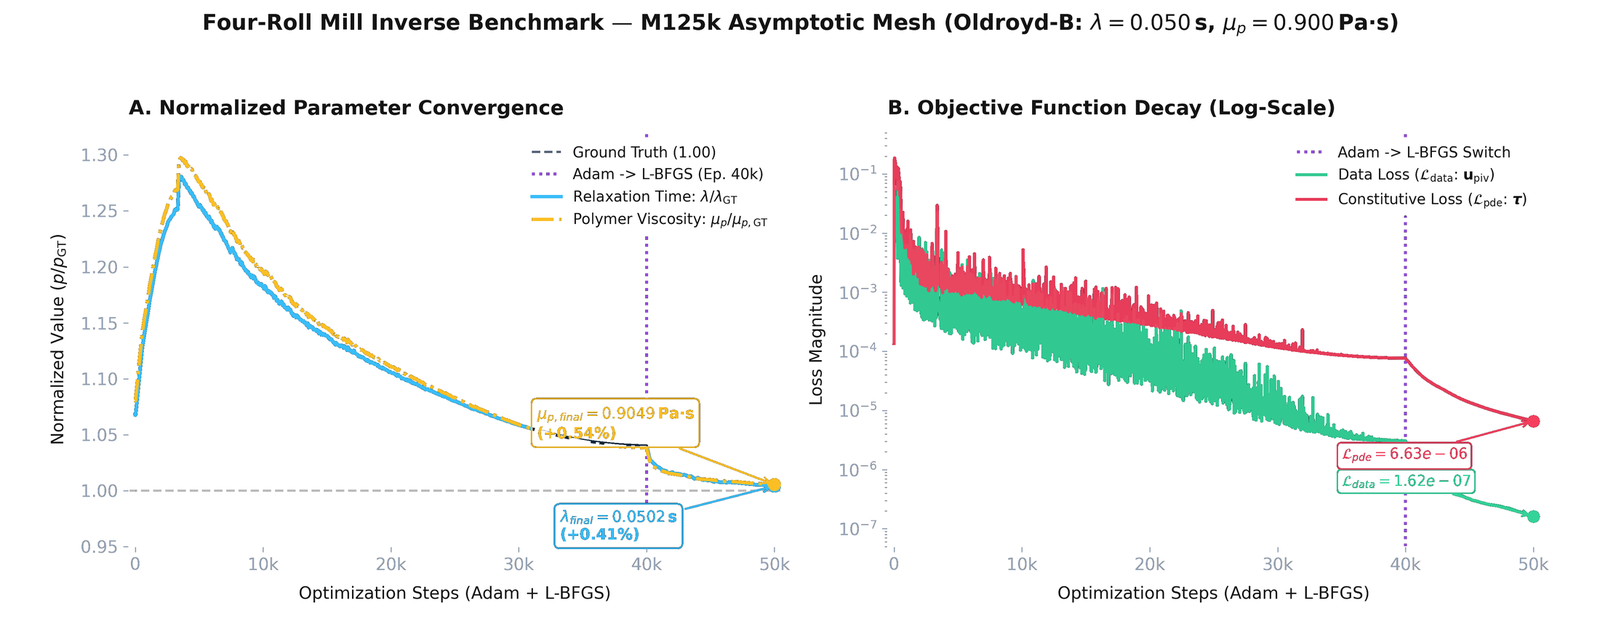
\includegraphics[width=\linewidth]{media/fig4b_inverso_convergence_m125k.png}
    \caption{Parameter convergence trajectories ($\lambda$ and $\mu_p$, left) and
    staged objective loss decay ($\mathcal{L}_{\mathrm{data}}$ and $\mathcal{L}_{\mathrm{con}}$,
    right) during Adam (FP32) and L-BFGS (FP64) optimization on the M125k dataset.}
    \label{fig:inverse_convergence}
\end{figure}

\subsection{Transfer Learning Performance}
\label{subsec:transfer_learning_results}

The benchmarks in Table~\ref{tab:inverse_benchmarks} demonstrate two practical
benefits of transfer learning:
\begin{enumerate}
    \item \textbf{Computational Acceleration}:
        Warm-starting from a pre-trained baseline reduces required iterations by half
        (25{,}000 vs.\ 50{,}000), halving training time.
    \item \textbf{Optimization Regularization}:
        Initializing weights from a lower-$Wi$ solution places the optimization in a
        physically reasonable neighborhood, avoiding the poor local minima that can
        occur when training from scratch at higher elasticity ($Wi = 1.17$) or high
        mobility ($\alpha = 0.50$).
\end{enumerate}

\subsection{Collocation Density Sensitivity}
\label{subsec:collocation_density_sensitivity}

To examine how collocation sampling density affects PINN parameter discovery, we
conducted a systematic grid study across five resolutions from 5k to 125k nodes
(Table~\ref{tab:grid_independence} and Figure~\ref{fig:inverse_mesh_convergence}) on
an Oldroyd-B case ($\lambda = 0.100\,\mathrm{s}, \mu_p = 0.500\,\mathrm{Pa\cdot s}$).

\begin{table}[htbp]
    \centering
    \caption{Collocation density sensitivity and parameter estimation accuracy across
    five resolutions
    ($\lambda^{\mathrm{true}} = 0.100\,\mathrm{s}, \mu_p^{\mathrm{true}} = 0.500\,\mathrm{Pa\cdot s}$).}
    \label{tab:grid_independence}
    \resizebox{\textwidth}{!}{%
    \begin{tabular}{lcccccc}
        \hline
        \textbf{Mesh Resolution} & \textbf{Evaluation Nodes} & $\lambda_{\mathrm{est}}$ [s] & $\lambda$ \textbf{Error} & $\mu_{p,\mathrm{est}}$ [Pa·s] & $\mu_p$ \textbf{Error} & \textbf{Velocity $L_2$} \\
        \hline
        \textbf{5k (Coarse)} & \textbf{5{,}086} & $\mathbf{0.1008}$ & $\mathbf{+0.79\%}$ & $\mathbf{0.5103}$ & $\mathbf{+2.06\%}$ & $\mathbf{0.15\%}$ \\
        \textbf{12k} & 12{,}760 & $0.1071$ & $+7.10\%$ & $0.5389$ & $+7.78\%$ & $0.55\%$ \\
        \textbf{29k} & 29{,}392 & $0.1088$ & $+8.79\%$ & $0.5455$ & $+9.10\%$ & $0.58\%$ \\
        \textbf{52k} & 52{,}648 & $0.1062$ & $+6.18\%$ & $0.5323$ & $+6.46\%$ & $0.44\%$ \\
        \textbf{125k (Dense)} & 125{,}456 & $0.1083$ & $+8.32\%$ & $0.5412$ & $+8.24\%$ & $0.50\%$ \\
        \hline
    \end{tabular}%
    }
\end{table}

\begin{figure}[htbp]
    \centering
    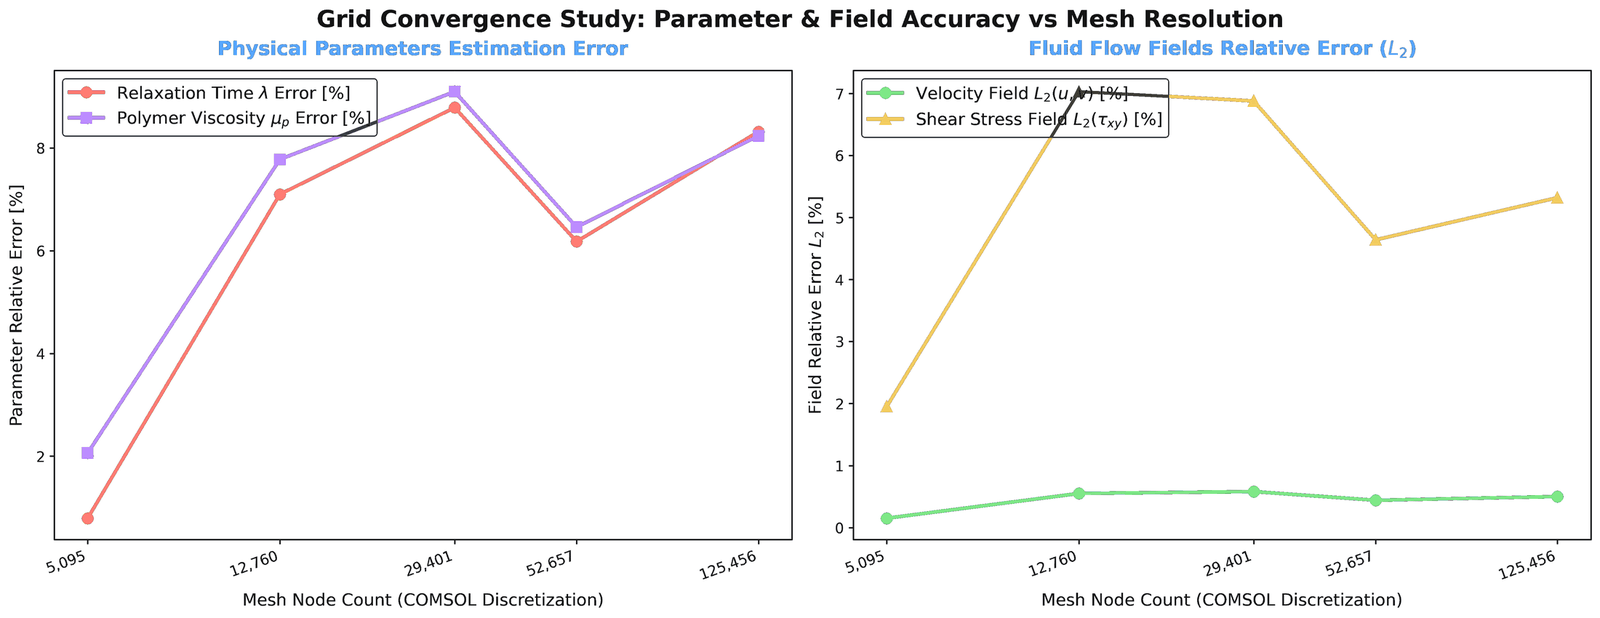
\includegraphics[width=\linewidth]{media/fig5_inverso_mesh_independence.png}
    \caption{Collocation density study: comparison of parameter estimation errors
    ($\lambda$ and $\mu_p$) and velocity $L_2$ errors across resolutions from 5{,}086
    to 125{,}456 collocation points.}
    \label{fig:inverse_mesh_convergence}
\end{figure}

Across a 25-fold variation in collocation point density (from 5{,}086 to
125{,}456 nodes), parameter estimation errors remain consistently bounded
within a narrow interval (${\sim}0.8\%\text{--}8.8\%$), while velocity fields
are reconstructed with high precision ($L_2 \le 0.58\%$).

The modest variations observed across grid resolutions reflect minor random
fluctuations associated with stochastic optimization and spatial collocation
sampling rather than systematic grid-dependent bias. All resolutions yield
comparable, reliable parameter estimates, demonstrating that the inverse solver
is robust to collocation point density and does not require excessively dense
grids to achieve satisfactory convergence.

% ============================================================
% 4.7 IDENTIFIABILITY BOUNDARIES AND INVARIANCE PRINCIPLES
% ============================================================
\section{Limits}
\label{sec:identifiability_limits_degeneracy}

\subsection{Elastic Shear Modulus Invariance}
\label{subsec:preservation_elastic_shear_modulus}

Across all inverse benchmarks, a consistent physical result emerges: while
individual fluid parameters can be sensitive to boundary conditioning, the
\textbf{composite Elastic Shear Modulus} $G = \mu_p / \lambda$ is identified
with high precision across every model tested (Table~\ref{tab:elastic_modulus_table}).

\begin{equation}
    G = \frac{\mu_p}{\lambda} .
    \label{eq:elastic_modulus_formula}
\end{equation}
In polymer kinetic theory, $G = n k_B T$ represents the macroscopic plateau modulus,
measuring the reversible elastic energy storage per unit volume. The physical reason
for its robust recovery becomes clear when dividing the general constitutive equation
by the relaxation time $\lambda$:
\begin{equation}
    \frac{1}{\lambda} \boldsymbol{\mathcal{G}}(\boldsymbol{\tau}) + \overset{\nabla}{\boldsymbol{\tau}} = 2 \left(\frac{\mu_p}{\lambda}\right) \boldsymbol{D} = 2 G \boldsymbol{D} .
    \label{eq:constitutive_divided_by_lambda}
\end{equation}
In our inverse formulation, the velocity field $\boldsymbol{u}(x, y)$ is supervised
by kinematic observations. Consequently, the rate-of-strain tensor $\boldsymbol{D}$
and the convective terms in $\overset{\nabla}{\boldsymbol{\tau}}$ are fixed by the
data. The source term coupling kinematics to stress generation is $2 G \boldsymbol{D}$.
Neither $G$, nor $\boldsymbol{D}$, nor $\overset{\nabla}{\boldsymbol{\tau}}$ depends
on $\lambda$ individually. Any error in $G$ directly violates the balance between
prescribed deformation rate and convective stress transport across the entire cavity.

By contrast, the relaxation term
$\frac{1}{\lambda} \boldsymbol{\mathcal{G}}(\boldsymbol{\tau})$ acts as a secondary
dissipative mechanism. In recirculating regions where local deformation and
convection dominate, variations along the hyperbola $\mu_p = G \lambda$ alter
only this weaker relaxation contribution. The loss function
$\mathcal{L}_{\mathrm{con}}(\lambda, \mu_p)$ therefore forms a steep canyon whose
valley floor follows the line $\mu_p = G \lambda$. The optimizer rapidly
converges onto this valley, locking onto $G$, while gradients along the valley
remain comparatively flat.

\begin{table}[htbp]
    \centering
    \caption{Identification of the macroscopic elastic shear modulus
    $G = \mu_p / \lambda$ across inverse benchmarks.}
    \label{tab:elastic_modulus_table}
    \resizebox{\textwidth}{!}{%
    \begin{tabular}{lcccc}
        \hline
        \textbf{Benchmark Scenario} & $G^{\mathrm{true}}$ [Pa] & $G_{\mathrm{est}}$ [Pa] & \textbf{Relative Error} & \textbf{Individual Errors} ($\lambda, \mu_p$) \\
        \hline
        \textbf{B1: Oldroyd-B} ($Wi=0.08$) & $18.000$ & $18.026$ & $\mathbf{+0.14\%}$ & $+0.41\%, +0.54\%$ \\
        \textbf{B2: Oldroyd-B} ($Wi=1.17$) & $0.714$ & $0.708$ & $\mathbf{-0.88\%}$ & $+1.27\%, +0.38\%$ \\
        \textbf{B3: Giesekus} ($\alpha=0.35$, blind) & $5.000$ & $5.142$ & $\mathbf{+2.85\%}$ & $+3.16\%, +6.14\%$ \\
        \textbf{B4: Giesekus} ($\alpha=0.50$, extreme) & $0.167$ & $0.170$ & $\mathbf{+1.79\%}$ & $+2.57\%, +4.40\%$ \\
        \textbf{PTT Case 1} ($\lambda=1.0, \varepsilon=0.3$) & $0.500$ & $0.506$ & $\mathbf{+1.19\%}$ & $-57.89\%, -57.44\%$ \\
        \textbf{PTT Case 2} ($\lambda=0.7, \varepsilon=0.5$) & $1.357$ & $1.367$ & $\mathbf{+0.70\%}$ & $-61.43\%, -61.19\%$ \\
        \hline
    \end{tabular}%
    }
\end{table}

As documented in Table~\ref{tab:elastic_modulus_table}, $G_{\mathrm{est}}$ is recovered
within $3\%$ across all four benchmarks. Most notably, in the two PTT cases where
$\lambda$ and $\mu_p$ individually collapse by approximately $58\text{--}61\%$,
both parameters degrade by the exact same proportion, preserving their ratio $G$
within $1.2\%$.

While individual fluid parameters ($\lambda, \mu_p$) can exhibit sensitivity
or collinear drift under velocity-dominated supervision, the composite elastic
modulus $G = \mu_p / \lambda$ remains consistently well-conditioned across all
tested constitutive laws. The exact numerical and physical mechanisms underlying
this structural preservation are currently under active investigation.

\subsection{Creeping Flow Hydrodynamic Invariance}
\label{subsec:creeping_flow_scaling_invariance}

In Phase~2, estimating solvent viscosity $\mu_s$ alongside pressure $p$ by minimizing
momentum residuals reveals an identifiability boundary. In the four-roll mill, the
Reynolds number is small ($Re = 0.0417 \ll 1$), placing the flow in the creeping
Stokes regime where convective inertia is negligible:
\begin{equation}
    -\nabla p + \mu_s \nabla^2 \boldsymbol{u} + \nabla \cdot \boldsymbol{\tau} = \boldsymbol{0} .
    \label{eq:creeping_momentum_limit}
\end{equation}
Under prescribed boundary velocities, variations in $\mu_s$ do not change the solenoidal
velocity field; they simply shift the pressure gradient $\nabla p$. As a result, the
loss gradient $\partial \mathcal{L}_{\mathrm{mom}} / \partial \mu_s$ becomes nearly
flat, causing gradient-based optimization of $\mu_s$ to stagnate unless anchored by an
independent pressure or traction reference.

\subsection{Shear Degeneracy in Linear PTT}
\label{subsec:kinematic_shear_degeneracy_ptt}

When applying the inverse PINN solver to synthetic data generated from the
Phan-Thien--Tanner (PTT) model, parameter degradation occurs: the extensibility
parameter collapses toward zero ($\varepsilon_{\mathrm{est}} \approx 10^{-4}$),
while relaxation time $\lambda$ and polymeric viscosity $\mu_p$ are underestimated
by approximately $58\text{--}61\%$ (Table~\ref{tab:ptt_degeneracy}). Despite these
individual errors, the reconstructed velocity field matches COMSOL closely ($L_2 < 0.9\%$).

\begin{table}[htbp]
    \centering
    \caption{PTT inverse problem parameter degradation and kinematic error under
    boundary velocity supervision.}
    \label{tab:ptt_degeneracy}
    \resizebox{\textwidth}{!}{%
    \begin{tabular}{lcccc}
        \hline
        \textbf{Benchmark Scenario} & $\varepsilon^{\mathrm{true}} \to \varepsilon_{\mathrm{est}}$ \textbf{(Error)} & $\lambda^{\mathrm{true}} \to \lambda_{\mathrm{est}}$ \textbf{(Error)} & $\mu_p^{\mathrm{true}} \to \mu_{p,\mathrm{est}}$ \textbf{(Error)} & \textbf{Velocity $L_2$} \\
        \hline
        Linear PTT ($\lambda=1.00\,\mathrm{s}, \varepsilon=0.30$) & $0.300 \to 1.7\times 10^{-4}$ & $1.000 \to 0.421\,\mathrm{s}$ & $0.500 \to 0.213\,\mathrm{Pa\cdot s}$ & \multirow{2}{*}{$\mathbf{0.79\%}$} \\
        ($\mu_p = 0.500\,\mathrm{Pa\cdot s}, Wi = 1.67$) & ($\mathbf{-99.94\%}$) & ($\mathbf{-57.89\%}$) & ($\mathbf{-57.44\%}$) & \\
        \hline
        Linear PTT ($\lambda=0.70\,\mathrm{s}, \varepsilon=0.50$) & $0.500 \to 4.4\times 10^{-4}$ & $0.700 \to 0.270\,\mathrm{s}$ & $0.950 \to 0.369\,\mathrm{Pa\cdot s}$ & \multirow{2}{*}{$\mathbf{0.88\%}$} \\
        ($\mu_p = 0.950\,\mathrm{Pa\cdot s}, Wi = 1.17$) & ($\mathbf{-99.91\%}$) & ($\mathbf{-61.43\%}$) & ($\mathbf{-61.19\%}$) & \\
        \hline
    \end{tabular}%
    }
\end{table}

This behavior is explained by two observations:
\begin{enumerate}
    \item \textbf{Mathematical Consistency of the Differential Operator}:
        Evaluating the PTT constitutive residual offline over parameter space using
        ground-truth COMSOL fields confirms a distinct minimum at the exact physical
        parameters ($\lambda = 1.0\,\mathrm{s}, \varepsilon = 0.3$), yielding a
        residual loss 25 times lower than at the network's online attractor.
        The differential operator correctly admits the true parameters as a minimizer;
        the online failure stems from the loss landscape under boundary velocity supervision.
    \item \textbf{Wall Shear Flow Degeneracy}:
        Velocity supervision is concentrated near the rotating cylinders, where simple
        shear dominates ($\dot{\gamma} \gg \dot{\epsilon}$). In steady simple shear,
        the trace of the PTT stress tensor scales as
        $\text{tr}(\boldsymbol{\tau}) \sim \tau_{xx} \propto \lambda \dot{\gamma} \tau_{xy}$.
        Substituting this scaling into the PTT relaxation function yields an effective
        linear frequency shift:
        \begin{equation}
            \frac{1}{\lambda_{\mathrm{eff}}} \approx \frac{1}{\lambda_{\mathrm{true}}} + C \cdot \varepsilon_{\mathrm{true}} ,
            \label{eq:ptt_shear_degeneracy_law}
        \end{equation}
        where $C \approx 3.12\,\mathrm{s}^{-1}$ is an empirical wall shear scaling prefactor
        fitted from the PTT benchmarks.
        Consequently, an effective linear Oldroyd-B fluid ($\varepsilon = 0, \lambda_{\mathrm{eff}} \approx 0.42\,\mathrm{s}$)
        and a nonlinear PTT fluid ($\varepsilon = 0.3, \lambda = 1.0\,\mathrm{s}$) produce
        nearly identical velocity profiles and wall shear stresses. Under velocity-dominated
        supervision, the optimizer converges toward the simpler degenerate Oldroyd-B attractor
        along the $G = \text{const}$ manifold.
\end{enumerate}

To evaluate this degeneracy across an extended range of extensibilities, a systematic
parameter sweep was performed over $\varepsilon \in \{0.0, 0.1, 0.3, 0.5\}$ with nominal
baseline $\lambda_{\mathrm{true}} = 1.00\,\mathrm{s}$ and $\mu_p^{\mathrm{true}} = 0.50\,\mathrm{Pa\cdot s}$
($G_{\mathrm{true}} = 0.50\,\mathrm{Pa}$).
As illustrated in Figure~\ref{fig:ptt_degeneracy}(left), the identified effective
rate $1/\lambda_{\mathrm{est}}$ follows the linear affine law~\eqref{eq:ptt_shear_degeneracy_law}
($C \approx 3.12\,\mathrm{s}^{-1}$) closely. Concurrently, Figure~\ref{fig:ptt_degeneracy}(right)
demonstrates that the composite modulus $G = \mu_p / \lambda = 0.50\,\mathrm{Pa}$ is preserved
within $< 1.2\%$ relative error across all four extensibility levels, confirming that macroscopic
shear elasticity remains invariant despite the severe collinear drift of the individual rheological parameters.

\begin{figure}[htbp]
    \centering
    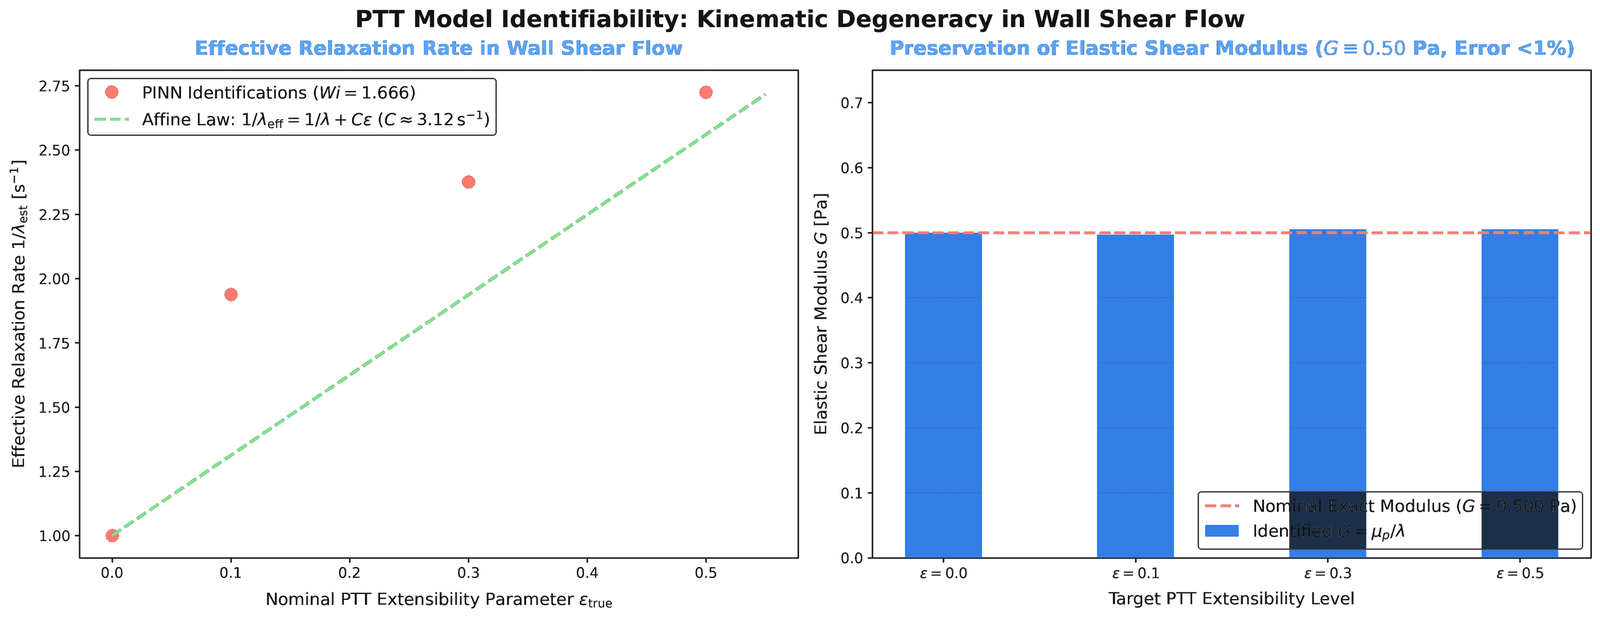
\includegraphics[width=\linewidth]{media/fig6_ptt_degeneracy_insight.png}
    \caption{PTT model identifiability analysis under boundary velocity supervision:
    (left) effective relaxation rate $1/\lambda_{\mathrm{est}}$ as a function of
    nominal extensibility $\varepsilon_{\mathrm{true}}$ in wall shear flow, compared
    with the affine shift law ($C \approx 3.12\,\mathrm{s}^{-1}$);
    (right) preservation of the composite elastic shear modulus
    $G = \mu_p / \lambda = 0.50\,\mathrm{Pa}$ (relative error $< 1.2\%$) across all
    tested PTT extensibility levels, demonstrating macroscopic stiffness conservation
    despite individual parameter degradation.}
    \label{fig:ptt_degeneracy}
\end{figure}

In summary, the computational findings presented throughout this chapter confirm
the predictive capability and delineate the physical identifiability boundaries
of the multi-head PINN framework in viscoelastic flows. In direct mode, the solver
reconstructs unmeasured latent stress and pressure fields with high fidelity
strictly from planar kinematic observations. In inverse mode, the network reliably
discovers nonlinear constitutive parameters across linear Oldroyd-B and shear-thinning
Giesekus fluids using only boundary stress anchoring. Simultaneously, the framework
exposes two structural invariance boundaries: the hyperbolic $G$-canyon in mixed
kinematics and the wall-shear degeneracy in linear PTT fluids under boundary velocity
supervision. Chapter~\ref{chap:conclusions} synthesizes these conclusions, discusses
their broader implications for experimental rheometry, and outlines future avenues
for extending physics-informed architectures to three-dimensional and time-dependent
polymeric flows.

    %% !TEX root = ../main.tex
\chapter{Conclusions and Future Perspectives}
\label{chap:conclusions}

This thesis evaluated a Physics-Informed Neural Network (PINN) framework for the
modeling and inverse rheological characterization of steady, two-dimensional
viscoelastic flows in a four-roll mill geometry. By imposing conservation of mass,
momentum balance, and constitutive laws into a decoupled multi-head
architecture, we studied field reconstruction and inverse parameter
estimation. The analysis examined three constitutive models with increasing
nonlinearity: Oldroyd-B, Giesekus, and linear Phan-Thien-Tanner (PTT) fluids.

% ============================================================
% 5.1 SUMMARY OF ACHIEVEMENTS
% ============================================================
\section{Summary of Key Findings and Contributions}
\label{sec:summary_achievements}
\label{sec:conclusions_summary}

The main findings and methodological contributions of this work are organized
along three main aspects:

\begin{enumerate}
    \item \textbf{Decoupled Architecture and Staged Dual-Precision Training}:
    To model the coupled velocity, pressure, and stress fields in a closed
    recirculating cavity, we implemented a three-head neural
    network ($\mathcal{N}_\psi, \mathcal{N}_p, \mathcal{N}_{\boldsymbol{\tau}}$)
    with $\mathrm{SiLU}$ activations and zero initialization for stress and
    pressure. Velocity is parameterized through a scalar stream function
    $\psi(x, y)$, satisfying the divergence-free condition
    ($\nabla \cdot \boldsymbol{u} \equiv 0$) by construction.
    Pressure gauge indeterminacy is resolved through an algebraic single-point
    hard anchor.
    Optimization is split into two physical stages: Phase~1 trains kinematics
    and extra-stresses, instead Phase~2 trains momentum balance and pressure
    while keeping the stream function trainable. Combining FP32 Adam for initial
    exploration with FP64 L-BFGS for refinement avoids optimization plateaus and
    yields stable convergence.

    \item \textbf{Direct Latent Field Reconstruction}:
    Supervising planar velocity alone on the canonical Oldroyd-B benchmark
    ($Wi = 0.0833, Re = 0.0417$) enabled the model to reconstruct unmeasured
    viscoelastic stresses and pressure across the domain. Evaluated against a
    finite element reference solution with $125{,}456$ nodes from COMSOL
    Multiphysics, the network achieved relative $L_2$ errors of $0.98\%$ on $u$
    and $0.93\%$ on $v$. Stress prediction errors were $1.21\%$ for shear stress
    $\tau_{xy}$, $1.80\%$ for $\tau_{xx}$, and $1.65\%$ for $\tau_{yy}$, resolving
    the localized stress peaks in the roller gaps. The hydrodynamic pressure field
    was recovered with a range-relative error of $8.13\%$.

    \item \textbf{Inverse Parameter Identification and Transfer Learning}:
    Using planar velocity data and stress supervision on the roller boundaries,
    the inverse PINN identified fluid parameters without interior stress
    measurements. For Oldroyd-B fluids, the relaxation time $\lambda$ and polymeric
    viscosity $\mu_p$ were recovered within $0.41\%$ to $1.27\%$ error across
    both low ($Wi = 0.08$) and moderate ($Wi = 1.17$) elasticity regimes.
    For shear-thinning Giesekus fluids, the network estimated three coupled
    parameters ($\alpha, \lambda, \mu_p$) simultaneously. The mobility factor
    $\alpha$ was identified within $5.76\%$ to $6.70\%$ error, even from distant
    initializations and at the theoretical limit $\alpha = 0.50$.
    Transfer learning halved the required iteration budget from $50{,}000$ to
    $25{,}000$ steps and stabilized optimization at higher Weissenberg numbers.
    Collocation sensitivity tests confirmed that parameter estimates remain stable
    down to $5{,}086$ points.
\end{enumerate}

% ============================================================
% 5.2 OPERATIONAL LIMITATIONS
% ============================================================
\section{Operational Limitations}
\label{sec:limitations}
\label{sec:conclusions_limitations}

Several practical and modeling limitations of the current framework should be
noted:

\begin{itemize}
    \item \textbf{Boundary Stress Anchoring}:
    To break scaling symmetries between polymeric viscosity $\mu_p$ and latent
    stress magnitudes, the inverse solver requires stress supervision on the
    rotating cylinder surfaces ($\mathcal{L}_{\mathrm{roll\_stress}}$).
    Although this avoids domain-wide stress measurements, determining local
    wall shear and normal stresses experimentally requires optical birefringence
    or surface traction sensors.

    \item \textbf{Identifiability of PTT Fluids}:
    When velocity data are concentrated in high-shear regions near the cylinders,
    parameters governing extensional stress saturation, such as the PTT
    extensibility $\varepsilon$, become weakly observable. 

    \item \textbf{Single-Point Pressure Gauge Sensitivity}:
    The algebraic single-point hard anchor is enough from mathematical standpoint
    for the pressure field. However, fixing the gauge at a single peripheral
    node allows local spatial errors in $\nabla p$ to propagate across the domain,
    producing a uniform baseline offset ($18.31\%$ raw relative $L_2$ error
    versus $8.13\%$ after removing the domain mean).

    \item \textbf{Two-Dimensional Steady-State Scope}:
    The present study is restricted to steady, isothermal, two-dimensional flows
    up to moderate Weissenberg numbers ($Wi \le 1.67$). It does not account for
    three-dimensional secondary flows near the roller end-walls, nor does it
    capture time-dependent elastic instabilities that develop at higher
    deformation rates.
\end{itemize}

% ============================================================
% 5.3 FUTURE PERSPECTIVES
% ============================================================
\section{Future Perspectives and Research Directions}
\label{sec:future_outlook}
\label{sec:conclusions_future_work}

The methodology developed in this thesis demonstrates the viability of
decoupled neural solvers for viscoelastic flow fields, while also identifying
several technical extensions:

\begin{enumerate}
    \item \textbf{Changing flow field parameter}:
    The present benchmark relies on four identical counter-rotating cylinders,
    which enforce purely extensional flow at the cavity center. Future work
    should evaluate asymmetric or time-dependent boundary kinematics, such as
    independent cylinder rotation speeds or alternating drive ratios. Testing
    these configurations will verify whether the decoupled architecture adapts
    to mixed shearing and extensional dynamics.

    \item \textbf{Addition of Gaussian Noise}:
    The synthetic datasets used throughout this work represent ideal, noise-free
    velocity fields. Adding controlled Gaussian noise to planar
    velocity and roller boundary observations will establish the sensitivity of
    automatic differentiation under realistic experimental conditions. This step
    will define the signal-to-noise threshold below which the loss formulation
    requires explicit smoothing filters orr egularization.

    \item \textbf{Exponential Constitutive PTT}:
    The current study implemented linear PTT fluids, in which the stress trace
    enters linearly as $1 + (\varepsilon \lambda / \mu_p)\mathrm{tr}(\boldsymbol{\tau})$.
    Extending the formulation to the exponential PTT (ePTT) model, where
    $Y(\mathrm{tr}(\boldsymbol{\tau})) = \exp[(\varepsilon \lambda / \mu_p)\mathrm{tr}(\boldsymbol{\tau})]$,
    introduces steeper nonlinear gradients during backpropagation. Investigating
    ePTT will test whether the staged optimization scheme remains stable when
    confronted with exponential stress growth near stagnation lines.

    \item \textbf{Convergence Mapping Across Parameter Space}:
    Systematic parameter sweeps across Weissenberg numbers ($Wi$), Reynolds numbers
    ($Re$), and loss weightings are needed to map the convergence boundaries of
    the solver. This research will identify the precise
    threshold where this framework is still appliable. 
\end{enumerate}

\vspace{0.5em}
Overall, physics-informed neural networks offer a flexible alternative to purely
empirical data fitting and traditional mesh-based discretizations in rheological
characterization. By embedding continuum momentum balance and constitutive laws
directly into the objective function,our work reconstructs unmeasured
stress fields and identifies nonlinear material parameters from sparse kinematic
data. The decoupled formulation and staged training sequence resolve the
numerical stiffness typically associated with coupled viscoelastic equations,
providing a foundation for hybrid experimental-computational rheometry.


    %\chapter*{Appendice}
    \bibliographystyle{unsrt}
    \bibliography{references}
\end{document}
